\documentclass[12pt,a4paper]{article}
\usepackage[utf8]{inputenc}[spanish]
\usepackage{amsmath}
\usepackage{amsfonts}
\usepackage{amssymb}
\usepackage{lmodern}
\usepackage{amsmath}
\usepackage{amsthm}
\usepackage{enumerate}
\usepackage{graphicx}
\usepackage{mathtools}
\usepackage{stackrel}
\usepackage{multicol}
\usepackage{amsmath}
\usepackage{amsfonts}
\usepackage{amssymb}
\usepackage{lmodern}
\usepackage{amsmath}
\usepackage{enumerate}
\usepackage{algorithmic}
\usepackage{algorithm}
\usepackage{graphicx}
\usepackage{mathtools}
\usepackage{gensymb}
\usepackage[left=2cm,right=2cm,top=2cm,bottom=2cm]{geometry}
\newcommand{\PN}{\par\noindent}
\newcommand{\VS}{\vspace{3mm}}
\providecommand{\abs}[1]{\lvert#1\rvert}

\author{Agustín Curto, agucurto95@gmail.com}
\title{Resumen para el final \\ de Física}
\date{2017}

\begin{document}
	\clearpage\maketitle
	\thispagestyle{empty}
	\tableofcontents

	\vspace{5cm}
	\PN \textbf{Nota:} Este resumen se corresponde con la materia dictada en el año 2017. El autor no se responsabiliza de
	posibles cambios que pudiesen realizarse en los temas dictados en la misma, así como tampoco de errores involuntarios
	que pudiesen existir en dicho resumen.

	\vspace{\fill}
	\begin{center}
		Por favor, mejorá este documento en github
		
\includegraphics[width=1cm]{graphics/github.png} \\
		https://github.com/ResumenesFaMAF/resumenFisica
	\end{center}

	\pagebreak
	
	\part{Mecánica}
		\section{Física y medición}
  \subsection{Estándares de longitud, masa y tiempo}
    \PN En mecánica, las tres cantidades fundamentales son longitud, masa y tiempo. Todas las otras cantidades en
    mecánica se pueden expresar en función de estas tres.

    \PN En 1960, un comité internacional estableció un conjunto de estándares para las cantidades fundamentales de la
    ciencia. Se llama \textbf{Sistema Internacional} (SI)) y sus unidades fundamentales de \textbf{longitud},
    \textbf{masa} y \textbf{tiempo} son metro, kilogramo y segundo, respectivamente. Otros estándares para las unidades
    fundamentales SI establecidas por el comité son las de temperatura (el \textit{kelvin}), corriente eléctrica (el
    \textit{ampere}), etc.
    \begin{itemize}
      \item Longitud: La distancia entre dos puntos en el espacio se identifica como \textbf{longitud}. El
      \textbf{metro} se redefinió como la distancia recorrida por la luz en el vacío durante un tiempo de 1/299 792 458
      segundos.
      \item Masa: La unidad fundamental de masa en el SI, el \textbf{kilogramo} (kg), está definida como la masa de un
      cilindro de aleación platino–iridio específico.
      \item Tiempo: La unidad fundamental es el \textbf{segundo} que se define como 9 192 631 770 veces el periodo de
      vibración de la radiación del átomo de cesio 133.
    \end{itemize}

		\section{Movimiento en una dimensión}
  \subsection{Posición, velocidad y repidez}
    \begin{itemize}
      \item La \textbf{posición} x de una partícula es la ubicación de la partícula respecto a un punto de referencia
      elegido que se considera el origen de un sistema coordenado. El movimiento de una partícula se conoce por completo
      si la posición de la partícula en el espacio se conoce en todo momento.

      \item El \textbf{desplazamiento} $\Delta x$ de una partícula se define como su cambio en posición en algún
      intervalo de tiempo. Conforme la partícula se mueve desde una posición inicial $x_{i}$ a una posición final
      $x_{f}$, su desplazamiento está dado por:
      \begin{equation*}
        \Delta x \equiv x_{f} - x_{i}
      \end{equation*}

      \item \textbf{Distancia} es la longitud de una trayectoria seguida por una partícula. La distancia siempre se
      representa como un número positivo, mientras que el desplazamiento puede ser positivo o negativo.
4
      \item La \textbf{velocidad promedio} $v_{x,prom}$ de una partícula se define como el desplazamiento x de la
      partícula dividido entre el intervalo de tiempo $t$ durante el que ocurre dicho desplazamiento:
      \begin{equation*}
        v_{x,prom} \equiv \frac{\Delta x}{\Delta t}
      \end{equation*}

      \item La \textbf{rapidez promedio} $v_{prom}$ de una partícula, una cantidad escalar, se define como la distancia
      total recorrida dividida entre el intervalo de tiempo total requerido para recorrer dicha distancia:
      \begin{equation*}
        v_{prom} \equiv \frac{d}{\Delta t}
      \end{equation*}
    \end{itemize}

  \subsection{Velocidad y rapidez instantáneas}
    \begin{itemize}
      \item La \textbf{velocidad instantánea} $v_{x}$ es igual al valor límite de la razón $\Delta x / \Delta t$
      conforme $\Delta t$ tiende a cero, es decir, a la derivada de x respecto de $t$:
      \begin{equation*}
        v_{x} \equiv \lim_{\Delta t \rightarrow 0} \ \frac{\Delta x}{\Delta t} = \frac{dx}{dt}
      \end{equation*}

      \item La \textbf{rapidez instantánea} de una partícula se define como la magnitud de su velocidad instantánea.
    \end{itemize}

  \subsection{Aceleración}
    \begin{itemize}
      \item La \textbf{aceleración promedio} $a_{x,prom}$ de la partícula se define como el cambio en velocidad $\Delta
      v_{x}$ dividido entre el intervalo de tiempo $t$ durante el que ocurre el cambio:
      \begin{equation*}
        a_{x,prom} \equiv \frac{\Delta v_{x}}{\Delta t} = \frac{v_{xf} - v_{xi}}{t_{f} - t_{i}}
      \end{equation*}

      \item La \textbf{aceleración instantánea} como el límite de la aceleración promedio conforme $\Delta t$ tiende a
      cero.
      \begin{equation*}
        a_{x} \equiv \lim_{\Delta t \rightarrow 0} \ \frac{\Delta v_{x}}{\Delta t} = \frac{dv_{x}}{dt} =
        \frac{d^{2}x}{dt^{2}}
      \end{equation*}
    \end{itemize}

  \subsection{Análisis de modelos}
    \begin{figure}[H]
      \centering
      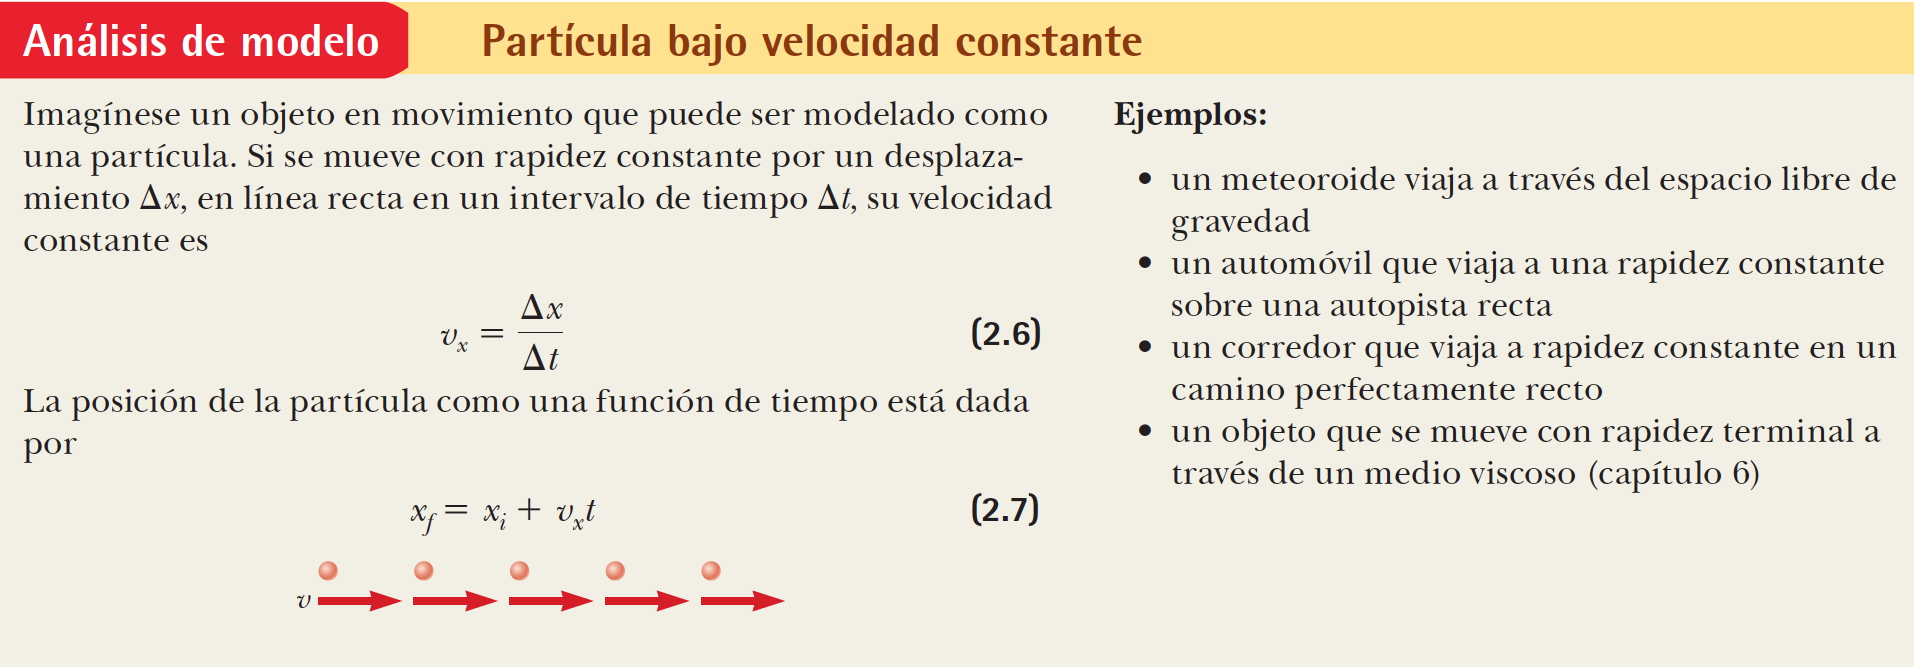
\includegraphics[scale=0.5]{1/graphics_2/figure_0a}
    \end{figure}
    \begin{figure}[H]
      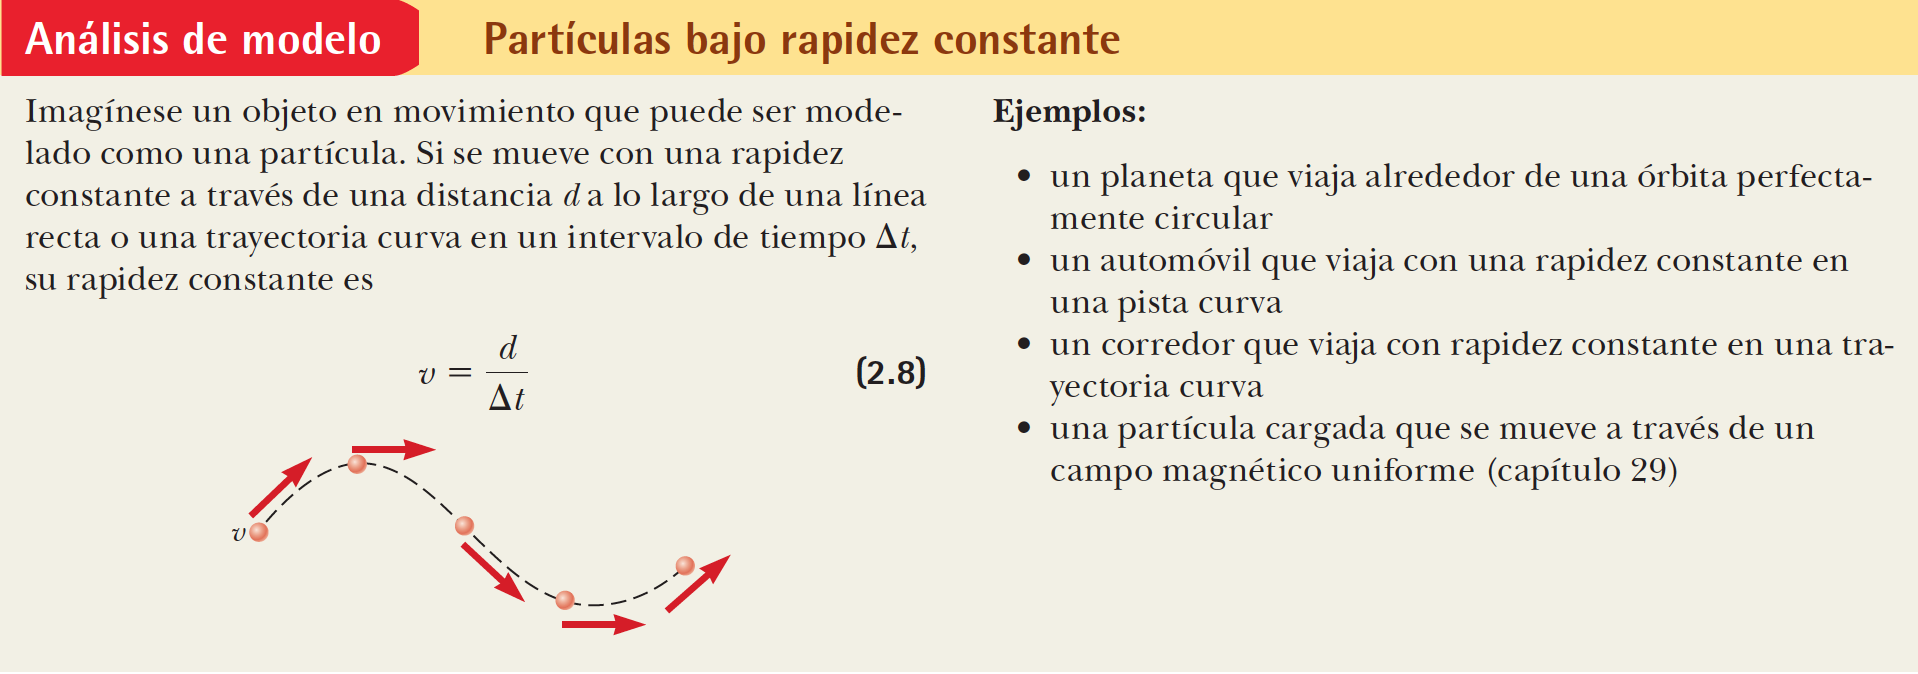
\includegraphics[scale=0.5]{1/graphics_2/figure_0b}
      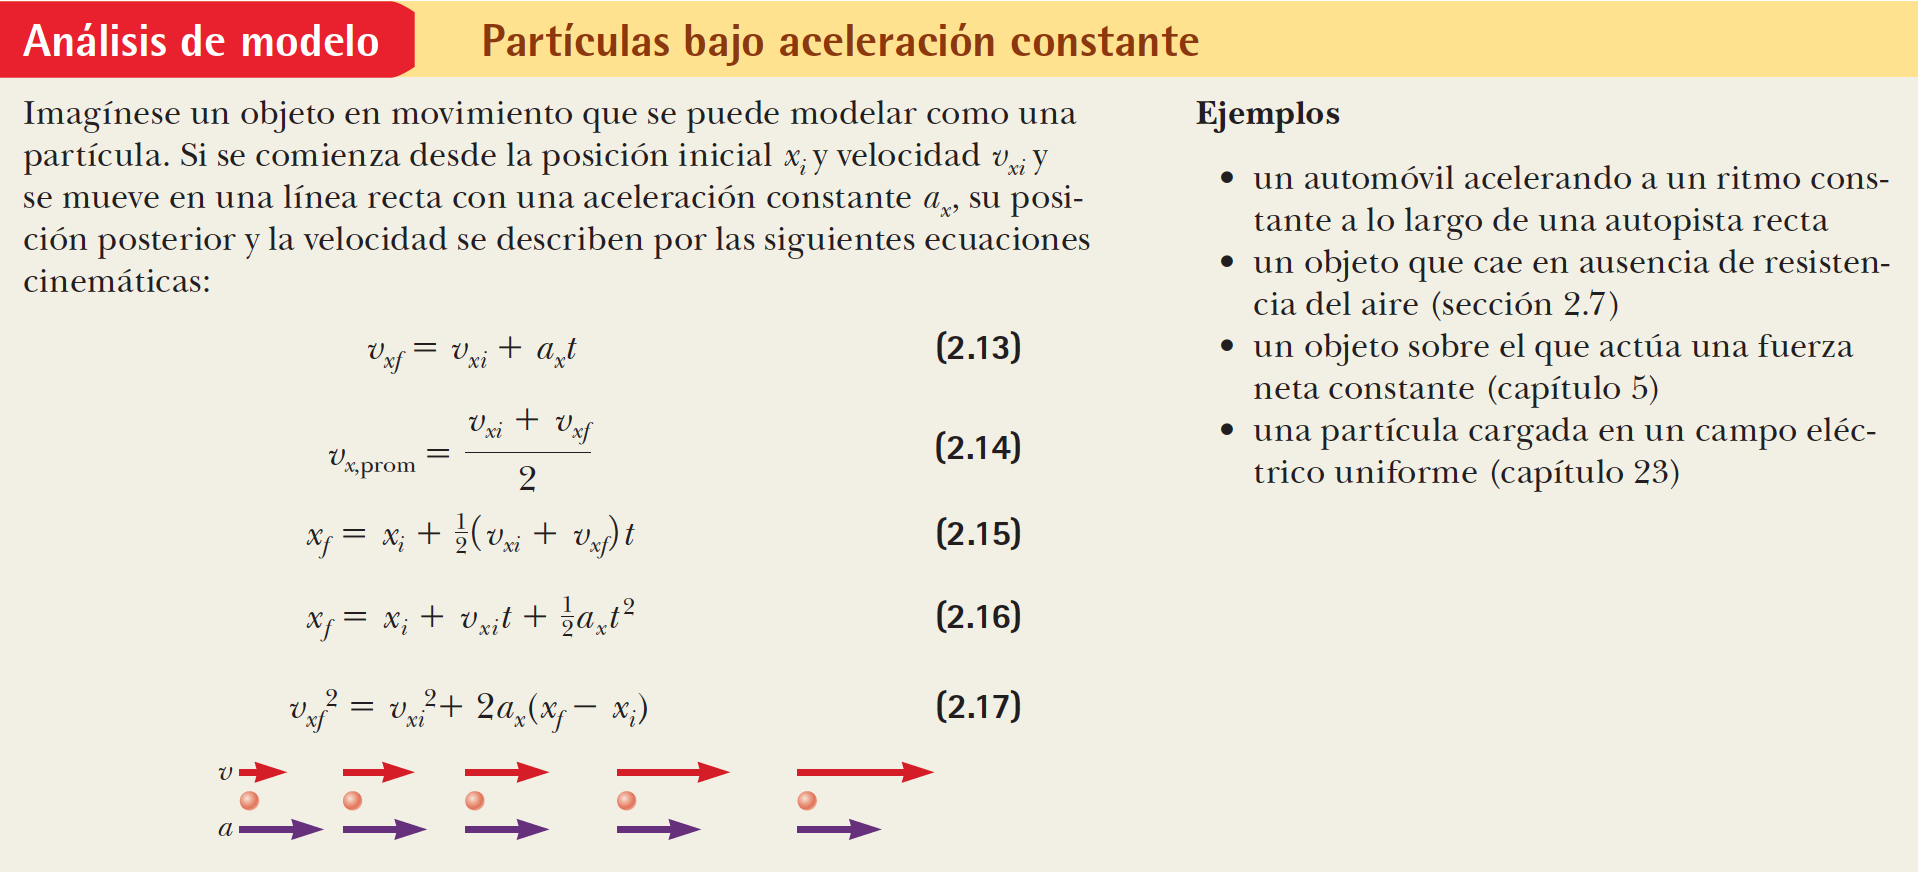
\includegraphics[scale=0.5]{1/graphics_2/figure_0c}
    \end{figure}

  \subsection{Relaciones gráficas entre $x, v_{x}$ y $a_{x}$}
    \begin{figure}[H]
      \centering
      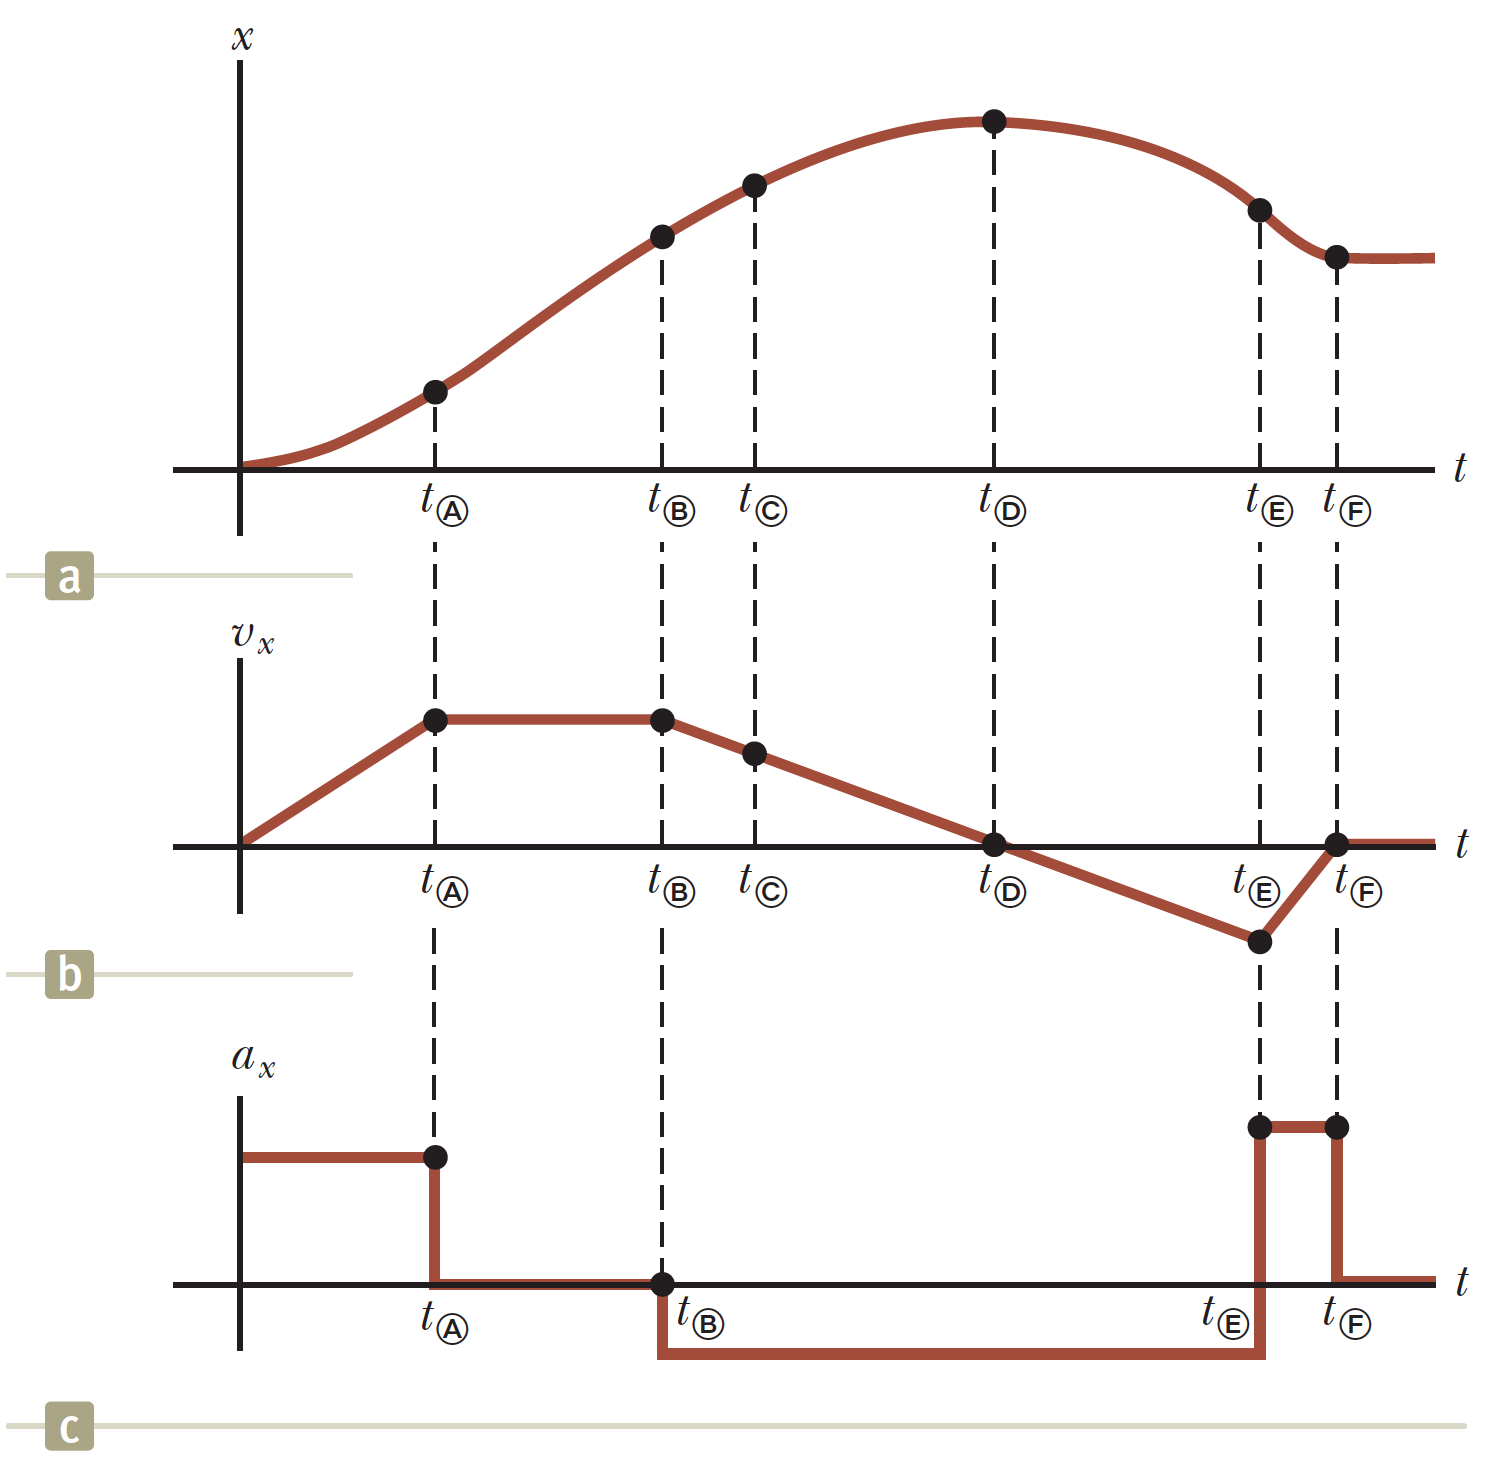
\includegraphics[scale=0.3]{1/graphics_2/figure_1}
      \caption{(a) Gráfica posición-tiempo para un objeto que se mueve a lo largo del eje x. (b) La gráfica
      velocidad-tiempo para el objeto se obtiene al medir la pendiente de la gráfica posición-tiempo en cada instante.
      (c) La gráfica aceleración-tiempo para el objeto se obtiene al medir la pendiente de la gráfica velocidad-tiempo
      en cada instante.}
    \end{figure}

  \subsection{Diagramas de movimiento}
    \PN Con frecuencia los conceptos de \textbf{velocidad} y \textbf{aceleración} se confunden uno con otro, para que
    esto no ocurra, es útil usar una representación pictórica llamada \textit{diagrama de movimiento} para describir la
    velocidad y la aceleración mientras un objeto está en movimiento.

    \begin{figure}[H]
      \centering
      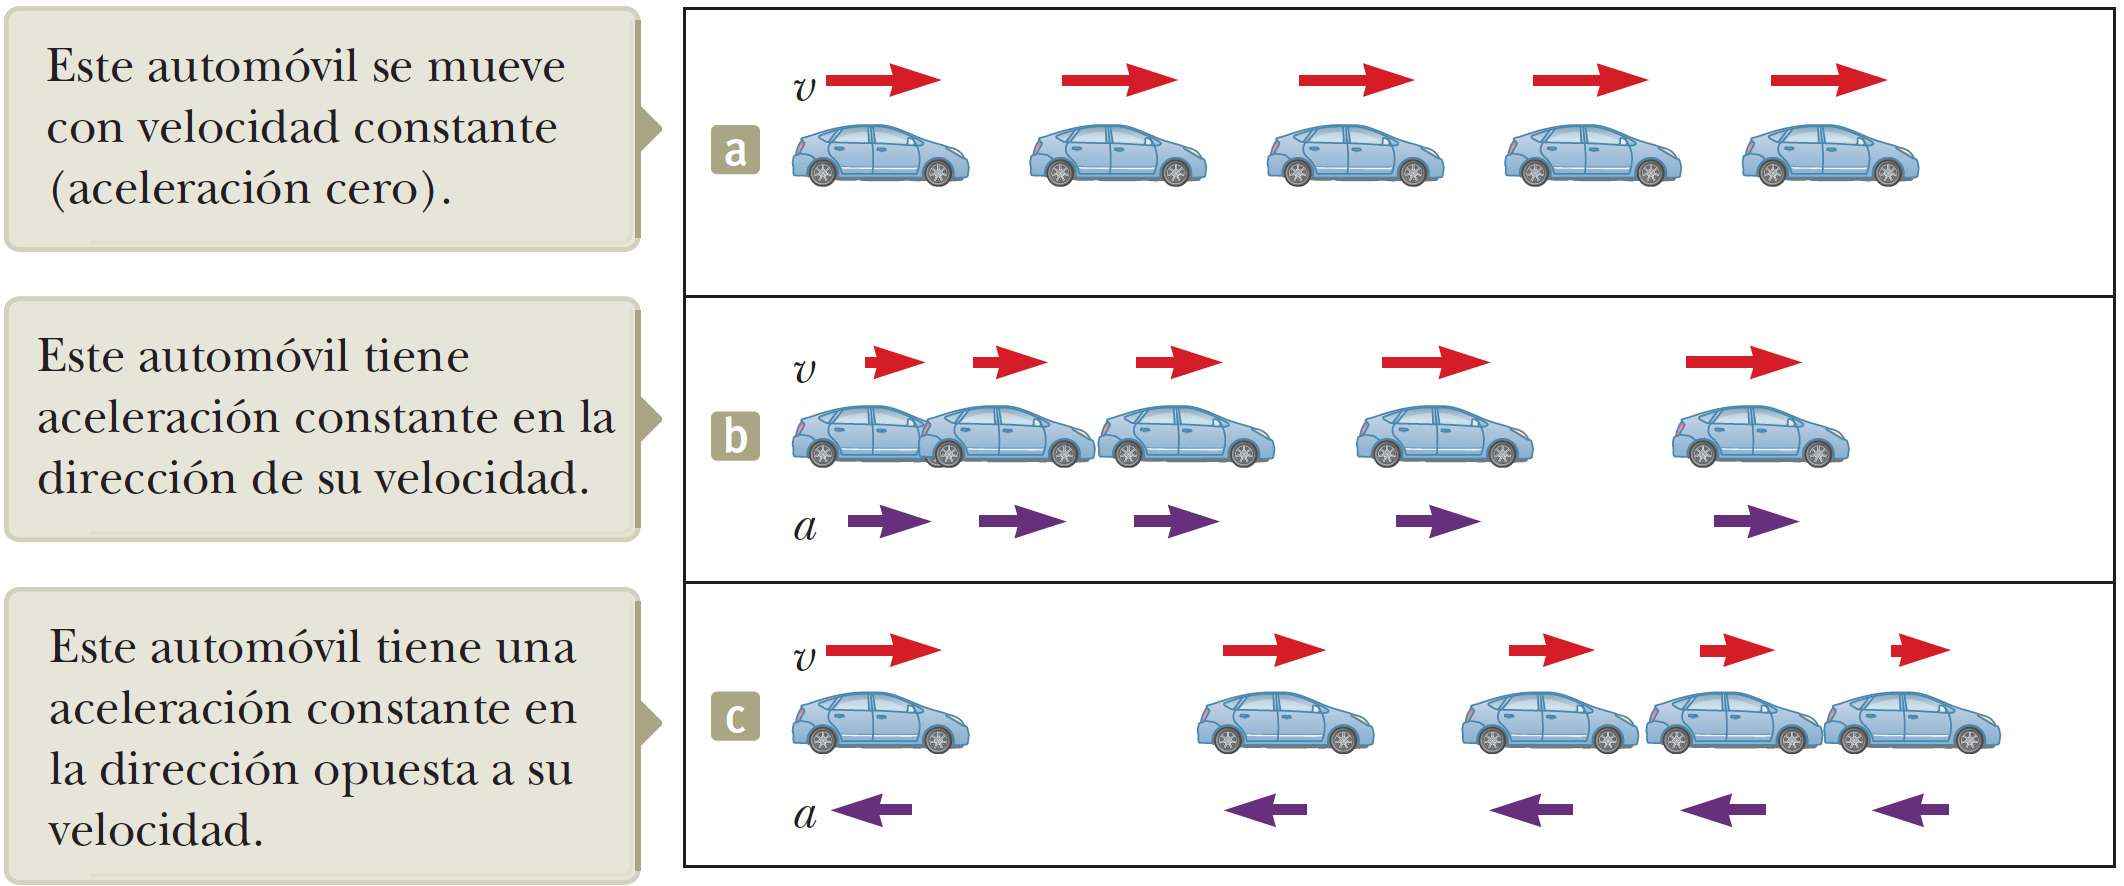
\includegraphics[scale=0.4]{1/graphics_2/figure_2}
      \caption{Diagramas de movimiento de un automóvil que se mueve a lo largo de una carretera recta en una sola
      dirección. La velocidad en cada instante está indicada por una flecha roja, y la aceleración constante se indica
      mediante una flecha de color morado.}
    \end{figure}

  \subsection{Objetos en caída libre}
    \PN En ausencia de resistencia del aire, todos los objetos que se dejan caer cerca de la superficie de la Tierra
    caen hacia ella con la misma aceleración constante bajo la influencia de la gravedad de la Tierra. A dicho
    movimiento se lo conoce como \textit{caída libre}.

    \PN Un objeto en caída libre es cualquier objeto que se mueve libremente sólo bajo la influencia de la gravedad, sin
    importar su movimiento inicial. El movimiento de un objeto en caída libre que se mueve verticalmente es equivalente
    al movimiento de una partícula bajo aceleración constante en una dimensión.

		\section{Vectores}
  \subsection{Sistemas coordenados}
    \PN En el sistema de coordenadas polares $(r, \theta)$, $r$ es la distancia desde el origen hasta el punto que tiene
    coordenadas cartesianas (x, y) y $\theta$ es el ángulo entre un eje fijo y una recta dibujada desde el origen hasta
    el punto. El eje fijo es el eje x positivo y $\theta$ se mide contra el sentido de las agujas del reloj.
    \begin{eqnarray*}
      x = r \ cos(\theta) \\
      y = r \ sen(\theta) \\
      r = \sqrt{x^{2} + y^{2}}
    \end{eqnarray*}

  \subsection{Cantidades vectoriales y escalares}
    \begin{itemize}
      \item Una \textbf{cantidad escalar} se especifica por completo mediante un valor único con una unidad adecuada y
      no tiene dirección.
      \item Una \textbf{cantidad vectorial} se especifica por completo mediante un número y unidades apropiadas más una
      dirección.
    \end{itemize}

		\section{Movimiento en dos dimensiones}

		\section{Las leyes del movimiento}
  \subsection{Concepto de fuerza}
    \PN Clasificación de un fuerza según contacto:
    \begin{itemize}
      \item \textbf{Fuerza de contacto:} implican contacto físico entre dos objetos.
        \begin{figure}[H]
          \centering
          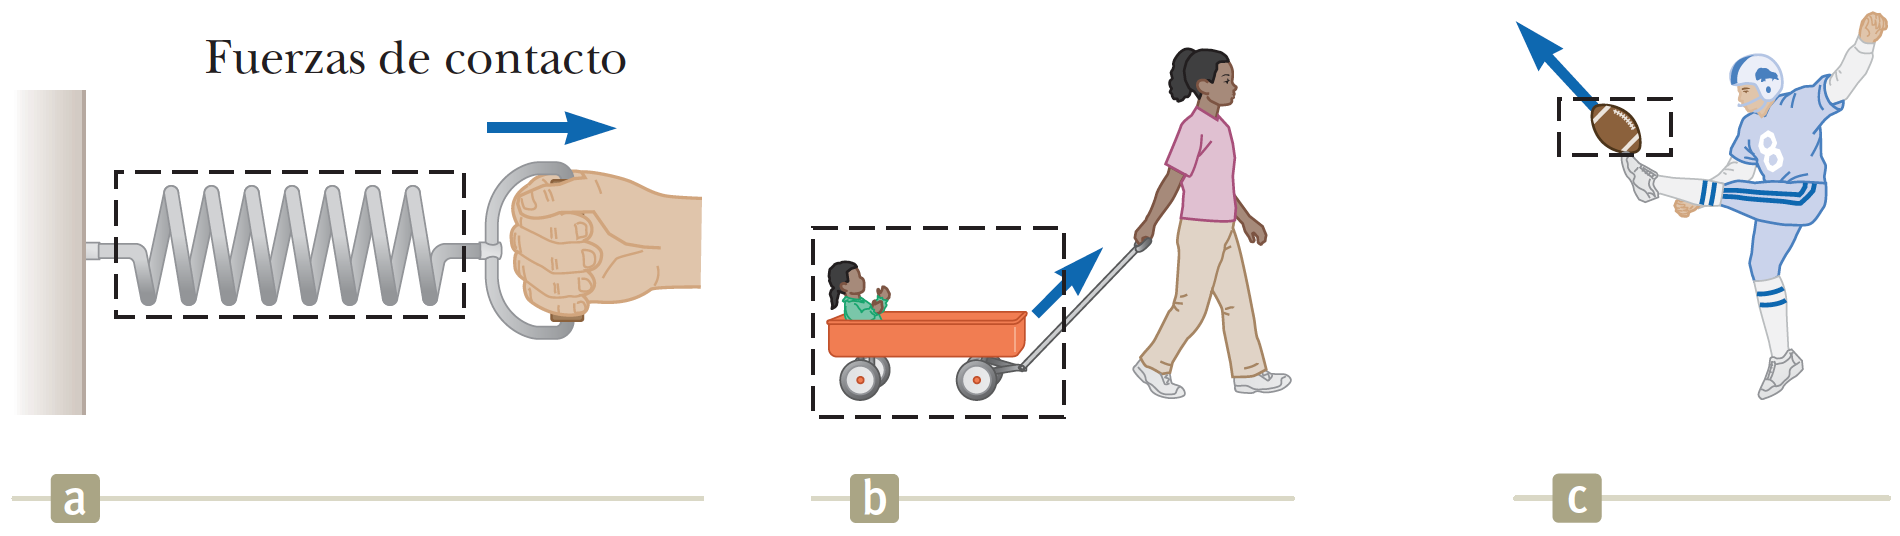
\includegraphics[scale=0.4]{1/graphics_5/figure_0}
          \caption{Una partícula que se mueve en el plano xy se ubica con el vector de posición $\BV{r}$, que se dibuja
          desde el origen hasta la partícula.}
        \end{figure}

      \item \textbf{Fuerza de campo:} no involucran contacto físico entre dos objetos.
        \begin{figure}[H]
          \centering
          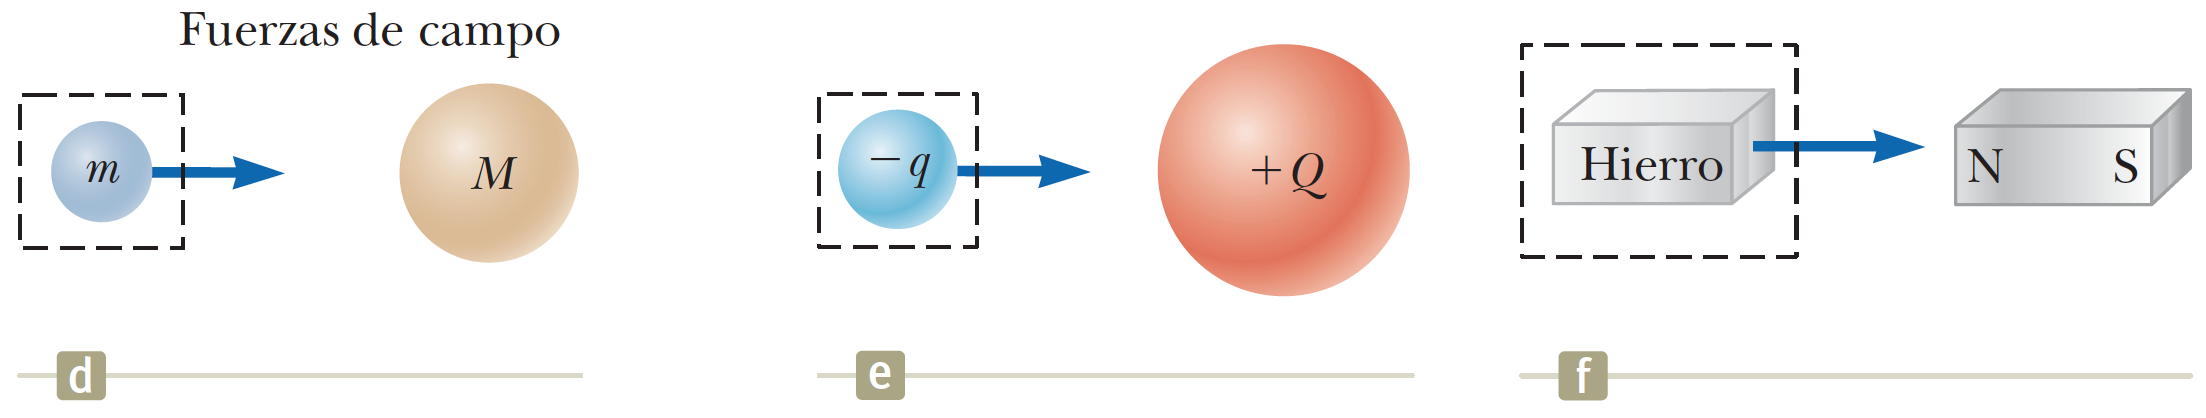
\includegraphics[scale=0.4]{1/graphics_5/figure_1}
          \caption{Una partícula que se mueve en el plano xy se ubica con el vector de posición $\BV{r}$, que se dibuja
          desde el origen hasta la partícula.}
        \end{figure}
    \end{itemize}

    \PN La distinción entre \textit{fuerzas de contacto} y \textit{fuerzas de campo} no es tan clara como se podría
    pensar. Cuando se examinan a nivel atómico, todas las fuerzas que se clasifican como fuerzas de contacto resultan
    ser causadas por fuerzas (de campo) eléctricas. Las únicas \textbf{fuerzas fundamentales} conocidas en la naturaleza
    son todas fuerzas de campo:
    \begin{enumerate}
      \item fuerzas gravitacionales entre objetos
      \item fuerzas electromagnéticas entre cargas eléctricas
      \item fuerzas fuertes entre partículas subatómicas
      \item fuerzas débiles que surgen en ciertos procesos de decaimiento radiactivo
    \end{enumerate}

    \PN En la física clásica sólo interesan las fuerzas gravitacional y electromagnética.

  \subsection{Primera ley de Newton y marcos inerciales}
    \PN La primera ley del movimiento de Newton, a veces llamada \textit{ley de la inercia}, define un conjunto especial
    de marcos de referencia llamados marcos inerciales. Esta ley se puede establecer del modo siguiente:

    \begin{tcolorbox}
      Si un objeto no interactúa con otros objetos, es posible identificar un marco de referencia inercial en el que el
      objeto tiene aceleración cero.
    \end{tcolorbox}

    \PN Tal marco de referencia se llama \textbf{marco de referencia inercial}.

    \PN Se puede plantear un enunciado más práctico de la primera ley del movimiento de Newton:

    \begin{tcolorbox}
      En ausencia de fuerzas externas, y cuando se ve desde un marco de referencia inercial, un objeto en reposo se
      mantiene en reposo y un objeto en movimiento continúa en movimiento con una velocidad constante (esto es, con una
      rapidez constante en una línea recta).
    \end{tcolorbox}

    \PN En otras palabras, cuando ninguna fuerza actúa sobre un objeto, la aceleración del objeto es cero. La tendencia
    de un objeto a resistir cualquier intento por cambiar su velocidad se llama inercia. Se puede concluir que un objeto
    que acelera debe experimentar una fuerza. A su vez, de la primera ley, se puede definir fuerza como aquello que
    causa un cambio en el movimiento de un objeto.

  \subsection{Masa}
    \PN La masa es la propiedad de un objeto que especifica cuánta resistencia muestra un objeto para cambiar su
    velocidad. Los experimentos muestran que mientras más grande sea la masa de un objeto, menos acelera el objeto bajo
    la acción de una fuerza aplicada conocida.

    \PN Suponga que una fuerza que actúa sobre un objeto de masa $m_{1}$ produce un cambio en el movimiento de éste que
    puede cuantificarse mediante la aceleración $\BV{a}_{1}$ del objeto, y la misma fuerza sobre un cuerpo de masa
    $m_{2}$ produce una aceleración $\BV{a}_{2}$. La razón de las dos masas se define como la razón inversa de las
    magnitudes de las aceleraciones producidas por la fuerza:

    \[
      \frac{m_{1}}{m_{2}} \equiv \frac{a_{2}}{a_{1}}
    \]

    \PN La magnitud de la aceleración de un objeto es inversamente proporcional a su masa cuando sobre él actúa una
    fuerza conocida.

    \PN La masa no se debe confundir con el peso. La masa y el peso son dos cantidades diferentes. El peso de un objeto
    es igual a la magnitud de la fuerza gravitacional ejercida sobre el objeto y varía con la posición.

  \subsection{Segunda ley de Newton}
    \PN La segunda ley de Newton responde la pregunta de qué le ocurre a un objeto que tiene una o más fuerzas que
    actúan sobre él. La aceleración de un objeto es directamente proporcional a la fuerza que actúa sobre él:
    $\BV{F} \propto \BV{a}$. La magnitud de la aceleración de un objeto es inversamente proporcional a su masa,
    $\abs{\BV{a}} \propto \frac{1}{m}$.

    \PN Estas observaciones experimentales se resumen en la segunda ley de Newton:

    \begin{tcolorbox}
      Cuando se ve desde un marco de referencia inercial, la aceleración de un objeto es directamente proporcional a la
      fuerza neta que actúa sobre él e inversamente proporcional a su masa:

      \[
        \BV{a} \propto \frac{\sum \BV{F}}{m}
      \]
    \end{tcolorbox}

    \PN Si se elige una constante de proporcionalidad 1, se relaciona masa, aceleración y fuerza a través del siguiente
    enunciado matemático de la segunda ley de Newton:

    \[
      \sum \BV{F} = m \BV{a}
    \]

    \PN La fuerza neta sobre un objeto es la suma vectorial de todas las fuerzas que actúan sobre el objeto. A veces a
    la fuerza neta se le referirá como fuerza total, fuerza resultante o fuerza desbalanceada.

  \subsection{Fuerza gravitacional y peso}
    \PN La fuerza de atracción que ejerce la Tierra sobre un objeto se llama \textbf{fuerza gravitacional} $\BV{f}_{g}$.
    Esta fuerza se dirige hacia el centro de la Tierra y su magnitud se llama peso del objeto. Al aplicar la segunda ley
    de Newton $\sum \BV{F} = m \BV{a}$ a un objeto en caída libre de masa $m$, con $\BV{a} = \BV{g}$ y
    $\sum \BV{F} = \BV{F}_{g}$ se obtiene:

    \[
      \BV{F}_{g} = m \BV{g}
    \]

    \PN Por lo tanto, el peso de un objeto, al definirse como la magnitud de $\BV{F}_{g}$, está dado por:

    \[
      F_{g} = m g
    \]

    \PN Esta ecuación cuantifica la fuerza gravitacional sobre el objeto, pero note que no requiere que el objeto se
    mueva. Incluso para un objeto fijo o para un objeto sobre el que actúan varias fuerzas, la ecuación se puede aplicar
    para calcular la magnitud de la fuerza gravitacional. La masa $m$ en la ecuación anterior establece la intensidad de
    la atracción gravitacional entre el objeto y la Tierra. Este papel es por completo diferente del descrito antes para
    la masa: medir la resistencia al cambio en movimiento como respuesta a una fuerza externa. En ese papel, la masa
    también es llamada \textbf{masa inercial}. Por ende, la $m$ en la ecuación anterior se llama
    \textbf{masa gravitacional}.

  \subsection{Tercera ley de Newton}
    \PN Las fuerzas son \textit{interacciones} entre dos objetos, este importante principio se conoce como
    \textbf{tercera ley de Newton}.

    \begin{tcolorbox}
      Si dos objetos interactúan, la fuerza $\BV{F}_{12}$ que ejerce el objeto 1 sobre el objeto 2 es igual en magnitud
      y opuesta en dirección a la fuerza $\BV{F}_{21}$ que ejerce el objeto 2 sobre el objeto 1:

      \[
        \BV{F}_{12} = - \BV{F}_{21}
      \]
    \end{tcolorbox}

    \PN Cuando sea importante designar fuerzas como interacciones entre dos objetos, se usará esta notación de
    subíndices, donde $\BV{F}_{ab}$ significa \textquotedblleft la fuerza ejercida por a sobre b\textquotedblright.

    \vspace{3mm}
    \PN La tercera ley se ilustra en la siguiente figura. La fuerza que el objeto 1 ejerce sobre el objeto 2 se llama
    popularmente \textit{fuerza de acción}, y la fuerza del objeto 2 sobre el objeto 1 se llama
    \textit{fuerza de reacción}.

    \begin{figure}[H]
      \centering
      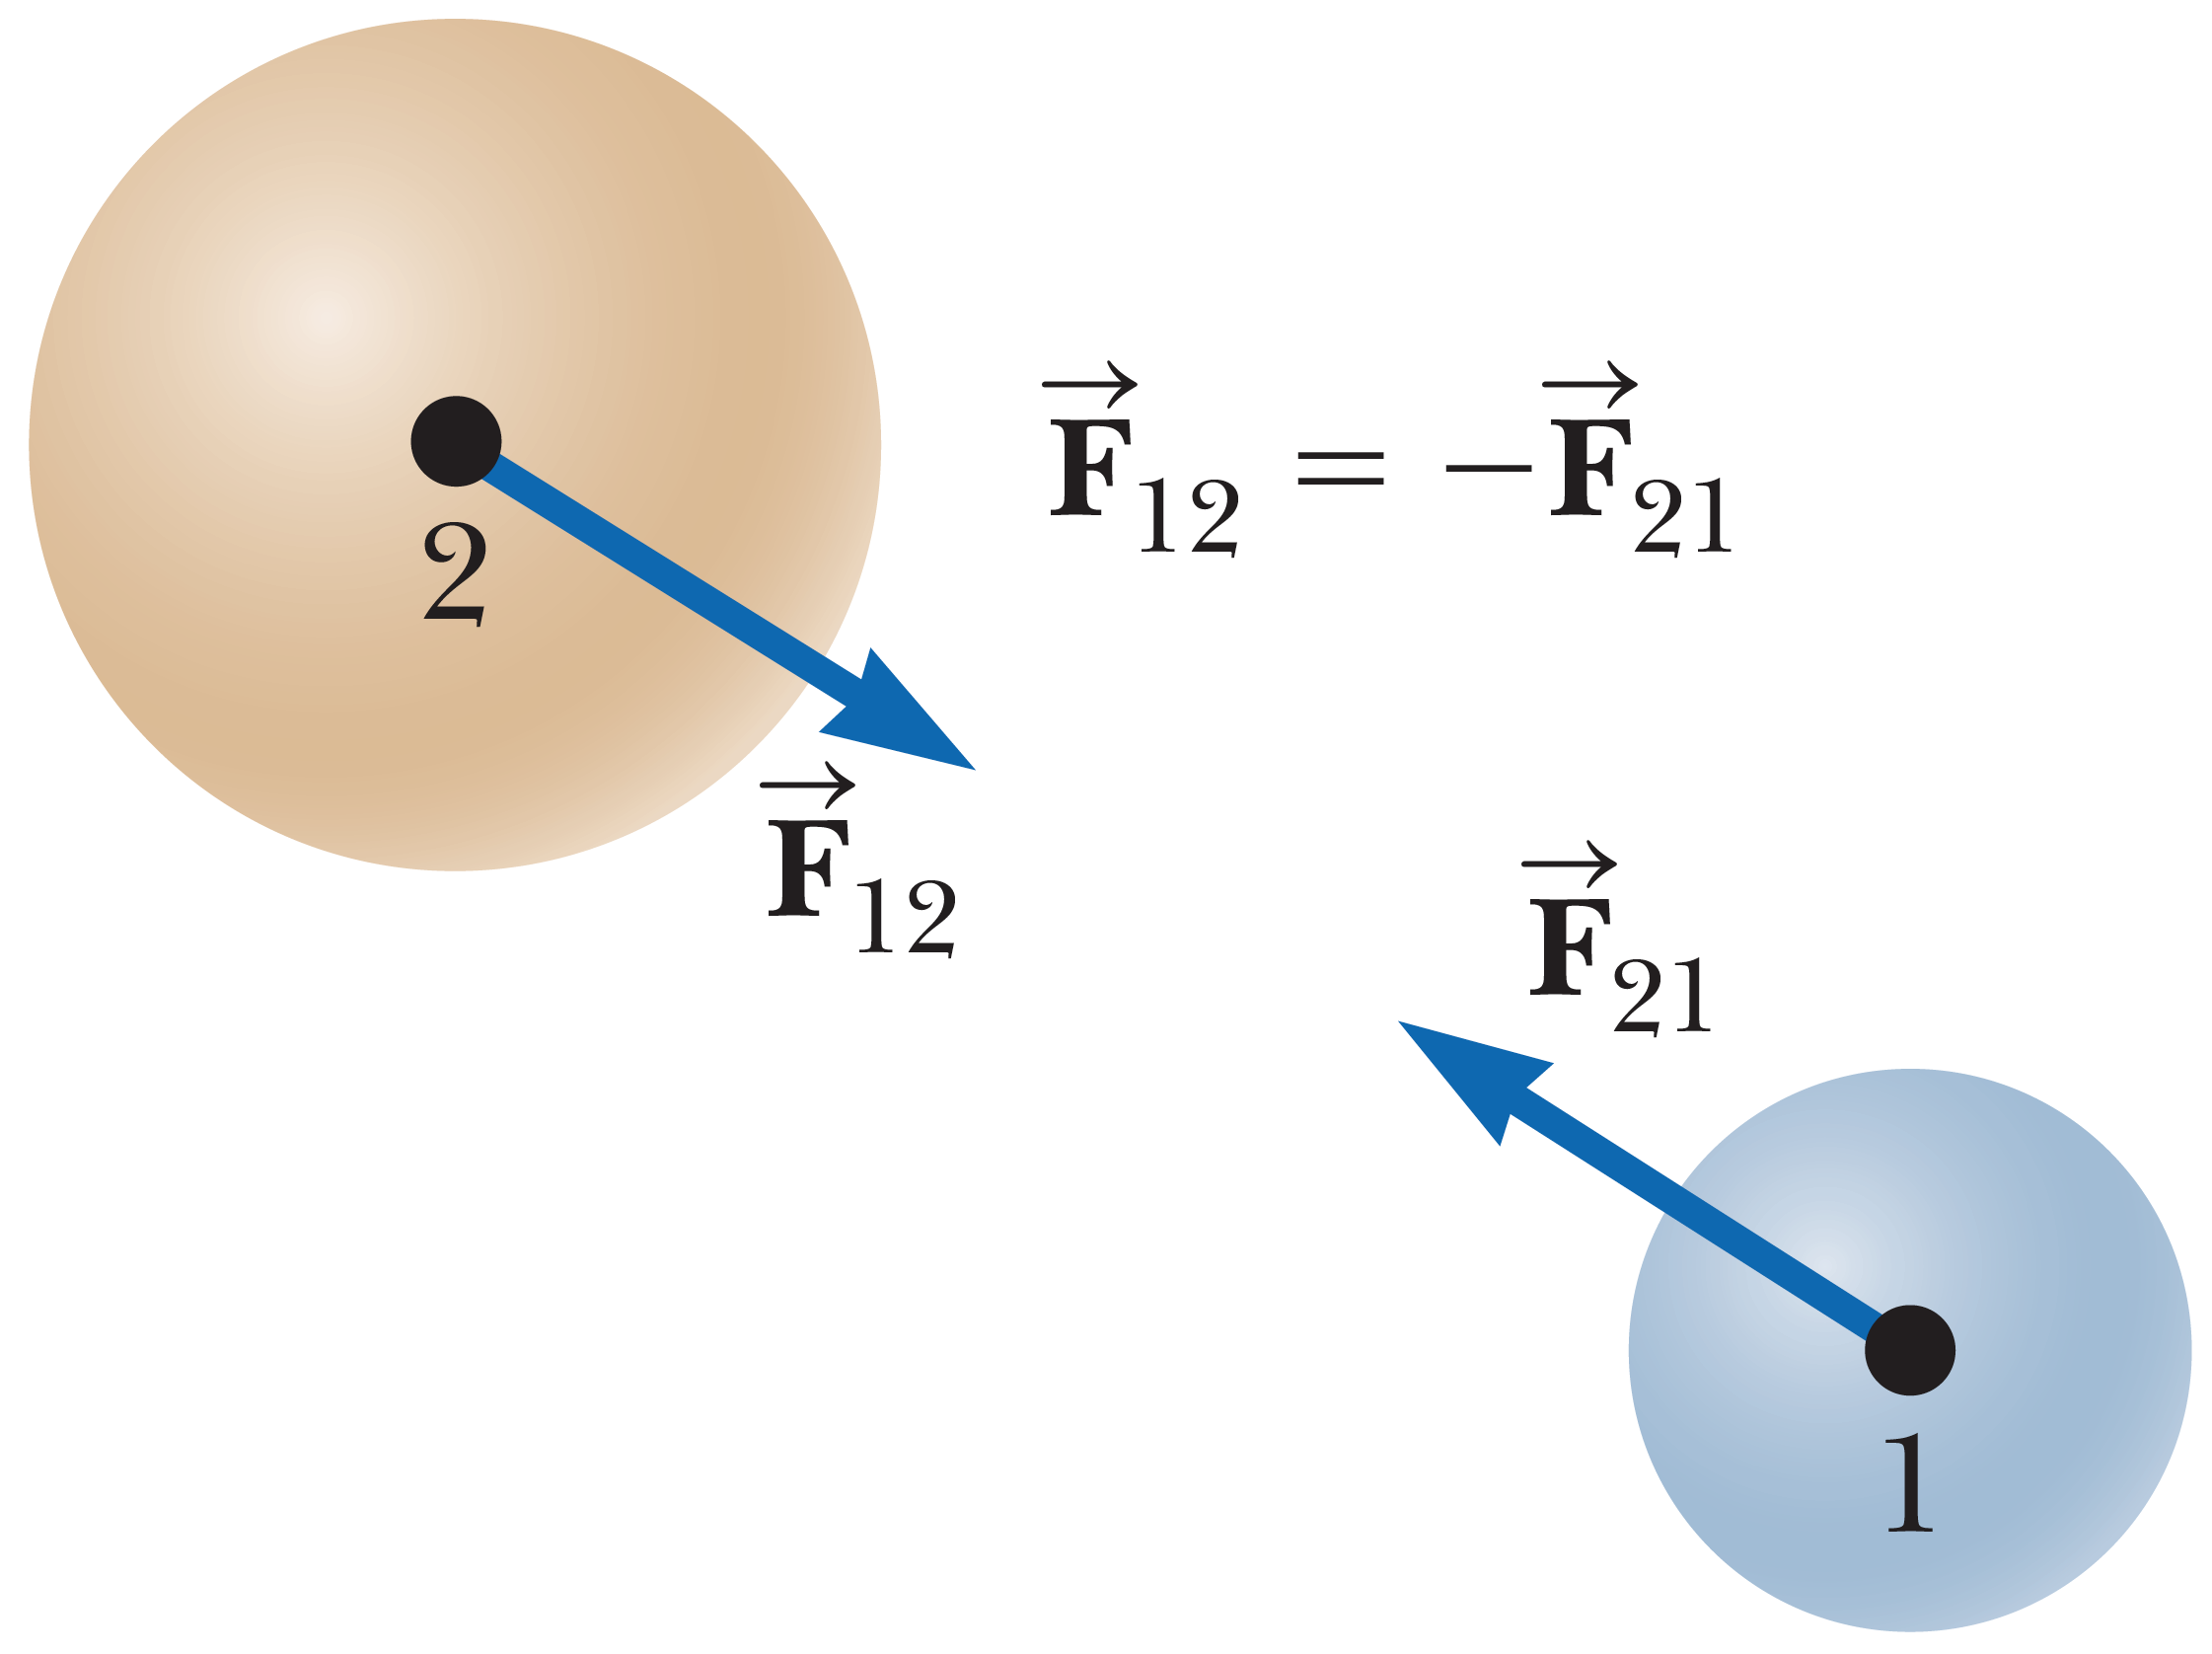
\includegraphics[scale=0.15]{1/graphics_5/figure_2}
      \caption{Tercera ley de Newton. La fuerza $\BV{F}_{12}$ que ejerce el objeto 1 sobre el objeto 2 es igual en
      magnitud y opuesta en dirección a la fuerza $\BV{F}_{21}$ que ejerce el objeto 2 sobre el objeto 1.}
    \end{figure}

    \PN Considere un monitor de computadora en reposo sobre una mesa, como en la figura siguiente. El monitor no acelera
    porque lo sostiene la mesa (t). La mesa ejerce sobre el monitor una fuerza hacia arriba $\BV{n} = \BV{F}_{tm}$,
    llamada \textbf{fuerza normal}. En general, siempre que un objeto esté en contacto con una superficie, ésta ejerce
    una fuerza normal sobre el objeto. Puesto que el monitor tiene aceleración cero, la segunda ley de Newton aplicada
    al monitor produce $\sum \BV{F} = \BV{n} + m \BV{g} = 0$, de modo que $n = mg$. La fuerza normal equilibra la fuerza
    gravitacional sobre el monitor, de modo que la fuerza neta sobre el monitor es cero.

    \begin{figure}[H]
      \centering
      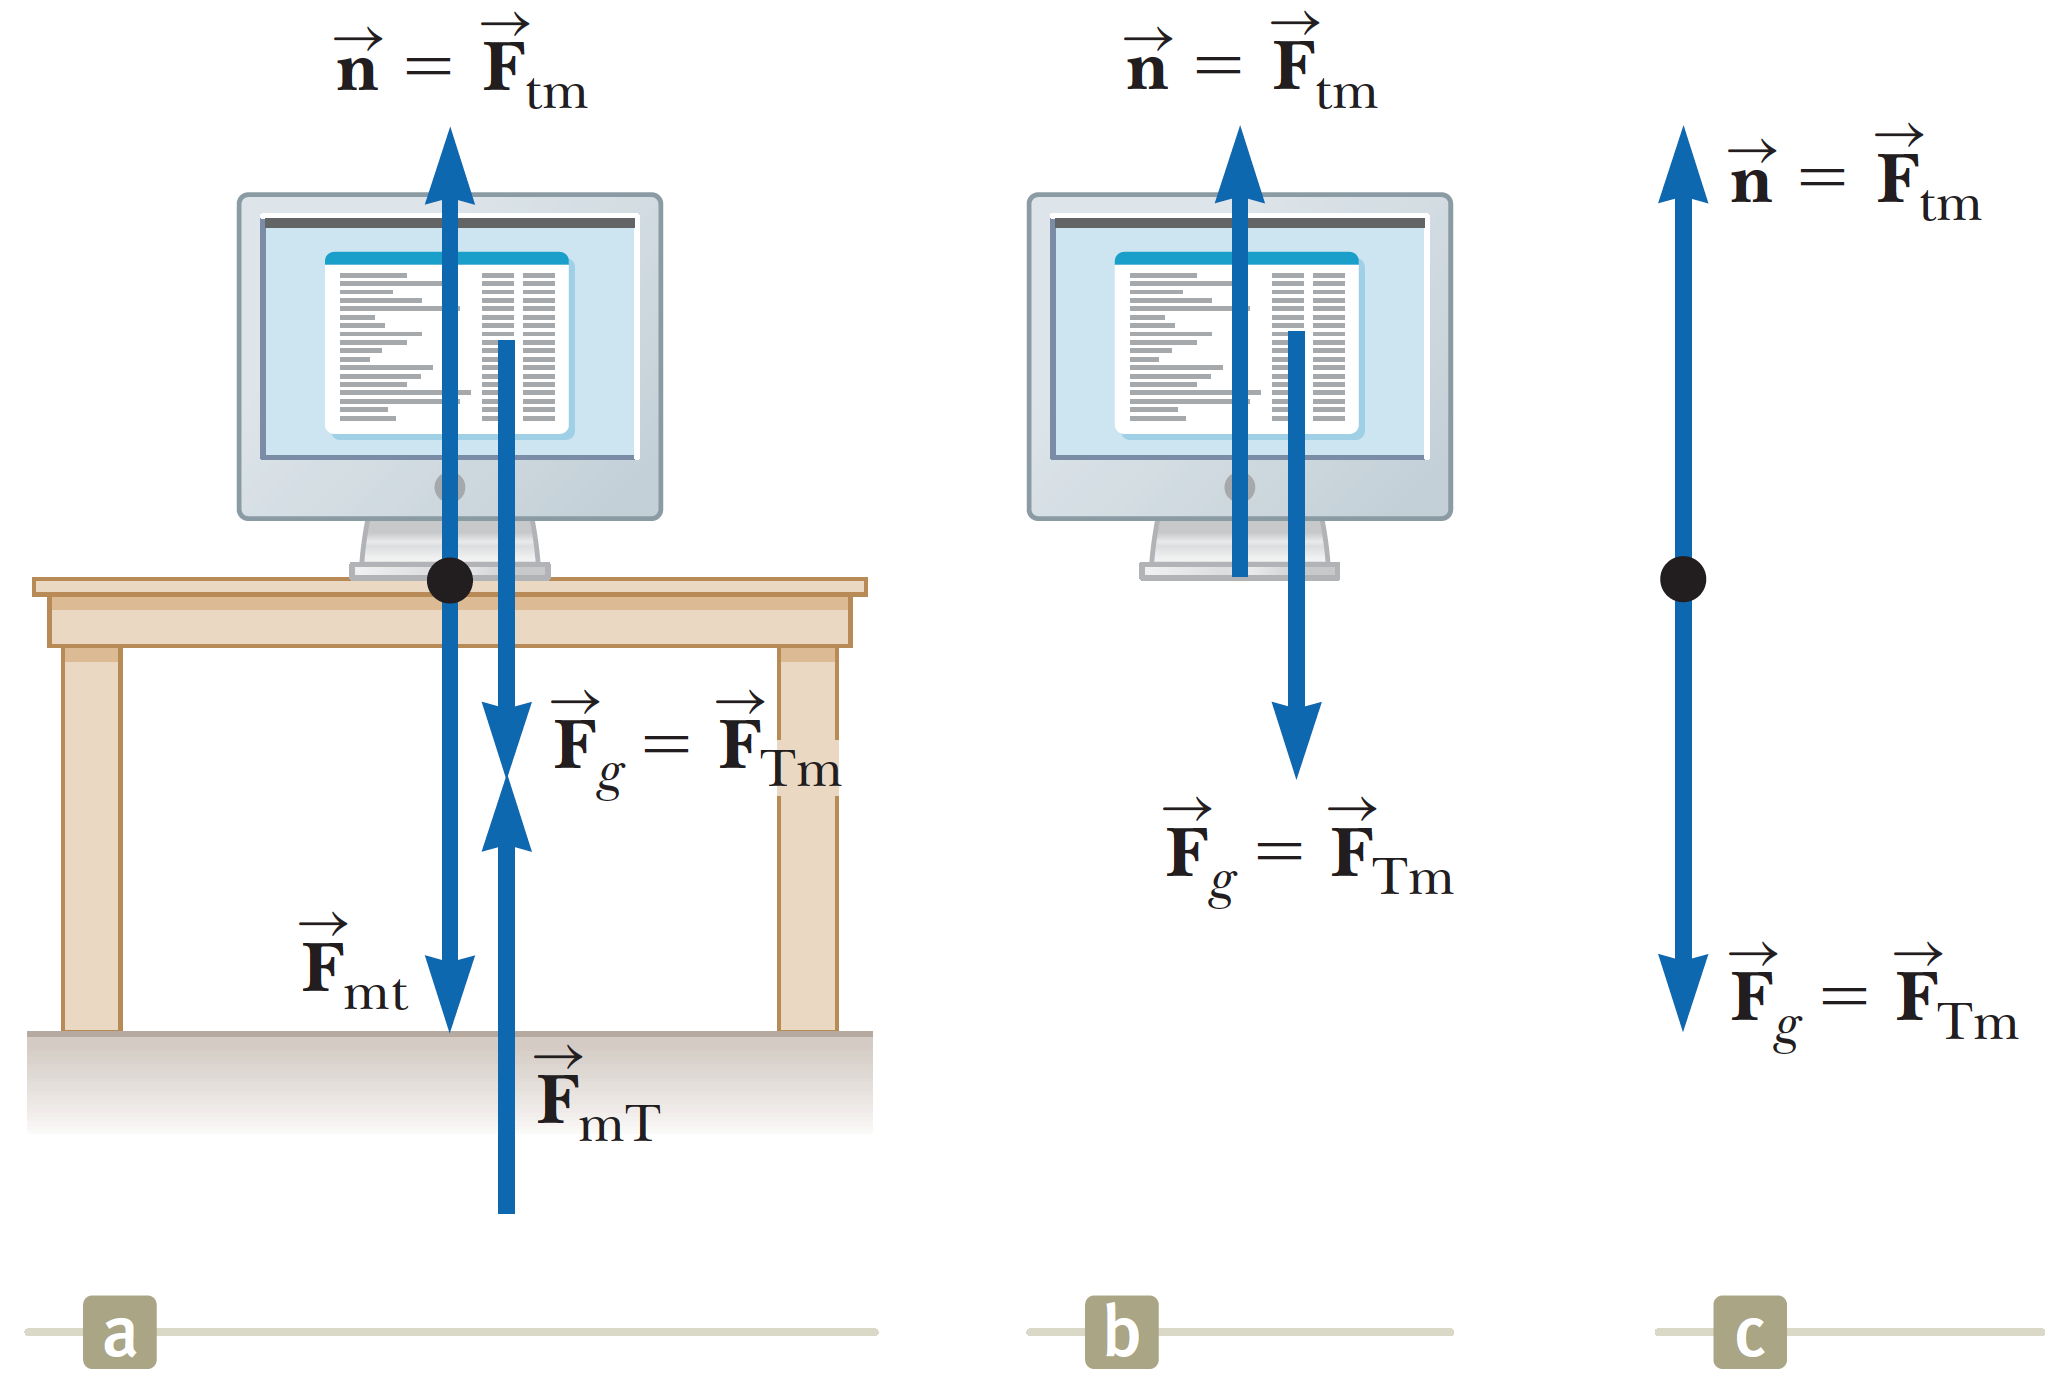
\includegraphics[scale=0.3]{1/graphics_5/figure_3}
      \caption{(a) Cuando un monitor de computadora está en reposo sobre una mesa, las fuerzas que actúan sobre el
      monitor son la fuerza normal $\BV{n}$ y la fuerza gravitacional $\BV{F}_{g}$. La reacción a $\BV{n}$ es la fuerza
      $\BV{F}_{mt}$ que ejerce el monitor sobre la mesa. La reacción a $\BV{F}_{g}$ es la fuerza $\BV{F}_{mT}$ que
      ejerce el monitor sobre la Tierra. (b) Un diagrama de fuerzas muestra las fuerzas sobre el monitor. (c) Un
      diagrama de cuerpo libre mostrando al monitor como un punto negro con las fuerzas actuando sobre él.}
    \end{figure}

  \subsection{Análisis de modelos utilizando la segunda ley de Newton}
    \PN En esta sección se discuten dos análisis de modelos para resolver problemas en que los objetos están en
    equilibrio $(\BV{a} = 0)$ aceleran a lo largo de una línea recta bajo la acción de fuerzas externas constantes. Se
    desprecian los efectos de la fricción en aquellos problemas que involucran movimiento, que es equivalente a afirmar
    que la superficie \textit{no tiene fricción}. Por lo general, se ignora la masa de cualquier soga, cuerda o cable
    involucrado.

    \PN Cuando una cuerda unida a un objeto está jalando al objeto, la cuerda ejerce una fuerza sobre el objeto en una
    dirección que se aleja del objeto, paralela a la cuerda. La magnitud T de dicha fuerza se llama tensión en la cuerda.

    \subsubsection{Análisis de modelo: partícula en equilibrio}
      \PN Si la aceleración de un objeto representado como partícula es cero, el objeto se considera con el modelo de
      \textbf{partícula en equilibrio}. En este modelo, la fuerza neta sobre el objeto es cero:

      \[
        \sum \BV{F} = 0
      \]

    \subsubsection{Análisis de modelo: partícula bajo una fuerza neta}
      \PN Si un objeto experimenta una aceleración, su movimiento se puede analizar con el modelo de partícula bajo una
      fuerza neta. La ecuación apropiada para este modelo es la segunda ley de Newton:

      \[
        \sum \BV{F} = m \BV{a}
      \]

  \subsection{Fuerzas de fricción}
    \PN Cuando un objeto está en movimiento, ya sea sobre una superficie o en un medio viscoso como aire o agua, existe
    resistencia al movimiento porque el objeto interactúa con su entorno. A tal resistencia se le llama fuerza de
    fricción. Las fuerzas de fricción son muy importantes en la vida cotidiana. Permiten que uno camine o corra y son
    necesarias para el movimiento de los vehículos con ruedas.

    \begin{figure}[H]
      \minipage{0.45\textwidth}
      \centering
      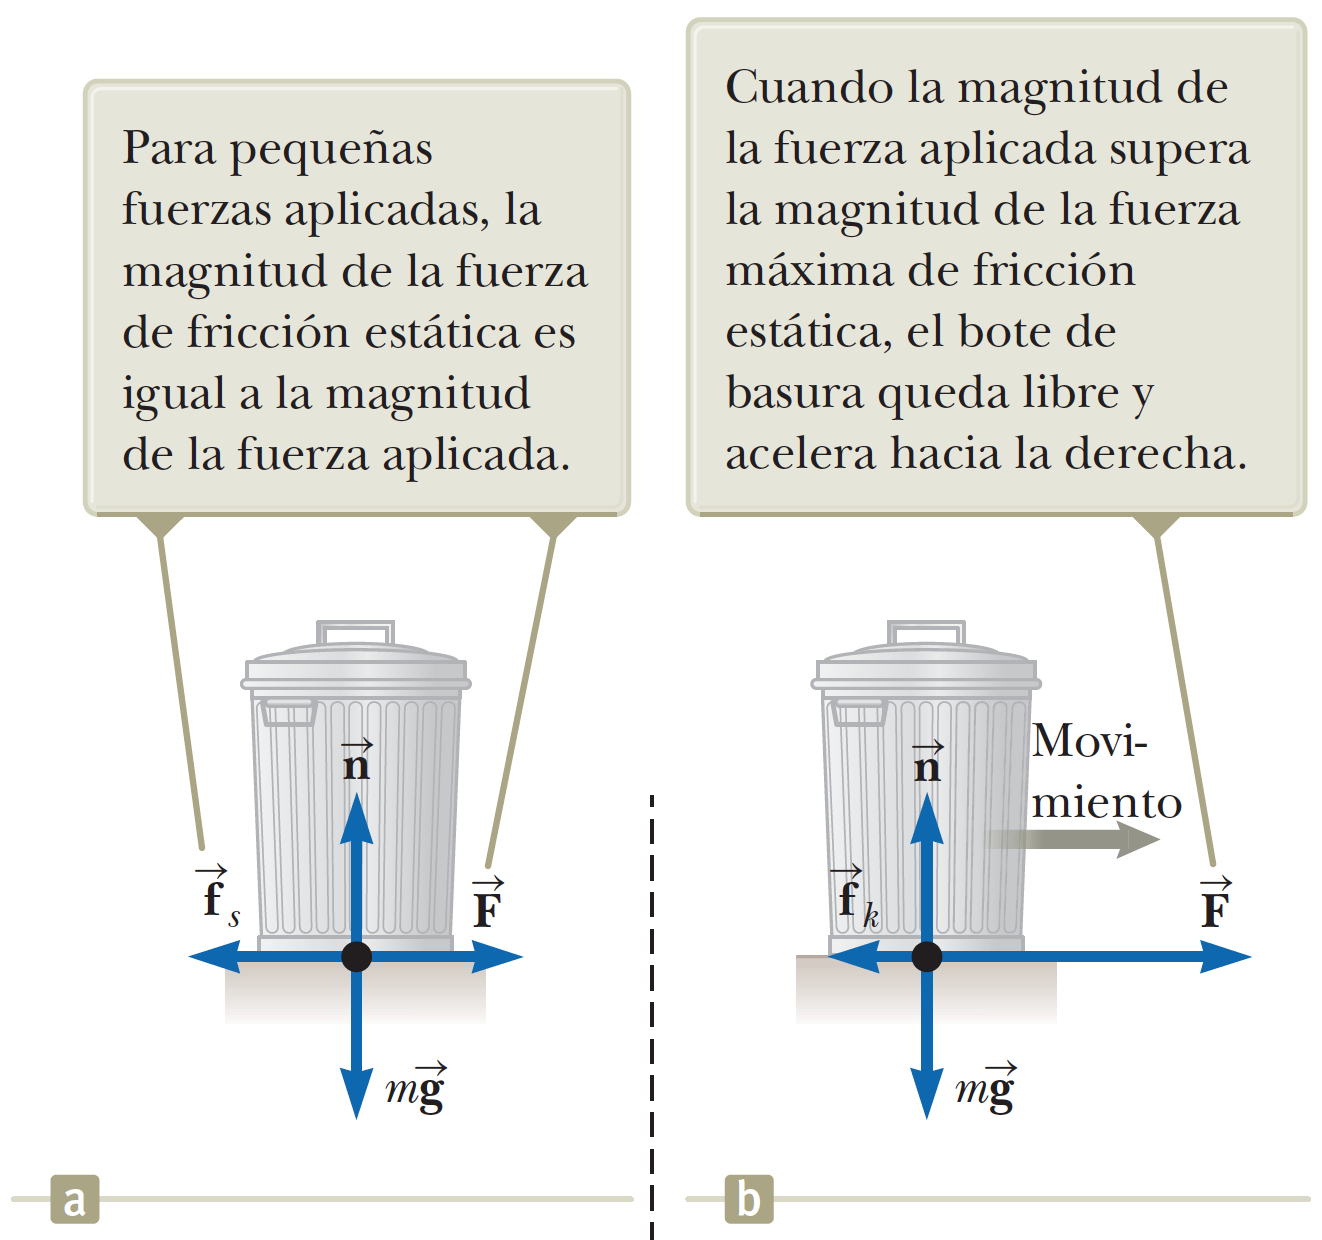
\includegraphics[scale=0.3]{1/graphics_5/figure_4a}
      \caption{Cuando jala un bote de basura, la dirección de la fuerza de fricción $\BV{f}$ entre el bote y una
      superficie rugosa es opuesta a la dirección de la fuerza aplicada $\BV{F}$.}
      \endminipage\hspace{8mm}
      \minipage{0.45\textwidth}
      \centering
      \vspace{18mm}
      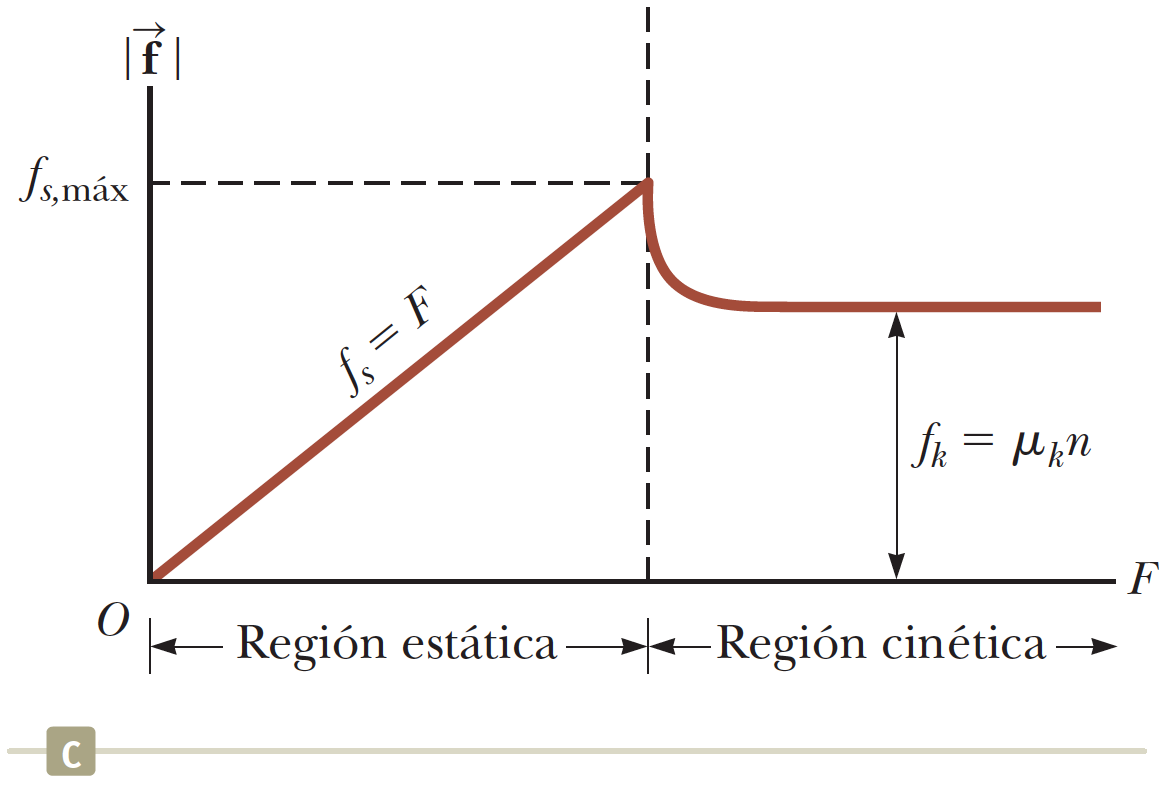
\includegraphics[scale=0.3]{1/graphics_5/figure_4b}
      \caption{Gráfica de fuerza de fricción en función de la fuerza aplicada. Note que $f_{s,max} \geq f_{k}$.}
      \endminipage
    \end{figure}

    \PN A la fuerza de fricción para un objeto en movimiento se le llama \textbf{fuerza de fricción cinética}
    $\BV{f}_{k}$. La fuerza neta $F-f_{k}$ en la dirección $x$ produce una aceleración hacia la derecha, de acuerdo con
    la segunda ley de Newton. Si $F = f_{k}$, la aceleración es cero y el bote de basura se mueve hacia la derecha con
    rapidez constante. Si la fuerza aplicada $\BV{F}$ se elimina del bote en movimiento, la fuerza de fricción
    $\BV{f}_{k}$ que actúa hacia la izquierda proporciona una aceleración del bote de basura en la dirección $-x$ y al
    final lo lleva al reposo.

    \PN Las siguientes descripciones de la fuerza de fricción están en función de las observaciones experimentales y
    sirven como el modelo que se usará para fuerzas de fricción en resolución de problemas:

    \begin{itemize}
      \item La magnitud de la fuerza de fricción estática entre cualesquiera dos superficies en contacto puede tener los
      valores:
        \[
          f_{s} \geq \mu_{s} n
        \]

      \PN donde la constante adimensional $\mu_{s}$ se llama \textbf{coeficiente de fricción estática} y $n$ es la
      magnitud de la fuerza normal que ejerce una superficie sobre la otra. La igualdad se cumple cuando las superficies
      están a punto de deslizarse, esto es, cuando $f_{s} = f_{s, max} = \mu_{s} n$. Esta situación se llama
      \textbf{movimiento inminente}.

      \item La magnitud de la fuerza de fricción cinética que actúa entre dos superficies es:
        \[
          f_{k} = \mu_{k} n
        \]

        \PN donde $\mu_{k}$ se llama \textbf{coeficiente de fricción cinética}. Aunque el coeficiente de fricción
        cinética varía con la rapidez, por lo general en este texto se despreciará cualquiera de tales variaciones.

      \item Los valores de $\mu_{k}, \mu_{s}$ dependen de la naturaleza de las superficies, pero $\mu_{k}$ por lo
      general es menor que $\mu_{s}$.

      \item La dirección de la fuerza de fricción sobre un objeto es paralela a la superficie con la que el objeto está
      en contacto y opuesta al movimiento real (fricción cinética) o al movimiento inminente (fricción estática) del
      objeto en relación con la superficie.

      \item Los coeficientes de fricción son casi independientes del área de contacto entre las superficies.
    \end{itemize}

		\section{Movimiento circular y otras aplicaciones de las leyes de Newton}

		\section{Energía de un sistema}

		\section{Conservación de la energía}

		\section{Cantidad de movimiento lineal y colisiones}
  

		\section{Rotación de un objeto rígido en torno a un eje fijo}

		\section{Cantidad de movimiento angular}

		\section{Equilibrio estático y elasticidad}

		\section{Gravitación universal}


	\part{Movimiento Oscilatorio}
		\subsection{Movimiento de un objeto unido a un resorte}

  \PN \textit{Posición de equilibrio}: Cuando el resorte no está estirado ni comprimido el bloque queda en reposo.

  \vspace{3mm}
  \PN Consideremos el siguiente modelo:

  \begin{figure}[H]
  \centering
    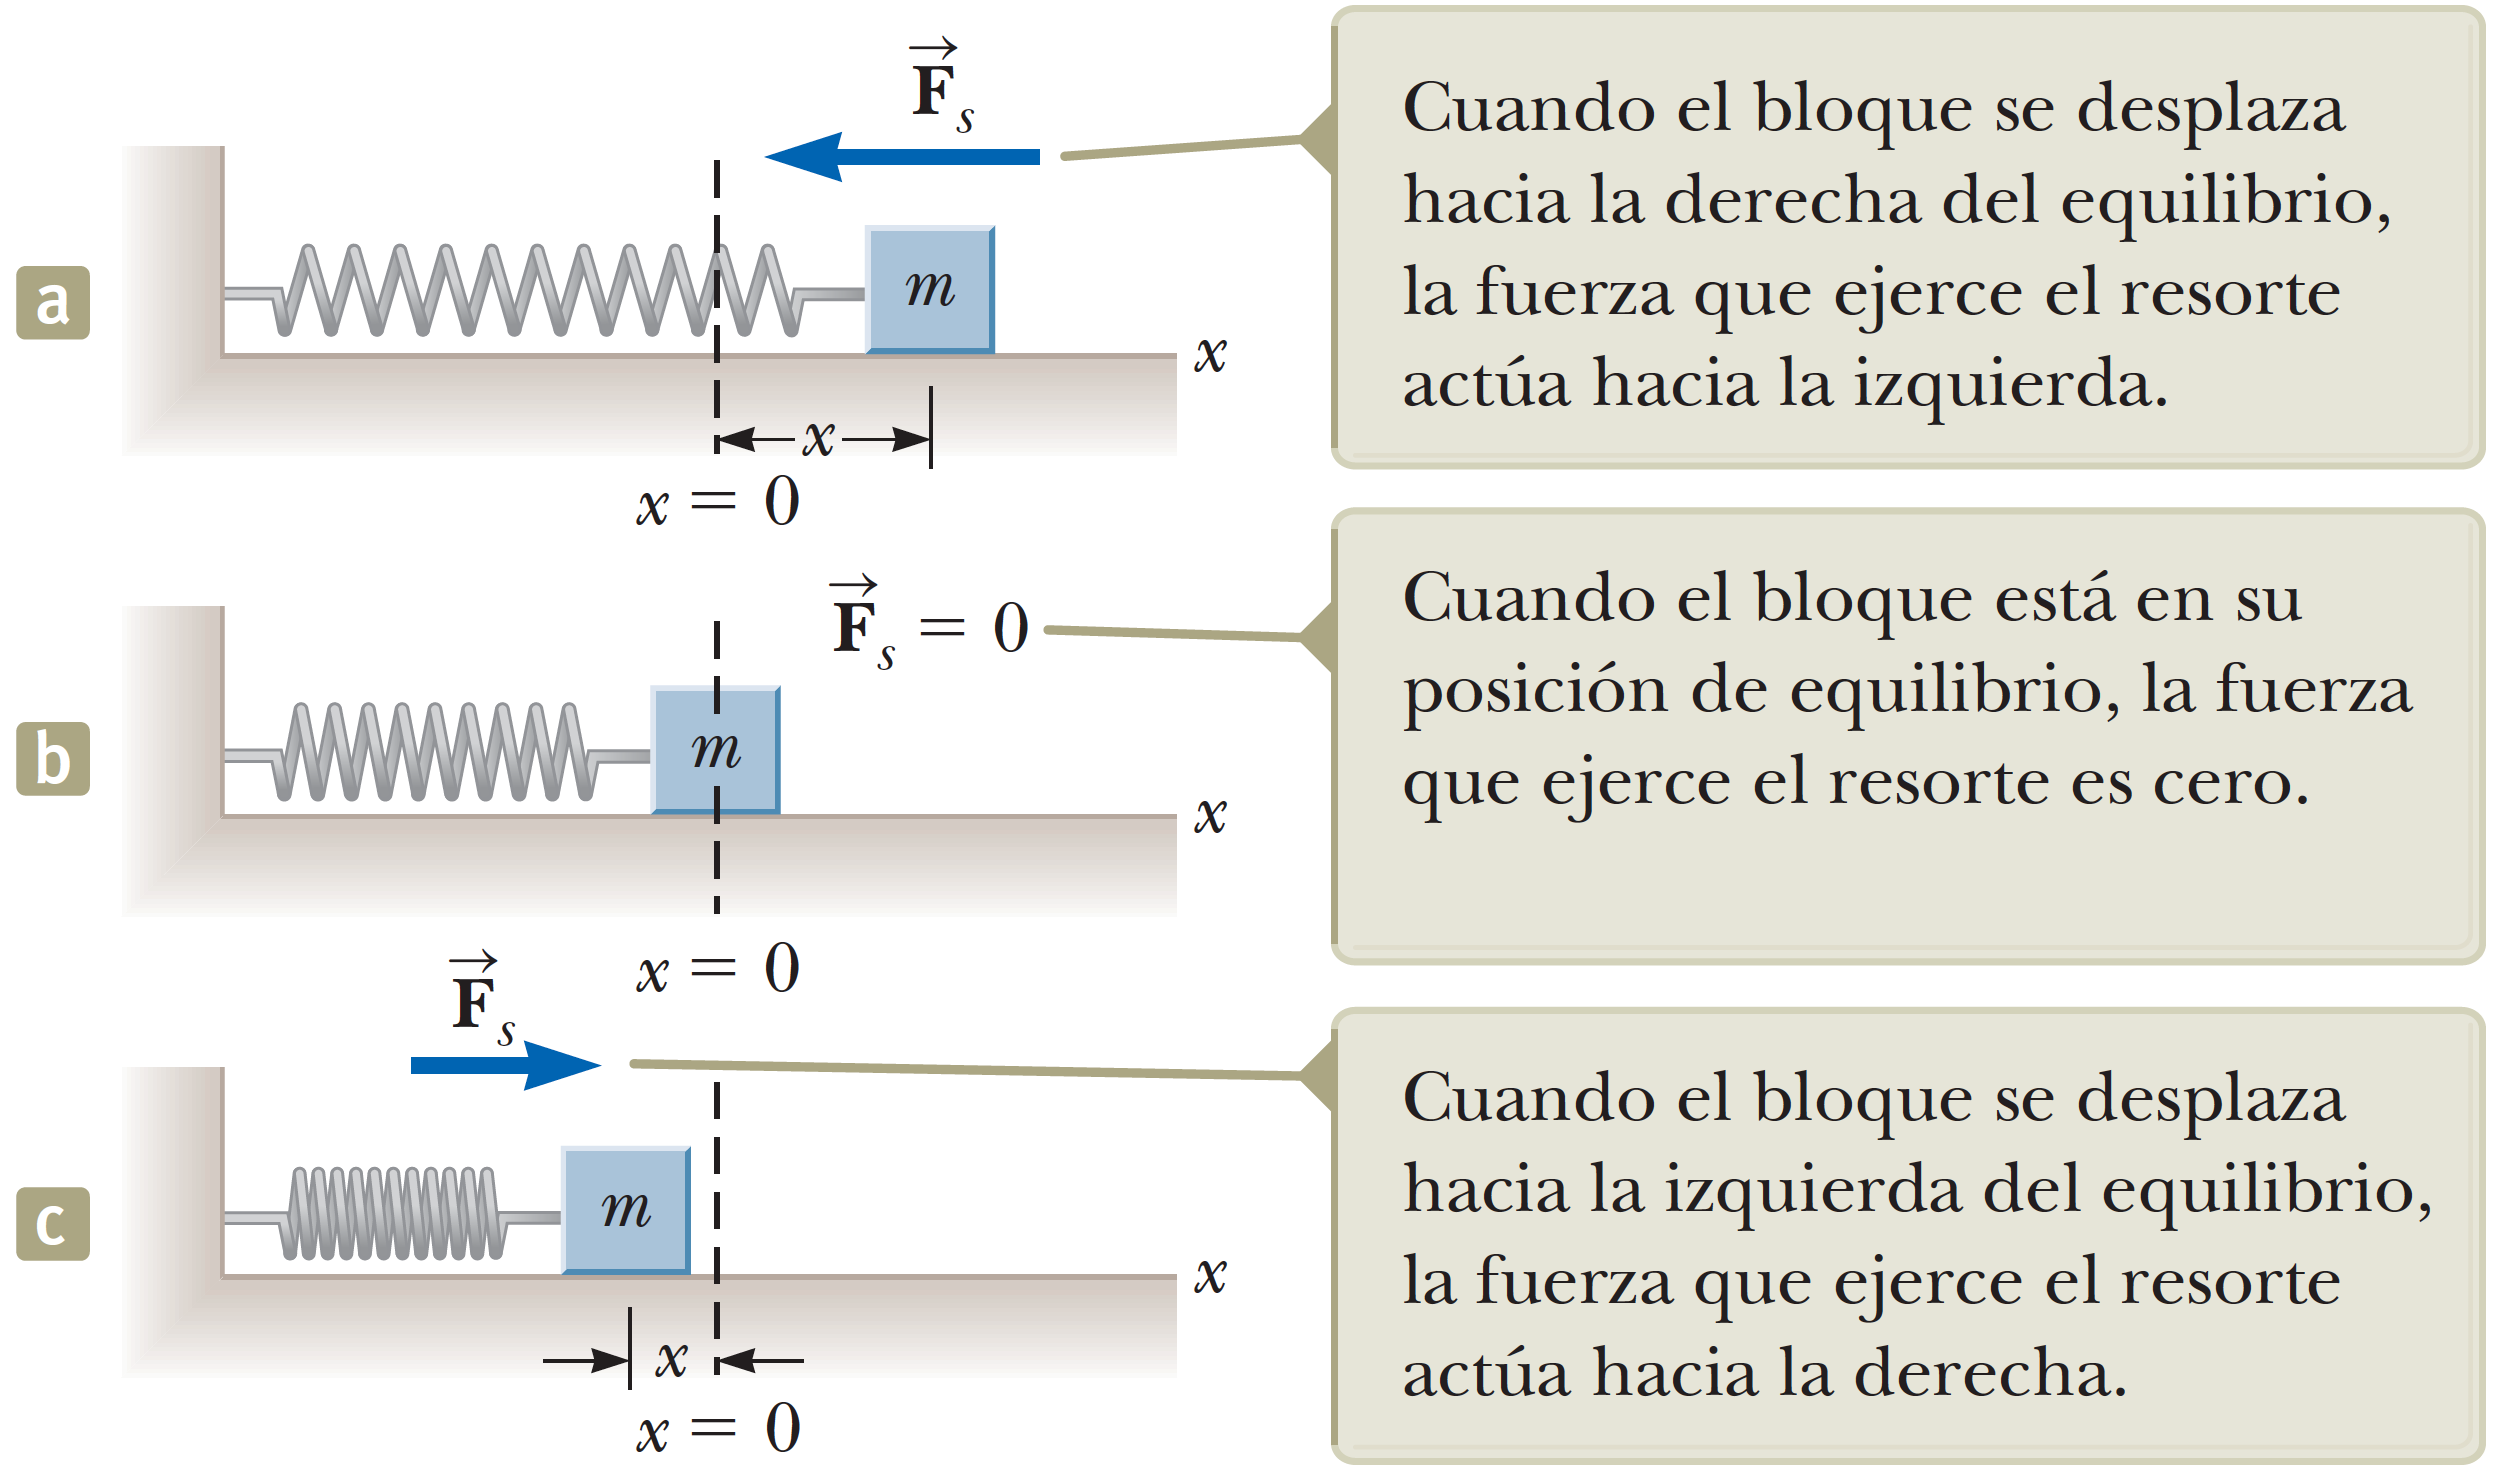
\includegraphics[width=0.6\textwidth]{2/figure_1}
    \caption{Bloque unido a un resorte móvil sobre una superficie sin fricción.}
  \end{figure}

  \PN Cuando el bloque se desplaza a una posición x, el resorte ejerce sobre el bloque una fuerza que es proporcional a
  la posición y está dada por la \textbf{ley de Hooke}:
  \begin{equation}\label{eq:1}
    \underbrace{F_{s}}_{\text{fuerza restauradora}} = -\underbrace{k}_{\text{constante elástica}}\underbrace{x}_{\text{compresión}}
  \end{equation}
  \PN Cuando el bloque es desplazado desde el punto de equilibrio y se suelta, éste es una partícula bajo una fuerza
  neta y, en consecuencia, experimenta una aceleración. Al aplicar la segunda ley de Newton al movimiento del bloque,
  con la ecuación \ref{eq:1} que proporciona la fuerza neta en la dirección x, se obtiene:
  \begin{eqnarray*}
    \Sigma \ F_{x} = ma_{x} &\rightarrow& -kx = ma_{x} \\
    a_{x} &=& \frac{-k}{m}x
  \end{eqnarray*}

  \PN Se dice que los sistemas en los cuales la aceleración del bloque es proporcional a su posición, y la dirección de
  la aceleración es opuesta a la dirección del desplazamiento del bloque desde el equilibrio exhiben \textbf{movimiento
  armónico simple}.

  \PN En ausencia de fricción este movimiento idealizado continuará por siempre porque la fuerza que ejerce el resorte
  es conservativa.

		\subsection{Partícula en movimiento armónico simple}

  \PN La posición de un objeto actuando sobre una fuerza descrita por la \textit{Ley de Hooke} esta dada por:
  \begin{equation}
    x(t) = A \cos (\omega t)
  \end{equation}

  \PN donde A, $\omega$, son constantes y:
  \begin{itemize}
    \item Amplitud del movimiento (A): es simplemente el máximo valor de la posición de la partícula en la dirección x
    positiva o negativa.
    \item Frecuencia angular ($\omega$): es una medida de qué tan rápido se presentan las oscilaciones;
    mientras más oscilaciones por unidad de tiempo haya, más alto es el valor.
    \begin{equation}
      \omega = \sqrt{\frac{k}{m}}
    \end{equation}
    \item Período del movimiento (T): es el intervalo de tiempo requerido para que la partícula pase a través de un
    ciclo completo de su movimiento.
    \begin{equation}
      T = \frac{2\pi}{\omega} = 2\pi \sqrt{\frac{m}{k}}
    \end{equation}
    \item Frecuencia (f): representa el número de oscilaciones que experimenta la partícula por unidad de intervalo de
    tiempo.
    \begin{equation}
      f = \frac{1}{T} = \frac{1}{2\pi} \sqrt{\frac{k}{m}}
    \end{equation}
  \end{itemize}

  \PN \textbf{Ecuaciones de velocidad y de aceleración}
  \begin{eqnarray*}
    v = \frac{dx}{dt} &=& - \omega A \sin (\omega t) \\
    a = \frac{d^{2}x}{dt^{2}} &=& - \omega^{2} A \cos (\omega t)
  \end{eqnarray*}

  \PN \textbf{Valores máximos}
  \begin{eqnarray*}
    x_{max} &=& A \\
    v_{max} &=& \omega A = \sqrt{\frac{k}{m}} \\
    a_{max} &=& \omega^{2} A = \frac{k}{m} A
  \end{eqnarray*}

		\subsection{Energía del oscilador armónico simple}

\PN \textbf{Energía cinética}
\begin{equation}
  K = \frac{1}{2} m v^{2} = \frac{1}{2} m \omega^{2} A^{2} \sin^{2} (\omega t)
\end{equation}

\PN \textbf{Energía potencial}
\begin{equation}
  U = \frac{1}{2} k x^{2} = \frac{1}{2} k A^{2} \cos^{2} (\omega t)
\end{equation}

\PN \textbf{Energía total}
\PN Dado que K y U siempre son cantidades positivas o cero. Puesto que $\omega^{2} = \frac{k}{m}$, la energía mecánica
total del oscilador armónico simple se expresa como:
\begin{eqnarray*}
  E &=& K + U = \frac{1}{2} k A^{2} [\sin^{2} (\omega t) + \cos^{2} (\omega t)] \\
  &=& \frac{1}{2} k A^{2}
\end{eqnarray*}

\pagebreak
\PN \textbf{Velocidad como una función de la posición}
\PN La velocidad del bloque en una posición arbitraria se obtiene al expresar la energía total del sistema en alguna
posición arbitraria x como:
\begin{eqnarray*}
  E &=& K + U = \frac{1}{2} m v^{2} + \frac{1}{2} k x^{2} = \frac{1}{2} k A^{2} \\
  v &=& \pm \sqrt{\frac{k}{m} (A^{2} - x^{2})} = \pm \omega \sqrt{A^{2} - x^{2}}
\end{eqnarray*}

		\subsection{Osciladores amortiguados}

  \PN En muchos sistemas reales, fuerzas no conservativas como la fricción o la resistencia del aire retardan el
  movimiento del sistema. En consecuencia, la energía mecánica del sistema disminuye en el tiempo y se dice que el
  movimiento está amortiguado.

  \vspace{3mm}
  \PN Consideremos el siguiente modelo:

  \begin{figure}[H]
  \centering
    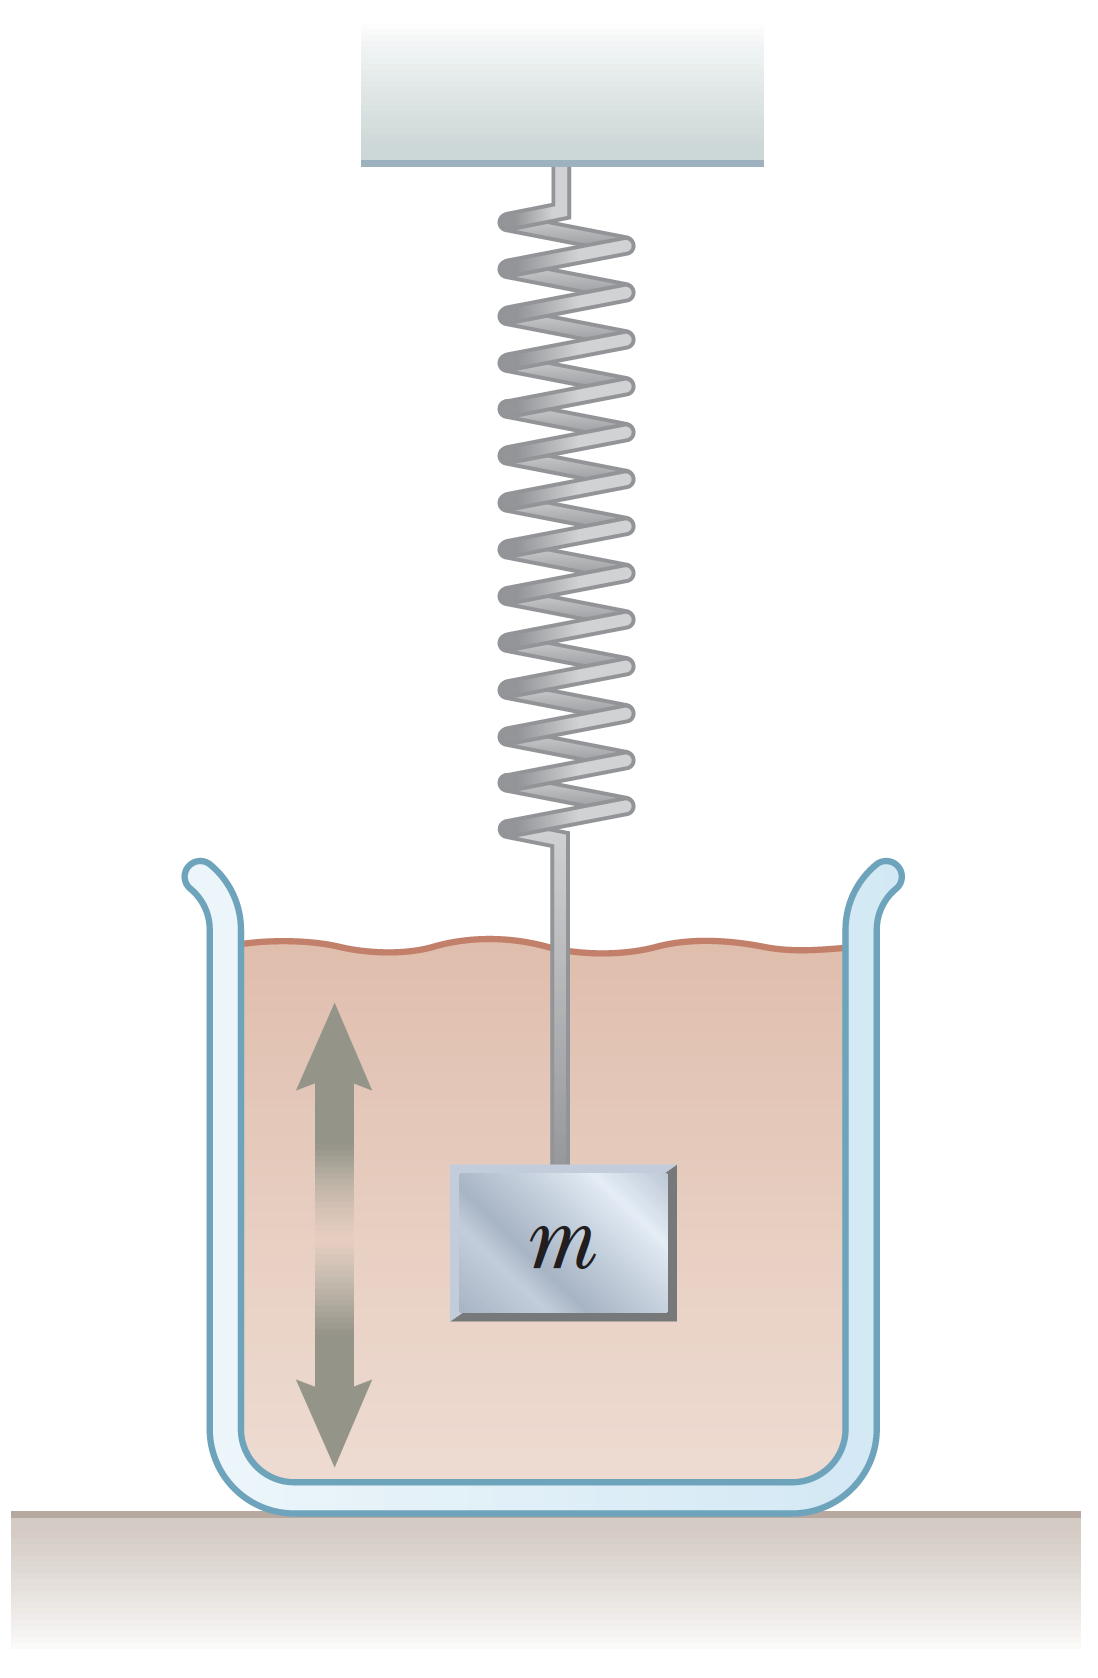
\includegraphics[width=0.15\textwidth]{2/figure_2}
    \caption{Ejemplo de un oscilador amortiguado es un objeto unido a un resorte y sumergido en un líquido viscoso.}
  \end{figure}

  \PN Se puede escribir la segunda ley de Newton como:
  \begin{eqnarray*}
    \Sigma \ F_{x} &=& -kx - \underbrace{b \overbrace{v}^{\text{coeficiente de amortiguamiento}}}_{\text{fuerza retardadora}} = ma_{x} \\
    -kx - b \frac{dx}{dt} &=& m \frac{d^{2}x}{dt^{2}}
  \end{eqnarray*}

  \PN \textbf{Ecuación de la posición}
  \begin{equation}
    x(t) = A \mathrm{e}^{\frac{-b}{2m}t} \cos (\omega t)
  \end{equation}

  \PN donde la frecuencia angular de oscilación es:
  \begin{equation}
    \omega = \sqrt{\frac{k}{m} - \left(\frac{b}{2m}\right)^{2}}
  \end{equation}

  \PN Es conveniente expresar la frecuencia angular de un oscilador amortiguado en la forma:
  \begin{equation}
    \omega = \sqrt{\omega_{0} - \left(\frac{b}{2m}\right)^{2}}
  \end{equation}

  \PN donde $\omega_{0} = \sqrt{k/m}$ representa la frecuencia angular en ausencia de una fuerza retardadora (el
  oscilador no amortiguado) y se llama \textbf{frecuencia natural} del sistema.

  \pagebreak
  \PN \textbf{Tipos de amortiguamiento}
  \begin{itemize}
    \item Subamortiguado: $\omega_{0} > \frac{b}{2m}$
    \item Críticamente Amortiguado: $\omega_{0} = \frac{b}{2m}$
    \item Sobreamortiguado: $\omega_{0} < \frac{b}{2m}$
  \end{itemize}

		\subsection{Oscilaciones forzadas}

  \PN Se ha visto que la energía mecánica de un oscilador amortiguado disminuye en el tiempo como resultado de la fuerza
  retardadora. Es posible compensar esta disminución de energía al aplicar una fuerza externa que haga trabajo positivo
  sobre el  sistema. En cualquier instante se puede transferir energía al sistema mediante una fuerza aplicada que actúe
  en la dirección de movimiento del oscilador.

  \PN Al modelar un oscilador con fuerzas retardadoras e impulsoras como una partícula bajo una fuerza neta, la segunda
  ley de Newton en esta situación produce:
  \begin{equation}
    \Sigma \ F_{x} = ma_{x} \rightarrow F_{0} \sin (\omega t) -b \frac{dx}{dt} - kx = m \frac{d^{2}x}{dt^{2}}
  \end{equation}

  \PN \textbf{Ecuación de la posición}
  \begin{equation}
    x(t) = A \cos (\omega t)
  \end{equation}

  \PN donde
  \begin{equation}
    A = \frac{F_{0}/m}{\sqrt{\left(\omega^{2} - \omega_{0}^{2}\right)^{2} - \left(\frac{b\omega}{m}\right)^{2}}}
  \end{equation}

  \PN y donde $\omega_{0} = \sqrt{k/m}$ es la frecuencia natural del oscilador subamortiguado ($b = 0$).


	\part{Termodinámica}
		\subsection{Temperatura y ley cero de la termodinámica}

  \PN \underline{Contacto térmico:} dos objetos están en contacto térmico mutuo si entre ellos pueden intercambiar
  energía mediante dichos procesos debido a una diferencia de temperatura.

  \vspace{3mm}
  \PN \underline{Equilibrio térmico:} es una situación en la que dos objetos no intercambian energía, por calor o por
  radiación electromagnética, si se colocan en contacto térmico.

  \vspace{3mm}
  \PN \textbf{Ley cero de la termodinámica}
  \PN Si dos objetos A y B están por separado en equilibrio térmico con un tercer objeto C, entonces A y B están en
  equilibrio térmico entre sí.

  \vspace{3mm}
  \PN \underline{Temperatura:} propiedad que determina si un objeto está en equilibrio térmico con otros objetos.

		\subsection{Termómetros y escala de temperatura Celsius}

  \PN \underline{Termométro:} son dispositivos que sirven para medir la temperatura de un sistema.

  \vspace{3mm}
  \PN El termómetro se calibra al colocarlo en contacto térmico con un sistema natural que permanezca a temperatura
  constante. Uno de dichos sistemas es una mezcla de hielo y agua en equilibrio térmico a presión atmosférica. En la
  \textbf{escala de temperatura Celsius}, esta mezcla se define que tiene una temperatura de cero grados Celsius, que se
  escribe como $0º$C; esta temperatura se llama \textit{punto de hielo del agua}. Otro sistema empleado comúnmente es
  una mezcla de agua y vapor en equilibrio térmico a presión atmosférica; su temperatura se define como $100º$C, que es
  el \textit{punto de vapor del agua}.

		\subsection{Escala absoluta de temperatura}

  \PN \underline{Cero absoluto:} se establece al valor $-273.15º$C para la \textbf{escala absoluta de temperatura}.

  \vspace{3mm}
  \PN El tamaño de un grado en la escala absoluta de temperatura se elige como idéntica al tamaño de un grado en la
  escala Celsius. Por lo tanto, la conversión entre dichas temperaturas es:
  \begin{equation*}
    T_{C} = T - 273.15
  \end{equation*}

  \PN donde $T_{C}$ es la temperatura Celsius y T es la temperatura absoluta.

  \vspace{3mm}
  \PN \textbf{Las escalas de temperatura Celsius, Fahrenheit y Kelvin}
  \PN La \textit{escala Fahrenheit} ubica la temperatura del punto de hielo en $32º$F y la temperatura del punto de
  vapor en $212º$F. La relación entre las escalas de temperatura Celsius y Fahrenheit es:
  \begin{equation*}
    T_{F} = \frac{9}{5} T_{C} + 32º F
  \end{equation*}

  \PN La relación entre los cambios de temperatura en las escalas Celsius, Kelvin y Fahrenheit:
  \begin{equation*}
    \Delta T_{C} = \Delta T = \frac{5}{9} \Delta T_{F}
  \end{equation*}

  \PN De estas tres escalas de temperatura, sólo la escala Kelvin se apoya en un verdadero valor cero de temperatura.

		\subsection{Expansión térmica de sólidos y líquidos}

  \PN El estudio del termómetro líquido utiliza uno de los cambios mejor conocidos en una sustancia: a medida que
  aumenta su temperatura, su volumen se incrementa. Este fenómeno, conocido como \textbf{expansión térmica}, desempeña
  un importante papel en numerosas aplicaciones de ingeniería. La expansión térmica es una consecuencia del cambio en la
  separación promedio entre los átomos en un objeto.

  \PN Suponga que un objeto tiene una longitud inicial $L_{i}$ a lo largo de alguna dirección en alguna temperatura, y
  la longitud aumenta en una cantidad $\Delta L$ para un cambio en temperatura $\Delta T$. Es conveniente considerar el
  cambio fraccionario en longitud por cada grado de cambio de temperatura, entonces se define el \textit{coeficiente de
  expansión lineal} promedio como:
  \begin{equation*}
    \alpha \equiv \frac{\Delta L / L_{i}}{\Delta T}
  \end{equation*}

  \PN Para fines de cálculo, esta ecuación se reescribe como:
  \begin{equation*}
    \Delta L = \alpha L_{i} \Delta T
  \end{equation*}

  \PN o en la forma:
  \begin{equation*}
    L_{f} - L_{i} = \alpha L_{i} \left(T_{f} - T_{i}\right)
  \end{equation*}

  \PN donde $L_{f}$ es la longitud final, $T_{i}$ y $T_{f}$ son las temperaturas inicial y final, respectivamente, y la
  constante de proporcionalidad a es el coeficiente de expansión lineal promedio para un material dado y tiene unidades
  de $(ºC)^{-1}$.

  \PN Ya que las dimensiones lineales de un objeto cambian con la temperatura, se sigue que el área superficial y el
  volumen cambian. El cambio en volumen es proporcional al volumen inicial $V_{i}$ y al cambio en temperatura de acuerdo
  con la relación:
  \begin{equation*}
    \Delta V = \beta V_{i} \Delta T
  \end{equation*}

  \PN Comunmente, se cumple que $\beta = 3 \alpha$.

		\subsection{Descripción macroscópica de un gas ideal}

  \PN La ecuación de expansión volumétrica $\Delta V = \beta V_{i} \Delta T$ se basa en la suposición de que el material
  tiene un volumen inicial $V_{i}$ antes de que ocurra un cambio de temperatura. Tal es el caso para sólidos y líquidos,
  porque tienen un volumen fijo a una temperatura dada.

  \PN Para un gas, es útil saber cómo se relacionan las cantidades volumen $V$, presión $P$ y temperatura $T$ para una
  muestra de gas de masa $m$. En general, la ecuación que interrelaciona estas cantidades, llamada \textit{ecuación de
  estado}, es muy complicada. Sin embargo, si el gas se mantiene a una presión muy baja (o densidad baja), la ecuación
  de estado es muy simple y se puede determinar a partir de resultados experimentales. Tal gas de densidad baja se
  refiere como un gas ideal. El modelo de gas ideal se puede emplear para efectuar predicciones que sean adecuadas para
  describir el comportamiento de gases reales a bajas presiones.

  \vspace{3mm}
  \PN \textbf{Ley de gas ideal}
  \begin{equation*}
    P V = c T
  \end{equation*}

  \PN donde c, es una constante que se define como $c = nR$, con $n$ el número de \textit{moles} de la sustancia y $R$
  se llama \textbf{constante universal de los gases} y tiene el valor:
  \begin{equation*}
    R = 0.082 \; \frac{L \; atm}{mol \; K}
  \end{equation*}

		\subsection{Calor y energía interna}
  \PN La \textbf{energía interna} es toda la energía de un sistema que se asocia con sus componentes microscópicos,
  átomos y moléculas, cuando se observa desde un marco de referencia en reposo respecto al centro de masa del sistema.

  \vspace{3mm}
  \PN El \textbf{calor} se define como un proceso de transferencia de energía a través de la frontera de un sistema
  debido a una diferencia de temperatura entre el sistema y sus alrededores. También es la cantidad de energía Q
  transferida mediante este proceso.

  \vspace{3mm}
  \PN La \textbf{caloría} (cal), que se define como la cantidad de transferencia de energía necesaria para elevar legal
  temperatura de 1 $g$ de agua de $14.5º$C a $15.5º$C.

  \vspace{3mm}
  \PN \textbf{Equivalente mécanico del calor}
  \begin{equation*}
    1 \; \text{cal} = 4.186 \; \text{J}
  \end{equation*}

  \PN Un nombre más conveniente sería \textit{equivalencia entre energía mecánica y energía interna}, pero el nombre
  histórico tiene mucha presencia en el lenguaje cotidiano, a pesar del uso incorrecto de la palabra calor.

		\subsection{Calor específico y calorimetría}

  \PN La \textbf{capacidad térmica} (o calorífica) C de una muestra particular se define como la cantidad de energía
  necesaria para elevar la temperatura de dicha muestra en $1º$C. A partir de esta definición, se ve que si la energía
  $Q$ produce un cambio $\Delta T$ en la temperatura de una muestra, entonces
  \begin{equation*}
    Q = C \Delta T = C (T_{f} - T_{i})
  \end{equation*}

  \PN El \textbf{calor específico} $c$ de una sustancia es la capacidad térmica por unidad de masa. Por lo tanto, si a
  una muestra de una sustancia con masa $m$ se le transfiere energía $Q$ y la temperatura de la muestra cambia en
  $\Delta T$, el calor específico de la sustancia es:
  \begin{equation*}
    c \equiv \frac{Q}{m \Delta T} \qquad \text{i.e} \qquad C = mc
  \end{equation*}

  \PN donde
  \begin{equation*}
    \left[c\right] = \frac{\text{cal}}{\text{g} º\text{C}} = 4.186 \frac{\text{J}}{\text{kg K}}
  \end{equation*}

  \PN El calor específico es en esencia una medida de qué tan insensible térmicamente es una sustancia a la adición de
  energía.

  \vspace{3mm}
  \PN A partir de esta definición, es factible relacionar la energía $Q$ transferida entre una muestra de masa $m$ de un
  material y sus alrededores con un cambio de temperatura $\Delta T$ como:
  \begin{equation*}
    Q = mc \Delta T
  \end{equation*}

		\subsection{Calor latente}

  \PN \underline{Convención:} se utilizará el término \textit{material de fase superior} para indicar que el material
  está a una temperatura alta, cuando se estudien dos fases de un material.

  \vspace{3mm}
  \PN Considere un sistema que contiene una sustancia en dos fases en equilibrio, como hielo y agua. La cantidad inicial
  de material de fase superior, agua, en el sistema es $m_{i}$. Ahora imagine que al sistema entra la energía Q. Como
  resultado, la cantidad final de agua es $m_{f}$ debido a la fusión de un poco de hielo. Por lo tanto, la cantidad de
  hielo derretido es igual a la cantidad de agua nueva: $\Delta m = m_{f} - m_{i}$. Para este cambio de fase, el calor
  latente se define como:
  \begin{equation*}
    \text{L} \equiv \frac{\text{Q}}{\Delta m}
  \end{equation*}

  \PN De la definición de calor latente, y de nuevo al elegir el calor como el mecanismo de transferencia de energía, la
  energía requerida para cambiar la fase de una sustancia pura es:
  \begin{equation*}
    \text{Q} = \text{L} \; \Delta m
  \end{equation*}

  \PN donde $\Delta m$ es el cambio en masa del material de fase superior.

  \begin{itemize}
    \item \textbf{Calor latente de fusión} ($L_{f}$): es el término que se aplica cuando el cambio de fase es de sólido
    a líquido.
    \item \textbf{Calor latente de vaporización:} ($L_{v}$): es el término que se usa cuando el cambio de fase es de
    líquido a gas.
  \end{itemize}

		\subsection{Mecanismos de transferencia de energía en procesos térmicos}

  \PN El proceso de transferencia de energía por calor también se llama \textbf{conducción} o \textbf{conducción
  térmica}.

  \vspace{3mm}
  \PN Consideremos el siguiente modelo:
  \begin{figure}[H]
  \centering
    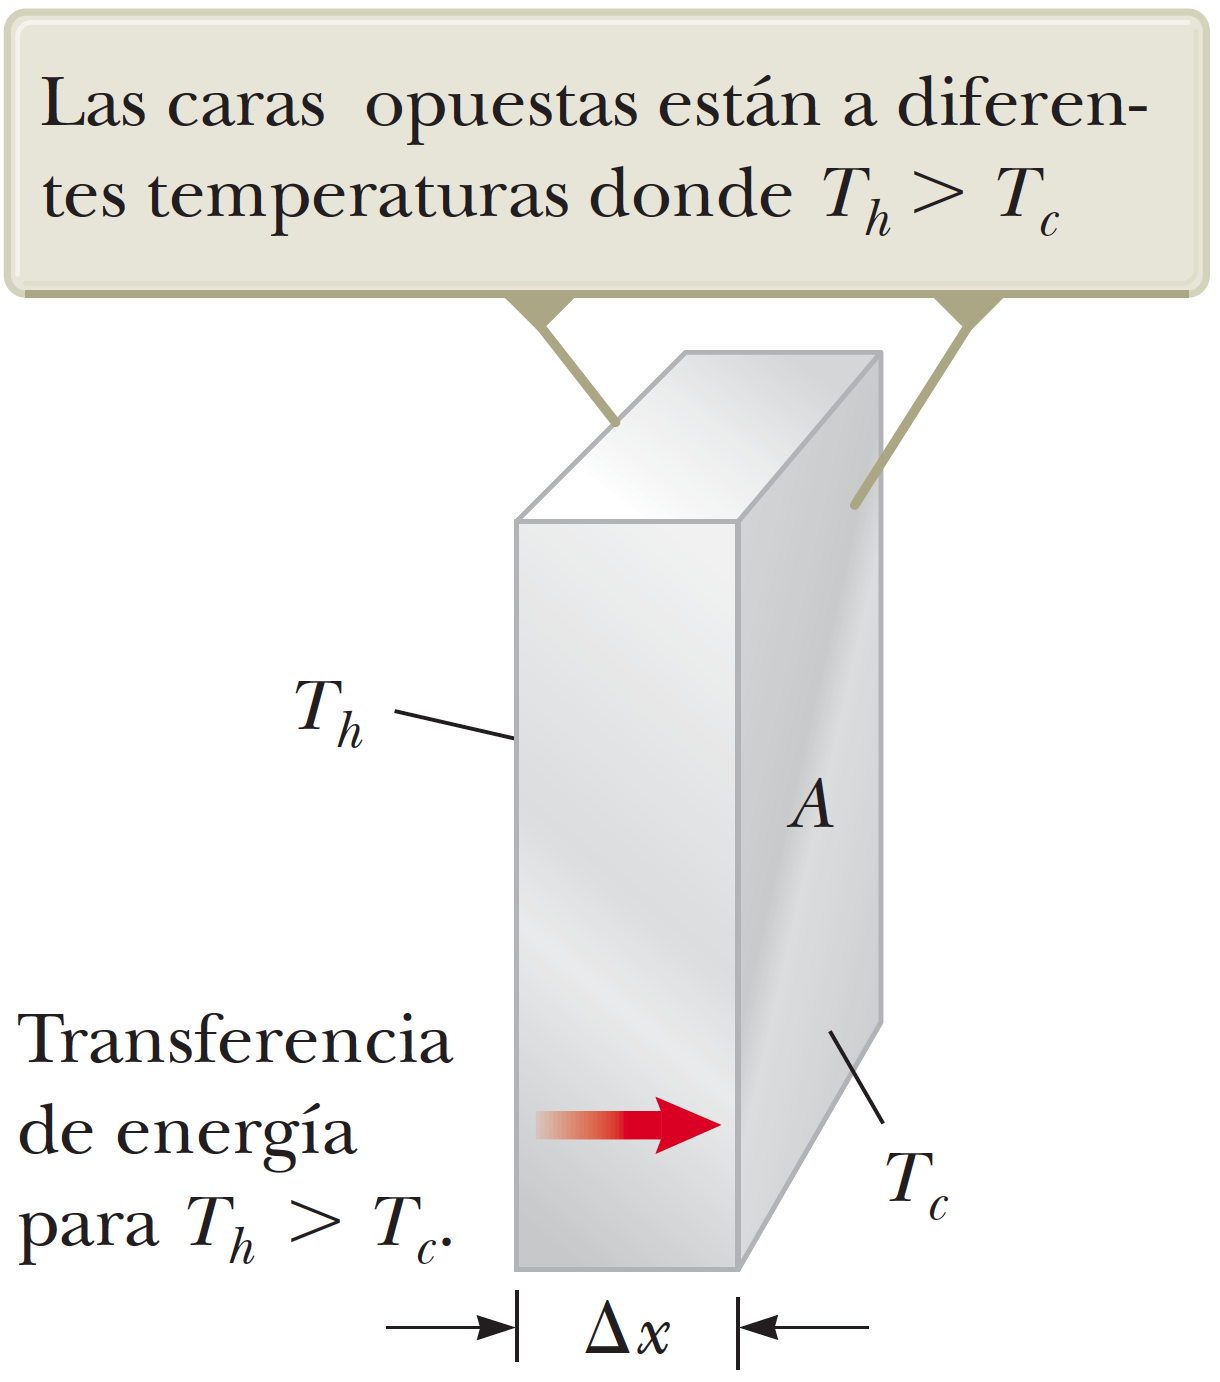
\includegraphics[width=0.3\textwidth]{3/figure_1}
    \caption{Transferencia de energía a través de una placa conductora con un área de sección transversal A y un espesor
    $\Delta x$.}
  \end{figure}

  \PN La conducción se presenta sólo si hay una diferencia en temperatura entre dos partes del medio de conducción.
  Considere una placa de material de espesor $\Delta x$ y área de sección transversal A. Una cara de la placa está a una
  temperatura $T_{c}$ y la otra está a una temperatura $T_{h} > T_{c}$. Se encuentra que la energía Q se transfiere en
  un intervalo de tiempo $\Delta t$ desde la cara más caliente hacia la más fría. La rapidez $P = \text{Q} / \Delta t$ a
  la que ocurre esta transferencia de energía se encuentra que es proporcional al área de sección transversal y a la
  diferencia de temperatura $\Delta T = T_{h} - T_{c}$, e inversamente proporcional al espesor:
  \begin{equation*}
    \text{P} = \frac{\text{Q}}{\Delta t} \propto \text{A} \frac{\Delta \text{T}}{\Delta x}
  \end{equation*}

  \PN Para una placa de espesor infinitesimal $dx$ y diferencia de temperatura $dT$, se escribe la \textbf{ley de
  conducción térmica} como:
  \begin{equation*}
    \text{P} = k \text{A} \abs{\frac{d\text{T}}{dx}}
  \end{equation*}

  \PN donde la constante de proporcionalidad $k$ es la conductividad térmica del material y $\abs{\frac{dT}{dx}}$ es el
  gradiente de temperatura.

  \vspace{3mm}
  \PN Suponga que una larga barra uniforme de longitud L se aísla térmicamente de modo que la energía no puede escapar
  por calor de su superficie, excepto en los extremos. Un extremo está en contacto térmico con un depósito de energía a
  temperatura $T_{c}$, y el otro extremo está en contacto térmico con un depósito a temperatura $T_{h} > T_{c}$. Cuando
  se logra un estado estable, la temperatura en cada punto a lo largo de la barra es constante en el tiempo. En este
  caso, si se supone que $k$ no es una función de la temperatura, el gradiente de temperatura es el mismo en todas
  partes a lo largo de la barra y es:
  \begin{equation*}
    \abs{\frac{d\text{T}}{dx}} = \frac{\text{T}_{h} - \text{T}_{c}}{\text{L}}
  \end{equation*}

  \PN Por lo tanto, la rapidez de transferencia de energía por conducción a través de la barra es:
  \begin{equation*}
    \text{P} = \frac{k\text{A}}{\text{L}} \left(\text{T}_{h} - \text{T}_{c}\right)
  \end{equation*}

  \PN \textbf{Resistencia térmica}
  \PN El término L/$k$ para una sustancia particular se conoce como el valor R del material. Por lo tanto
  \begin{equation*}
    \text{P} = \frac{\text{A} \left(\text{T}_{h} - \text{T}_{c}\right)}{\sum_{i} R_{i}}
  \end{equation*}

  \PN donde $R_{i} = \text{L}_{i} / k_{i}$.

  \vspace{3mm}
  \PN \textbf{Convección}
  \PN Se dice que la energía transferida por el movimiento de una sustancia caliente se transfiere por convección, que
  es una forma de transferencia de materia.
  \begin{equation*}
    \text{P} = h \text{A} \left(\text{T} - \text{T}_{0}\right)
  \end{equation*}

  \PN donde $h$ es la \textit{constante de convección}, A es la \textit{superficie de contacto} y T es la
  \textit{temperatura del cuerpo}.

  \vspace{3mm}
  \PN \textbf{Radiación}
  \PN El tercer medio de transferencia de energía que se analizará es la \textbf{radiación térmica}.
  \PN La rapidez a la que un objeto radia energía es proporcional a la cuarta potencia de la temperatura absoluta de la
  superficie. Conocida como ley de Stefan, este comportamiento se expresa en forma de ecuación como:
  \begin{equation*}
    \text{P} = \sigma \text{A} e \text{T}^{4}
  \end{equation*}

  \PN donde P es la potencia en watts de las ondas electromagnéticas radiadas de la superficie del objeto, $\sigma$ es
  una constante igual a $5.67$ x $10^{-8} \; W/m^{2} K^{4}$, A es el área superficial del objeto en metros cuadrados,
  $e$ es la emisividad y T es la temperatura superficial en kelvins.

  \PN Si un objeto está a una temperatura T y sus alrededores están a una temperatura promedio T$_{0}$, la rapidez neta
  de energía ganada o perdida por el objeto como resultado de la radiación es:
  \begin{equation*}
    \text{P}_{neta} = \sigma \text{A} e \left(\text{T}^{4} - \text{T}_{0}^{4}\right)
  \end{equation*}


	\part{Electricidad y magnetismo}
		\section{Campos eléctricos}

  \subsection{Propiedades de las cargas eléctricas}
    \PN Propiedades:
    \begin{itemize}
      \item existen dos tipos de cargas eléctricas, \textit{positiva} y \textit{negativa}.
      \item cargas de un mismo signo se repelen y cargas de signos opuestos se atraen.
      \item en un sistema aislado la carga eléctrica siempre se conserva.
      \item las cargas eléctricas siempre se presentan como un entero múltiplo de una cantidad básica de carga $e$.
      \item la carga eléctrica se escribe $q = \pm Ne$ donde $N$ es algún número entero.
      \item el electrón tiene una carga $-e$ y el protón una carga $+e$. El neutrón, no posee carga.
    \end{itemize}

  \subsection{Objetos de carga mediante inducción}
    \begin{itemize}
      \item Los \textbf{conductores} eléctricos son aquellos materiales en los cuales algunos de los electrones son
      libres no están unidos a átomos y pueden moverse con libertad a través del material.
      \item Los \textbf{aislantes} eléctricos son aquellos materiales en los cuales todos los electrones están unidos a
      átomos y no pueden moverse libremente a través del material.
      \item Los \textbf{semiconductores}, tienen propiedades eléctricas que se ubican entre las correspondientes a los
      aislantes y a los conductores.
    \end{itemize}

  \subsection{Ley de Coulomb}
    \PN Al generalizar las propiedades de la fuerza eléctrica entre dos partículas inmóviles con carga, se usa el
    término \textit{carga puntual} que hace referencia a una partícula con carga de tamaño cero.

    \PN Debido a observaciones experimentales es posible encontrar la magnitud de una fuerza eléctrica entre dos cargas
    puntuales establecidas por la \textbf{Ley de Coulomb}:
    \begin{equation*}
      F = k \ \frac{\abs{q_{1}} \abs{q_{2}}}{r^{2}}
    \end{equation*}

    \PN donde k es una constante conocida como constante de Coulomb.

    \PN La fuerza eléctrica, como la fuerza de gravedad, es conservativa.

    \PN La unidad de carga del SI es el \textbf{coulomb (C)}. La constante de Coulomb k en unidades del SI tiene el
    valor:
    \begin{equation*}
      k = 8.987 \ \text{x} \ 10^{9} \ \frac{\text{N} m^{2}}{\text{C}^{2}}
    \end{equation*}

    \PN Además esta constante se expresa como:
    \begin{equation*}
      k = \frac{1}{4 \pi \varepsilon_{0}}
    \end{equation*}

    \PN donde la constante $\varepsilon_{0}$ se conoce como la \textit{permitividad del vacío}, cuyo valor es:
    \begin{equation*}
      \varepsilon_{0} = 8.8542 \ \text{x} \ 10^{-12} \ \frac{\text{C}^{2}}{\text{N} m^{2}}
    \end{equation*}

    \PN La unidad de carga más pequeña, es la carga de un electrón ($-e$) o de un protón ($e$), con una magnitud de:
    \begin{equation*}
      e = 1.60218 \ \text{x} \ 10^{-19} \text{C}
    \end{equation*}

    \PN La ley de Coulomb, expresada en forma vectorial para una fuerza eléctrica ejercida por una carga $q_{1}$ sobre
    una segunda carga $q_{2}$, rescrita como $\vec{F}_{12}$, es
    \begin{equation*}
      \vec{F}_{12} = k \ \frac{q_{1} q_{2}}{r^{2}} \ \hat{r}_{12}
    \end{equation*}

    \PN donde $\hat{r}_{12}$ es un vector unitario dirigido de $q_{1}$ hacia $q_{2}$.
    \begin{figure}[H]
    \centering
      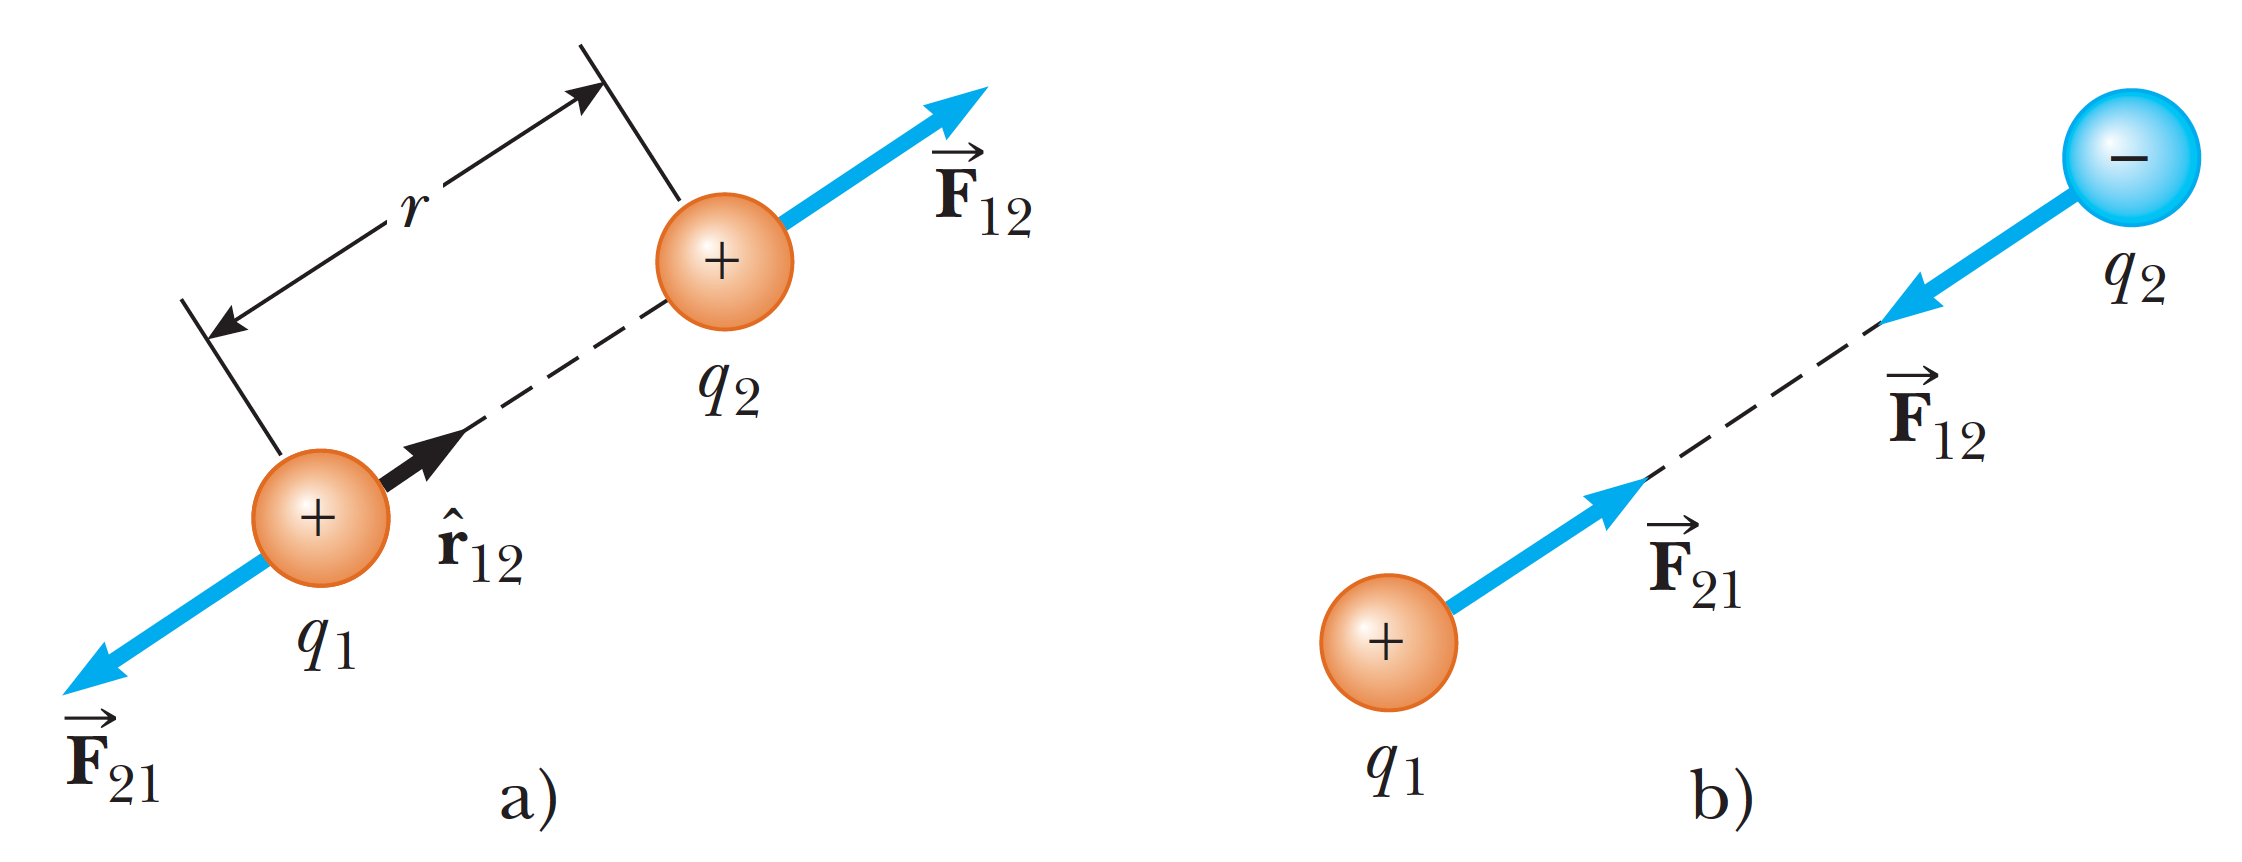
\includegraphics[width=0.5\textwidth]{4/figure_1}
      \caption{Dos cargas puntuales separadas por una distancia $r$ ejercen una fuerza mutua que está determinada por la
      Ley de Coulomb.}
    \end{figure}

    \PN Si $q_{1}$ y $q_{2}$ son del mismo signo, el producto $q_{1} q_{2}$ es positivo. Si $q_{1}$ y $ q_{2}$ son de
    signos opuestos, el producto $q_{1} q_{2}$ es negativo. Estos signos indican la dirección \textit{relativa} de la
    fuerza, pero no la dirección \textit{absoluta}. Un producto negativo indica que se trata de una \textbf{fuerza de
    atracción}, por lo que cada una de las cargas experimenta una fuerza hacia la otra. Un producto positivo indica que
    se trata de una \textbf{fuerza de repulsión} tal que cada carga experimenta una fuerza que la separa de la otra. La
    dirección absoluta de la fuerza sobre una carga depende de la posición de la otra carga.

    \VS
    \PN Cuando hay más de dos cargas presentes, la fuerza resultante de cualquiera de ellas es igual a la suma vectorial
    de las fuerzas ejercidas por las otras cargas individuales. Por ejemplo, si están presentes cuatro cargas, la fuerza
    resultante ejercida por las partículas 2, 3 y 4 sobre la partícula 1 es de
    \begin{equation*}
      \vec{F}_{1} = \vec{F}_{21} + \vec{F}_{31} + \vec{F}_{41}
    \end{equation*}

  \subsection{El campo eléctrico}
    \PN El concepto de campo fue desarrollado por Faraday en relación con las fuerzas eléctricas. En este planteamiento,
    existe un \textbf{campo eléctrico} en la región del espacio que rodea a un objeto con carga: la \textbf{carga
    fuente}. Cuando otro objeto con carga, la \textbf{carga de prueba}, entra en este campo eléctrico, una fuerza
    eléctrica actúa sobre él.

    \VS
    \PN El vector $\vec{E}$ del campo eléctrico en un punto en el espacio se define como la \textbf{fuerza eléctrica}
    $\vec{F}$, que actúa sobre una carga de prueba positiva $q_{0}$ colocada en ese punto, dividida entre la carga de
    prueba
    \begin{equation*}
      \vec{E} \equiv \frac{\vec{F}}{q_{0}}
    \end{equation*}

    \PN El vector $\vec{E}$ está en unidades del SI, newtons por cada coulomb (N/C). Observe que $\vec{E}$ es el campo
    producido por una carga o distribución de carga separada de la carga de prueba; no es el campo producido por la
    propia carga de prueba, además observe que la existencia de un campo eléctrico es una propiedad de su fuente; la
    presencia de una carga de prueba no es necesaria para que el campo exista. La carga de prueba sirve como detector
    del campo eléctrico.

    \VS
    \PN La dirección de $\vec{E}$, es la dirección de la fuerza que experimenta una carga de prueba positiva cuando es
    colocada en el campo; existe un campo eléctrico en un punto si una carga de prueba en dicho punto experimenta una
    fuerza eléctrica.

    \VS
    \PN La fuerza ejercida sobre una partícula con carga $q$ colocada en un campo eléctrico es
    \begin{equation*}
      \vec{F} = q \vec{E}
    \end{equation*}

    \PN Si $q$ es positiva, la fuerza tiene la misma dirección que el campo. Si es negativa, la fuerza y el campo tienen
    direcciones opuestas.

    \VS
    \PN Para determinar la dirección que tiene un campo eléctrico, considere una carga puntual $q$ como carga fuente.
    Esta carga produce un campo eléctrico en todos los puntos del espacio que la rodea. En el punto P, a una distancia
    $r$ de la carga fuente, se coloca una carga de prueba $q_{0}$. Imagine el uso de la carga de prueba para determinar
    la dirección de la fuerza eléctrica y, por lo tanto, la dirección del campo eléctrico. De acuerdo con la ley de
    Coulomb, la fuerza ejercida por $q$ sobre la carga de prueba es
    \begin{equation*}
      \vec{F} = k \ \frac{q q_{0}}{r^{2}} \ \hat{r}
    \end{equation*}

    \PN dónde $\hat{r}$ es un vector unitario con dirección de $q$ hacia $q_{0}$.

    \begin{figure}[H]
    \centering
      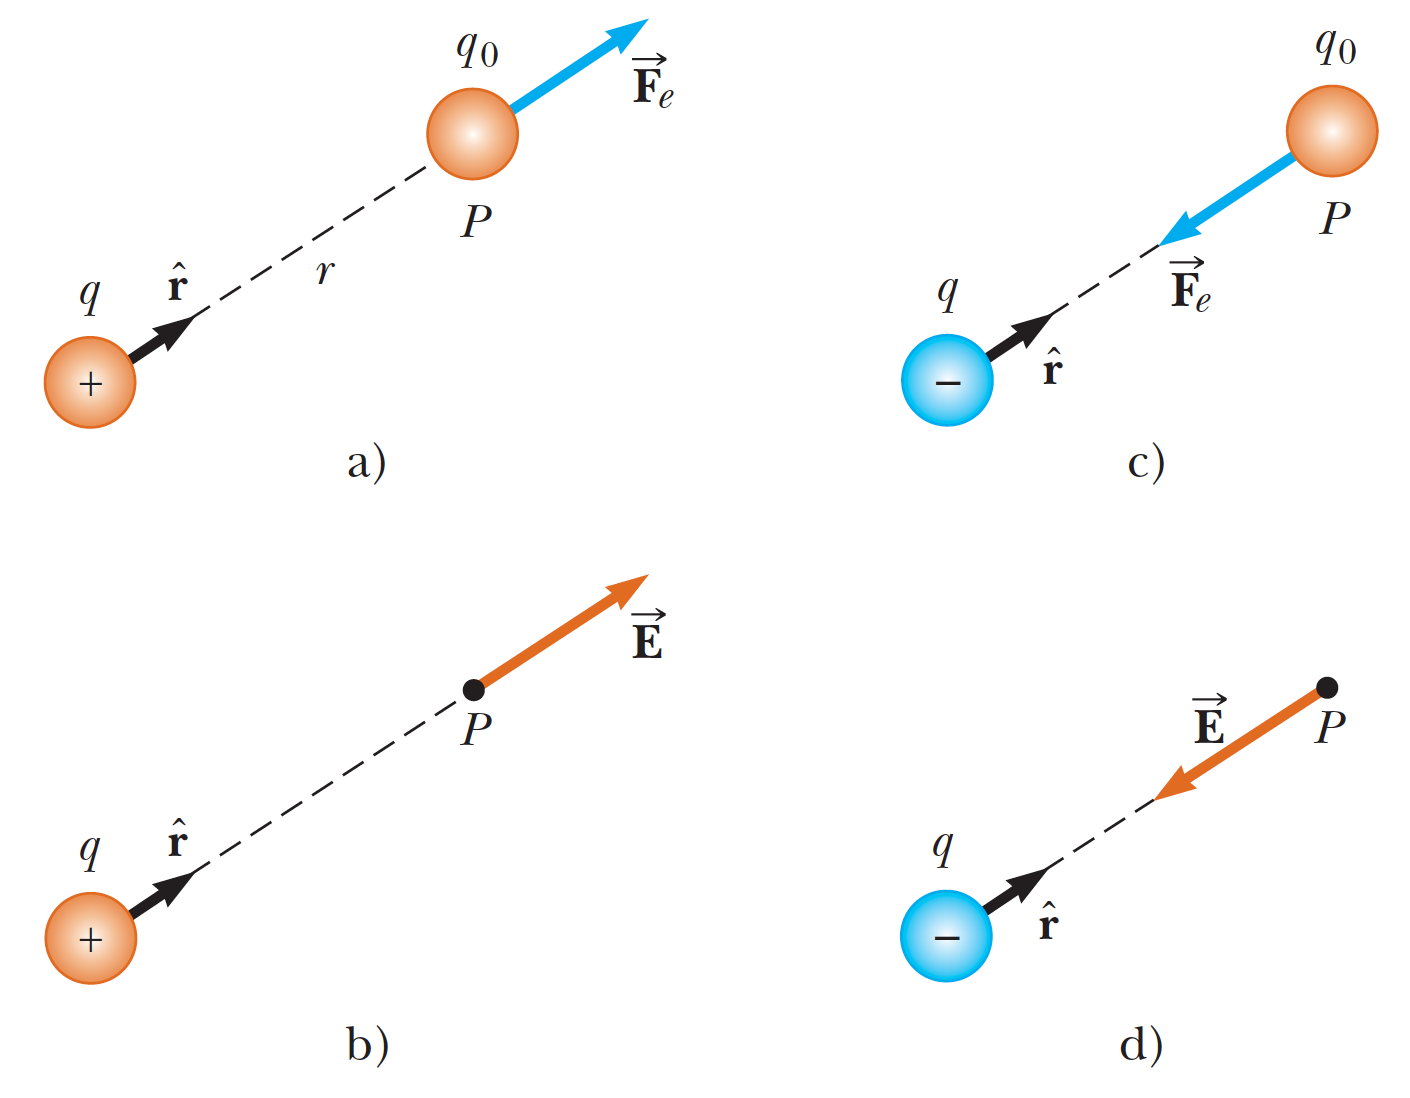
\includegraphics[width=0.45\textwidth]{4/figure_2}
      \caption{Una carga de prueba $q_{0}$ en el punto P está a una distancia $r$ de la carga puntual $q$.}
    \end{figure}

    \PN Ya que el campo eléctrico en P, que es la posición de la carga de prueba, queda definido por $\vec{E} = \vec{F}
    / q_{0}$, el campo eléctrico en P establecido por $q$ es
    \begin{equation*}
      \vec{E} = k \ \frac{q}{r^{2}} \ \hat{r}
    \end{equation*}

    \PN El campo eléctrico en el punto P debido a un grupo de cargas fuente se expresa como la suma vectorial
    \begin{equation*}
      \vec{E} = k \ \sum_{i} \frac{q_{i}}{r_{i}^{2}} \ \hat{r}_{i}
    \end{equation*}

    \PN donde $r_{i}$ es la distancia desde la i-ésima carga fuente $q_{i}$ hasta el punto P y $\hat{r}^{i}$ es un
    vector unitario dirigido de $q_{i}$ hacia P.

    \VS
    \PN \underline{Dipolo eléctrico:} se define como una carga positiva $q$ y una carga negativa $q$ separadas por una
    distancia $2d$. El dipolo eléctrico es un buen modelo de muchas moléculas. Los átomos y moléculas neutros se
    comportan como dipolos cuando se colocan en un campo eléctrico externo.

  \subsection{Campo eléctrico de una distribución de carga continua}
    \PN Con mucha frecuencia, en un grupo de cargas, la distancia existente entre ellas es mucho más reducida que la
    distancia entre el grupo y el punto donde se desea calcular el campo eléctrico. En esta situación, el sistema de
    cargas se modela como si fuera continuo. Es decir, el sistema de cargas espaciadas en forma compacta es equivalente
    a una carga total que es distribuida de forma continua a lo largo de alguna línea, sobre alguna superficie, o por
    todo el volumen.

    \VS El campo eléctrico en P debido a un elemento de carga con una carga $\Delta q$ es
    \begin{equation*}
      \Delta \vec{E} = k \ \frac{\Delta q}{r^{2}} \ \hat{r}
    \end{equation*}

    \PN donde $r$ es la distancia desde el elemento de carga hasta el punto P y $\hat{r}$ es el vector unitario
    dirigido desde el elemento de carga hasta P. El campo eléctrico total en P debido a todos los elementos en la
    distribución de carga es aproximadamente
    \begin{equation*}
      \vec{E} \approx k \ \sum_{i} \frac{\Delta q_{i}}{r_{i}^{2}} \ \hat{r}_{i}
    \end{equation*}

    \PN donde el índice $i$ se refiere al i-ésimo elemento de orden $i$ en la distribución. Ya que la distribución de
    carga ha sido modelada como continua, el campo total en P en el límite $\Delta q_{i} \rightarrow 0$ es
    \begin{equation*}
      \vec{E} = k \ \lim_{\Delta q_{i} \rightarrow 0} \ \sum_{i} \frac{\Delta q_{i}}{r_{i}^{2}} \ \hat{r}_{i} = k \ \int
      \ \frac{dq}{r^{2}} \ \hat{r}
    \end{equation*}

    \PN donde la integración es sobre toda la distribución de carga. La integración de la ecuación anterior es una
    operación vectorial y debe ser tratada en forma apropiada.

    \VS
    \PN Este tipo de cálculo se ilustra con varios ejemplos en los que la carga está distribuida a lo largo de una
    línea, sobre una superficie, o en todo un volumen. Cuando realice estos cálculos es conveniente que use el concepto
    de densidad de carga junto con las siguientes observaciones:
    \begin{itemize}
      \item Si una carga Q tiene una distribución uniforme en un volumen V, la \textbf{densidad de carga volumétrica}
      $\rho$ se define como
      \begin{equation*}
        \rho \equiv \frac{\text{Q}}{\text{V}}
      \end{equation*}

      \PN donde $rho$ está en C/$m^{3}$.

      \item Si una carga Q tiene una distribución uniforme sobre una superficie de área A, la \textbf{densidad de carga
      superficial} $\sigma$ se define como
      \begin{equation*}
        \sigma \equiv \frac{\text{Q}}{\text{A}}
      \end{equation*}

      \PN donde $sigma$ está en C/$m^{2}$.

      \item Si una carga Q tiene una distribución uniforme a lo largo de una línea de longitud $l$, la \textbf{densidad
      de carga lineal} $\lambda$ se define como
      \begin{equation*}
        \lambda \equiv \frac{\text{Q}}{l}
      \end{equation*}

      \PN donde $lambda$ está en C/$m$.

      \item Si la carga no tiene distribución uniforme en un volumen, superficie o línea, las cantidades de cargas $dq$
      en un elemento pequeño de volumen, superficie o longitud son
      \begin{equation*}
        dq = \rho \ d \text{V} \qquad dq = \sigma \ d \text{A} \qquad dq = \lambda \ dl
      \end{equation*}
    \end{itemize}

    \subsection{Líneas de campo eléctrico}
      \PN Una forma conveniente de visualizar los patrones de los campos eléctricos es el trazo de líneas conocidas
      como \textbf{líneas de campo eléctrico}, establecidas por primera vez por Faraday, las cuales relacionan el campo
      eléctrico con una región del espacio.

      \begin{figure}[H]
        \centering
        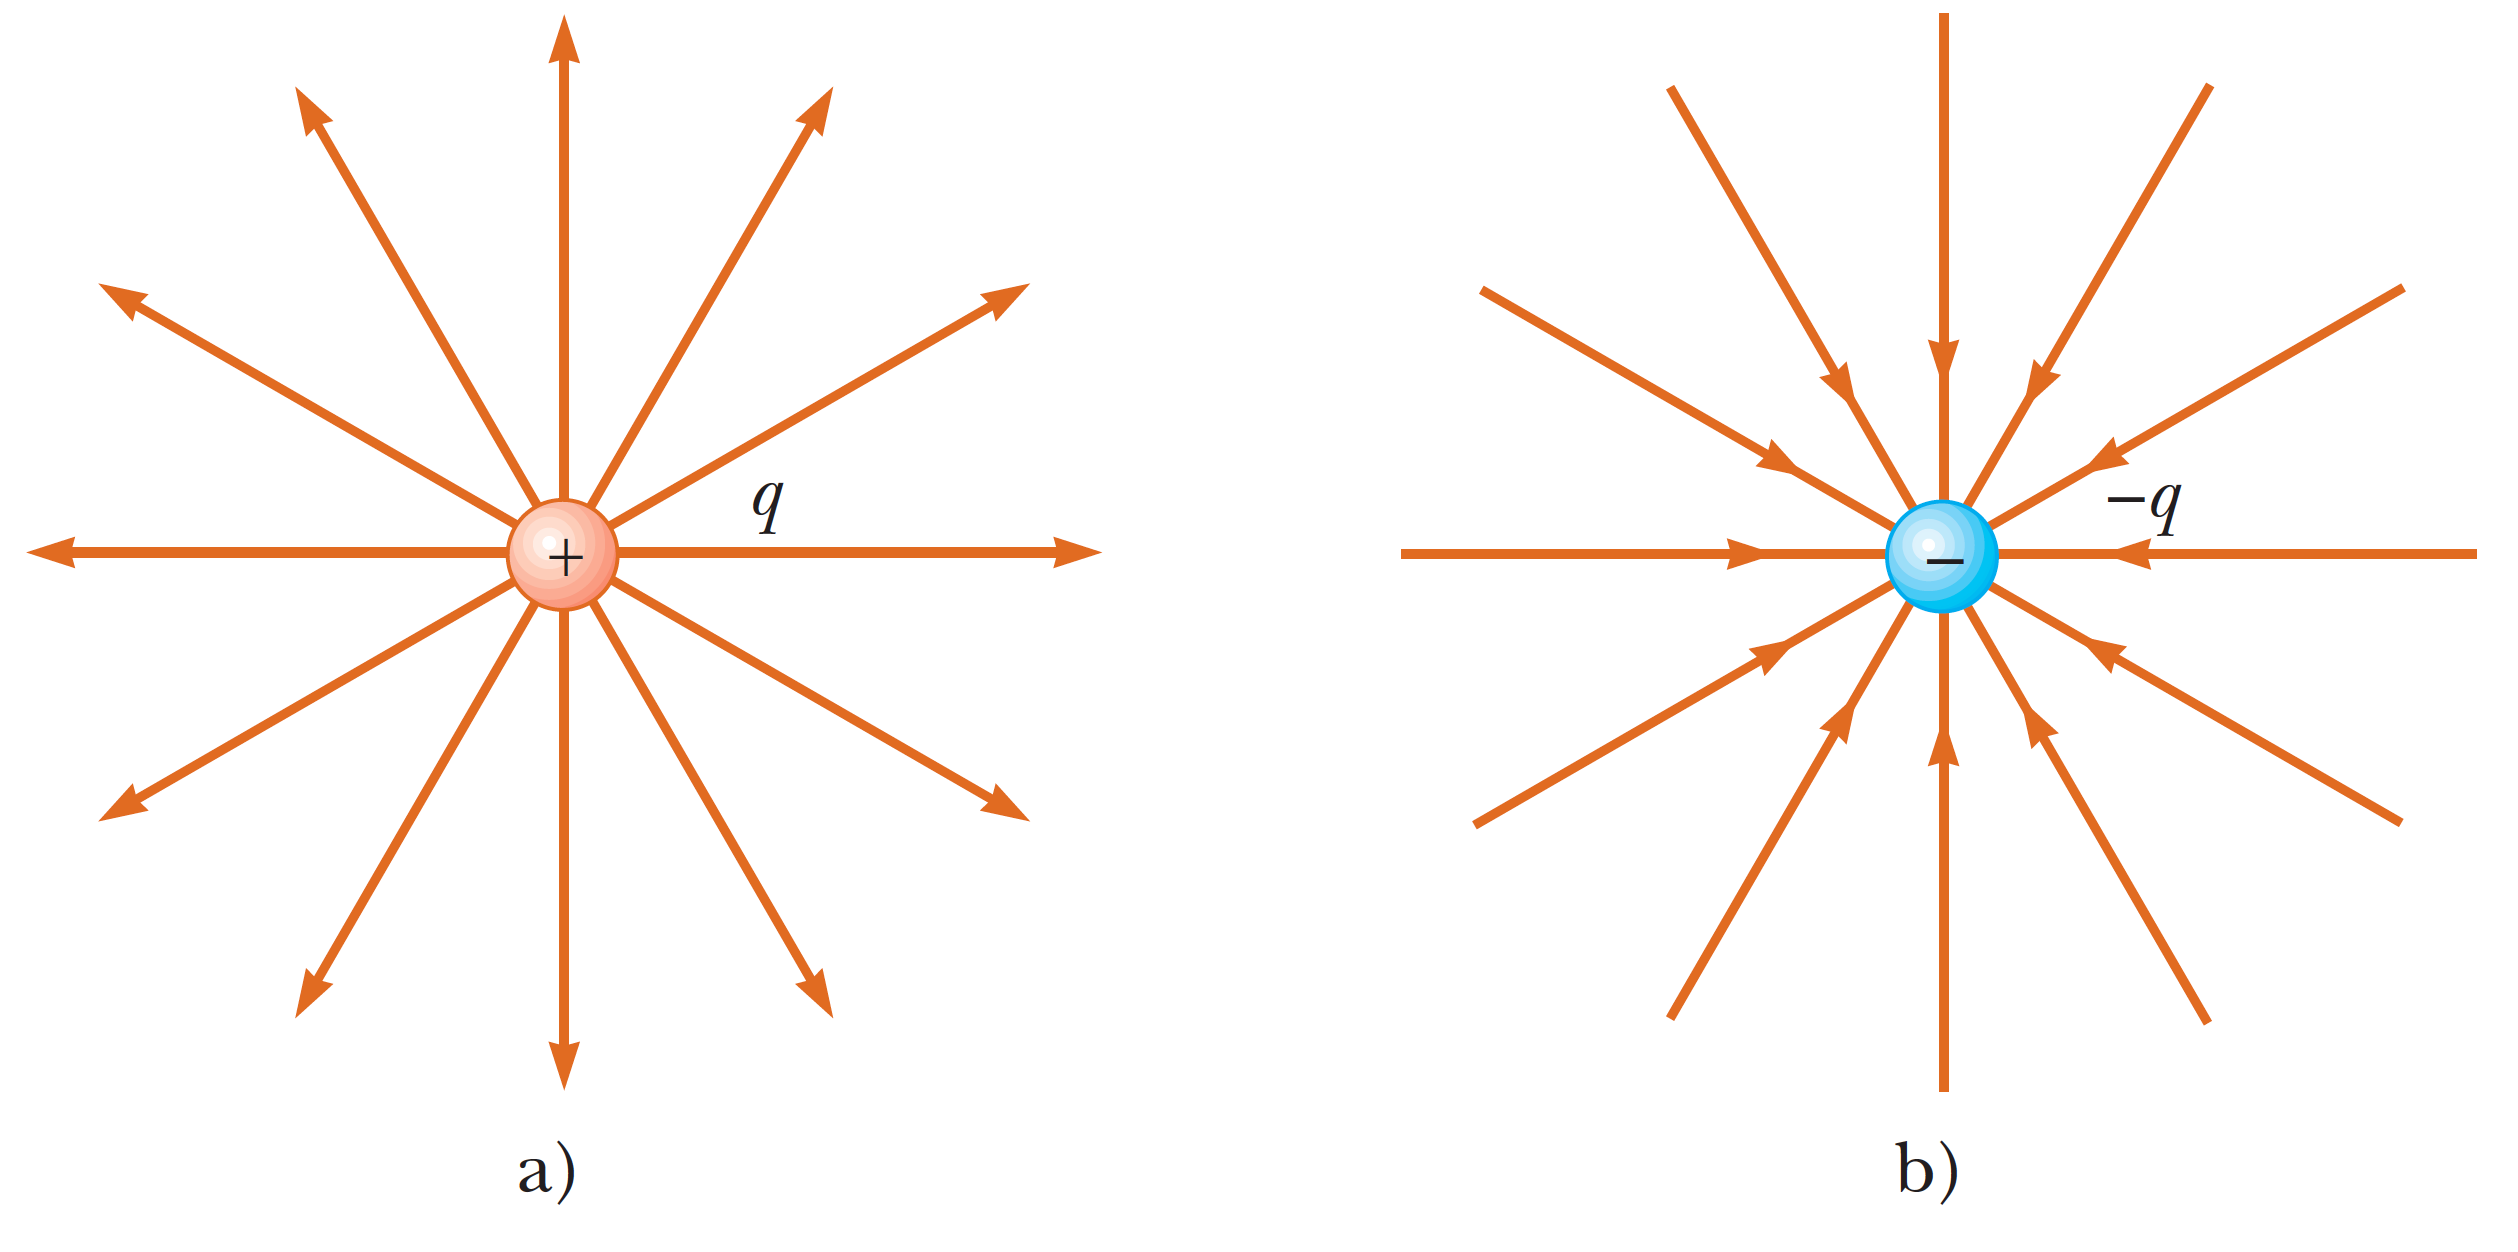
\includegraphics[width=0.6\textwidth]{4/figure_3}
        \caption{Líneas de campo eléctrico para una carga puntual.}

        \begin{multicols}{2}
          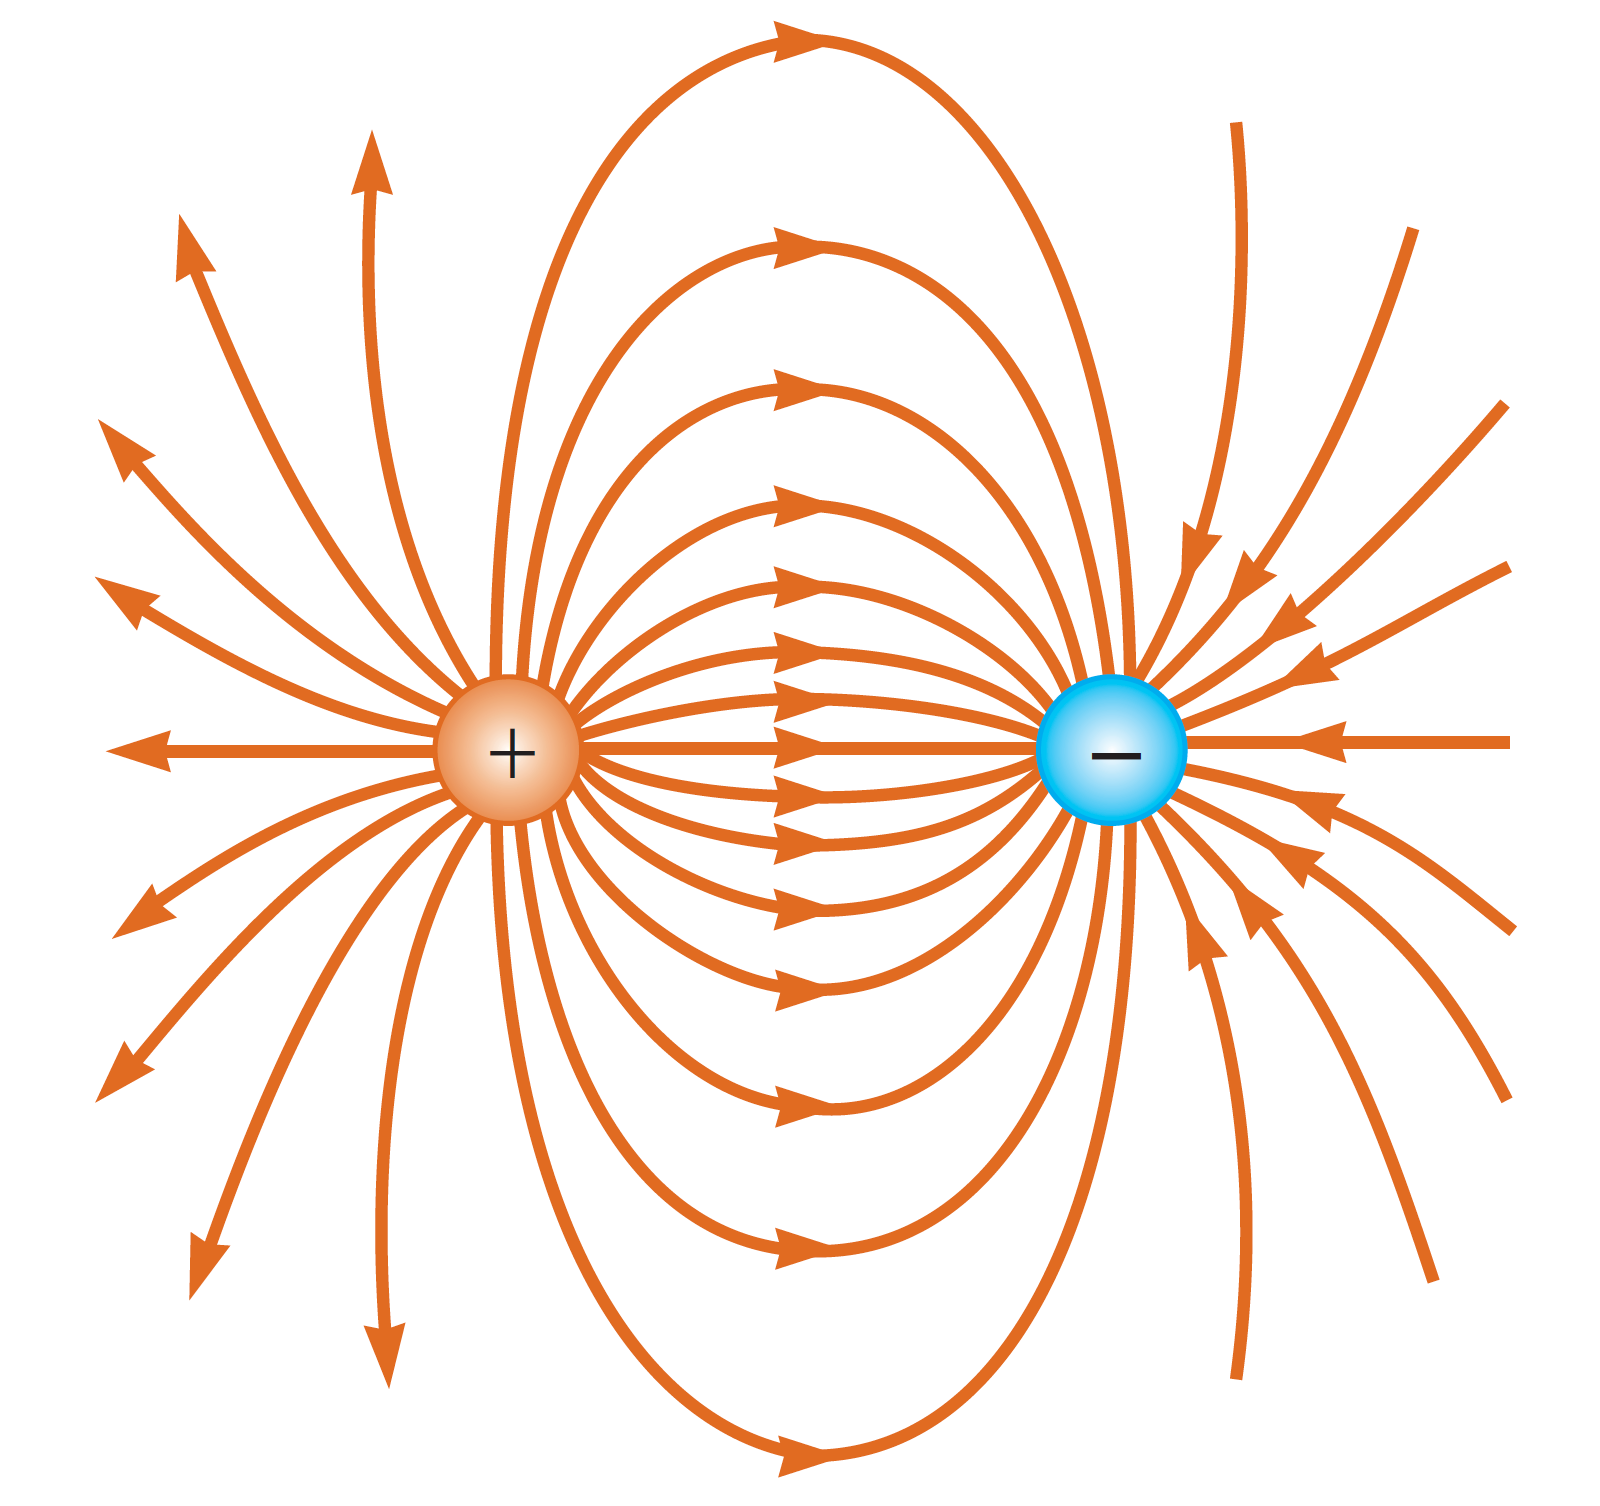
\includegraphics[width=0.3\textwidth]{4/figure_4}\par
          \caption{Líneas de campo eléctrico para dos cargas puntuales de igual magnitud y de signo opuesto.}
          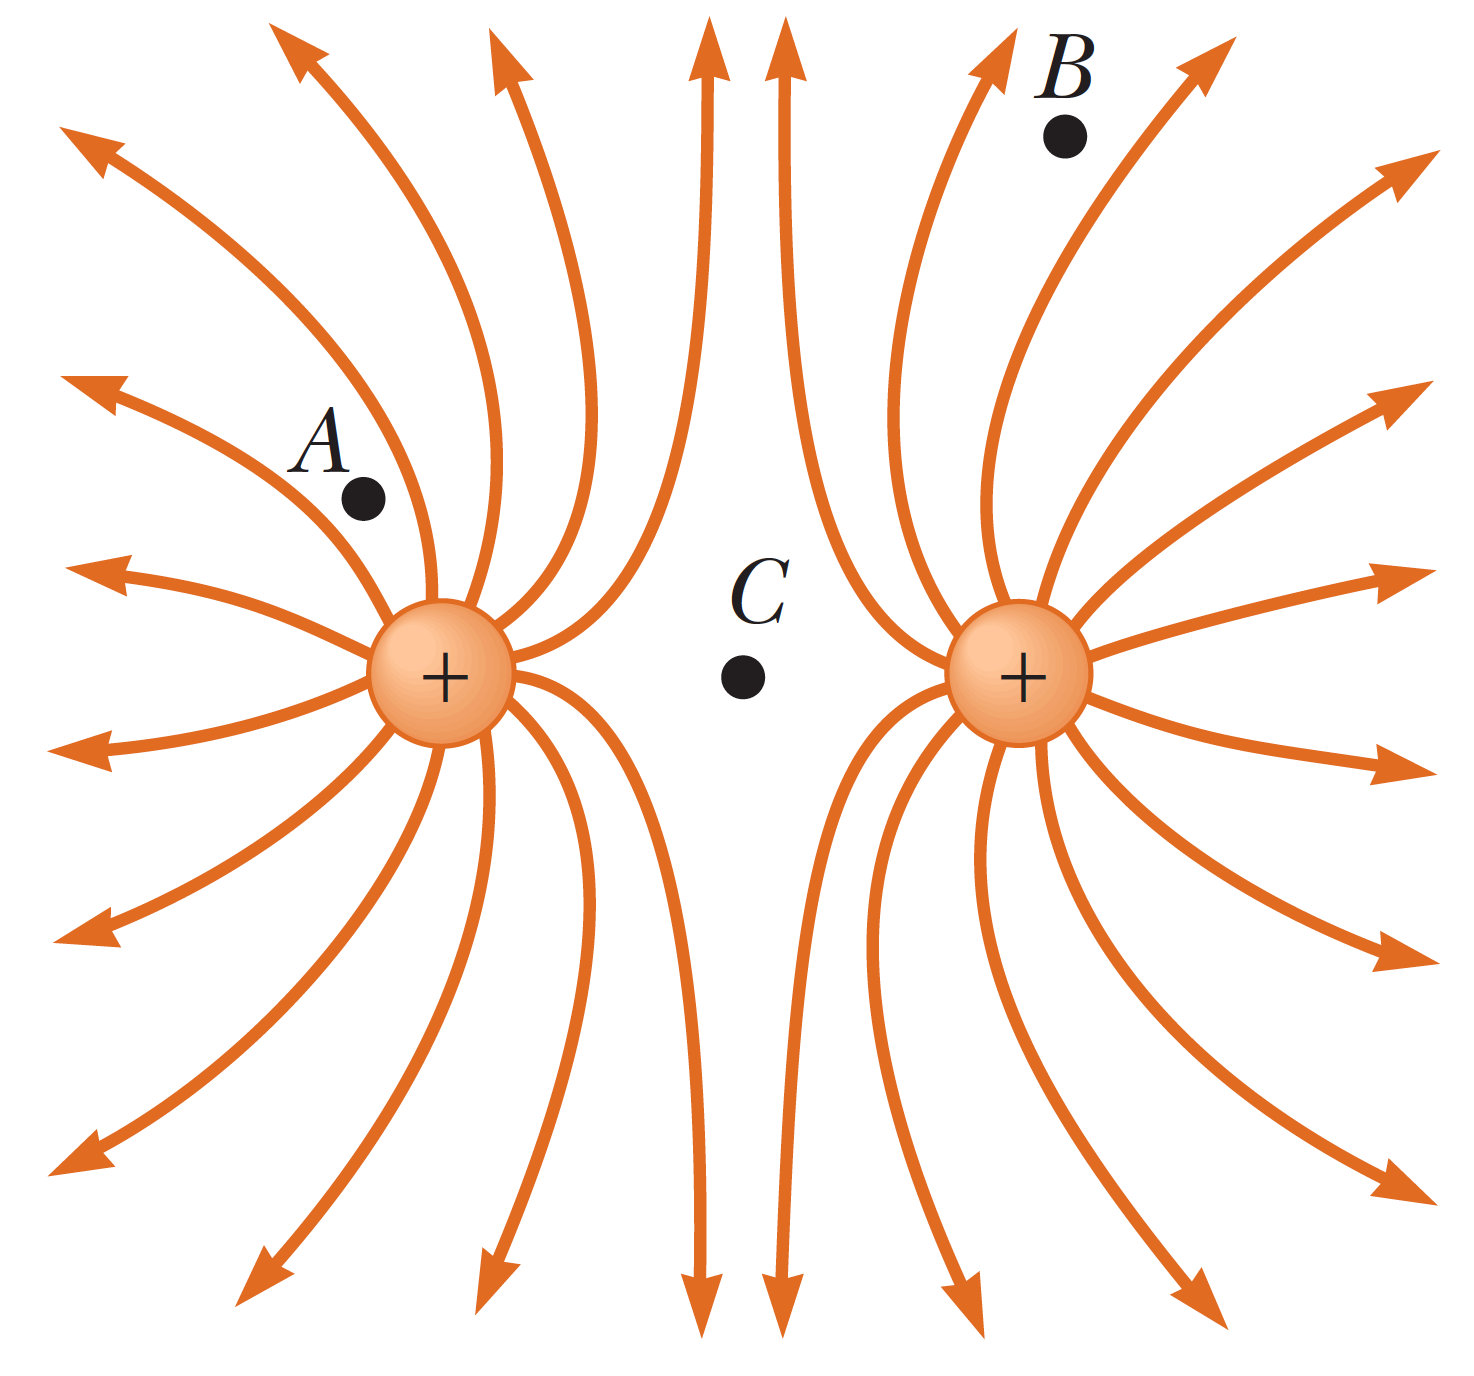
\includegraphics[width=0.3\textwidth]{4/figure_5}\par
          \caption{Líneas de campo eléctrico para dos cargas puntuales positivas.}
        \end{multicols}
      \end{figure}

		\section{Ley de Gauss}
  \subsection{Flujo eléctrico}
    \PN El total de líneas que penetran en la superficie es proporcional al producto $EA$. A este producto de la
    magnitud del campo eléctrico $E$ y al área superficial $A$, perpendicular al campo, se le conoce como \textbf{flujo
    eléctrico} $\Phi$.
    \begin{equation*}
      \Phi = EA \cos(\theta)
    \end{equation*}

    \PN Con base en las unidades del SI correspondientes a $E$ y $A$, $\Phi$ se expresa en (N $m^{2} /$ C). El flujo
    eléctrico es proporcional al número de las líneas de campo eléctrico que penetran en una superficie.

    \PN Considere una superficie dividida en un gran número de elementos pequeños, cada uno de área $\Delta A$. Es
    conveniente definir un vector $\Delta \vec{A}_{i}$ cuya magnitud representa el área del elemento i-ésimo sobre la
    superficie y cuya dirección está definida como perpendicular al elemento de superficie. El campo eléctrico $\vec{E}$
    en la ubicación de este elemento forma un ángulo $u_{i}$ con el vector $\Delta \vec{A}_{i}$. El flujo eléctrico
    $\Delta \Phi$ a través de este elemento es
    \begin{equation*}
      \Delta \Phi = E_{i} \Delta A_{i} \cos(\theta_{i}) = \vec{E} \Delta \vec{A}_{i}
    \end{equation*}

    \PN Al sumar las contribuciones de todos los elementos, obtiene el flujo total a través de la superficie.
    \begin{equation*}
      \Phi \approx \sum \vec{E}_{i} \Delta \vec{A}_{i}
    \end{equation*}

    \PN Si supone que el área de cada elemento se acerca a cero, en tal caso el número de elementos se acercaría al
    infinito y la suma se reemplaza por una integral. Debido a eso, la definición general del flujo eléctrico es
    \begin{equation*}
      \Phi = \oint \vec{E} \ d\vec{A}
    \end{equation*}

    \PN El flujo neto a través de la superficie es proporcional al número neto de líneas que salen de la superficie,
    donde número neto significa la cantidad de líneas que salen de la superficie menos la cantidad de líneas que entran.

    \subsection{Ley de Gauss}
      \PN La Ley de Gauss se define como la correspondencia de tipo general entre el flujo eléctrico neto a través de
      una superficie cerrada y la carga encerrada en la superficie.

      \PN Suponga de nuevo una carga puntual positiva $q$ ubicada en el centro de una esfera de radio $r$. Se sabe que
      la magnitud del campo eléctrico en todos los puntos de la superficie de la esfera es $E = k q/r^{2}$. Las líneas
      de campo están dirigidas radialmente hacia afuera y por tanto son perpendiculares a la superficie en todos sus
      puntos. Es decir, en cada punto de la superficie, $\vec{E}$ es paralelo al vector $\Delta \vec{A}$ que representa
      un elemento de área local $\Delta A_{i}$ que rodea al punto en la superficie. Por lo tanto
      \begin{equation*}
        \vec{E} \ \Delta \vec{A}_{i} = E \ \Delta A
      \end{equation*}

      \PN y el flujo neto a través de la superficie gaussiana es igual a
      \begin{equation*}
        \Phi = \oint \vec{E} d\vec{A} = \oint E dA = E \oint dA
      \end{equation*}

      \PN donde se ha retirado $E$ afuera de la integral ya que, por simetría, $E$ es constante en la superficie y se
      conoce por $E = k q/r^{2}$. Además, en vista de que la superficie es esférica, $\oint dA = A = 4 \pi r^{2}$. Por
      lo tanto, el flujo neto a través de la superficie gaussiana es
      \begin{equation*}
        \Phi = k \frac{q}{r^{2}} (4 \pi r^{2}) = 4 \pi kq
      \end{equation*}

      \PN Dado que $k = 1/4 \pi \varepsilon_{0}$, escribimos
      \begin{equation*}
        \Phi = \frac{q}{\varepsilon_{0}}
      \end{equation*}

      \PN \textbf{\underline{Observaciones}}
      \begin{itemize}
        \item el flujo neto a través de cualquier superficie cerrada que rodea a una carga puntual $q$ tiene un valor de
        $q/e_{0}$ y es independiente de la forma de la superficie.
        \item el flujo eléctrico neto a través de una superficie cerrada que no rodea a ninguna carga es igual a cero.
      \end{itemize}

    \subsection{Conductores en equilibrio estático}
      \PN Un buen conductor eléctrico contiene cargas (electrones) que no se encuentran unidas a ningún átomo y debido a
      eso tienen la libertad de moverse en el interior del material. Cuando dentro de un conductor no existe ningún
      movimiento neto de carga, el conductor está en \textbf{equilibrio electrostático}. Un conductor en equilibrio
      electrostático tiene las siguientes propiedades:
      \begin{itemize}
        \item En el interior del conductor el campo eléctrico es cero, si el conductor es sólido o hueco.
        \item Si un conductor aislado tiene carga, ésta reside en su superficie.
        \item El campo eléctrico justo fuera de un conductor con carga es perpendicular a la superficie del conductor y
        tiene una magnitud $s/e_{0}$, donde $s$ es la densidad de carga superficial en ese punto.
        \item En un conductor de forma irregular, la densidad de carga superficial es máxima en aquellos puntos donde el
        radio de curvatura de la superficie es el menor.
      \end{itemize}

		\section{Potencial eléctrico}
  \PN Cuando se coloca una carga de prueba $q_{0}$ en un campo eléctrico $\vec{E}$ producido por alguna distribución de
  carga fuente, la fuerza eléctrica que actúa sobre ella es $q_{0} \vec{E}$. La fuerza $q_{0}\vec{E}$ es conservativa,
  ya que la fuerza entre cargas descrita por la ley de Coulomb es conservativa. Cuando se traslada la carga de prueba
  por algún agente externo en el campo, el trabajo consumido por el campo en la carga es igual al trabajo invertido por
  el agente externo que origina el desplazamiento, pero con signo negativo.

  \VS
  \PN Al analizar los campos eléctricos y magnéticos, es común utilizar la notación $d\vec{s}$ para representar un
  vector de desplazamiento infinitesimal que tiene una orientación tangente a una trayectoria a través del espacio. Esta
  trayectoria puede ser recta o curva, y la integral calculada a lo largo de esta trayectoria se conoce como integral de
  la trayectoria, o bien, integral de línea.

  \VS
  \PN Para un desplazamiento infinitesimal $d\vec{s}$ de una carga puntual $q_{0}$ inmersa en un campo eléctrico, el
  trabajo realizado por un campo eléctrico sobre la misma es $\vec{F} d\vec{s} = q_{0} \vec{E} ds$. Conforme el campo
  consume esta cantidad de trabajo, la energía potencial del sistema carga-campo cambia en una cantidad $dU = -q_{0}
  \vec{E} d\vec{s}$. Para un desplazamiento finito de la carga desde el punto A al punto B, el cambio en energía
  potencial del sistema $\Delta U = U_{B} - U_{A}$ es
  \begin{equation*}
    \Delta U = -q_{0} \int_{A}^{B} \vec{E} \ d\vec{s}
  \end{equation*}

  \PN La integración se lleva a cabo a lo largo de la trayectoria que $q_{0}$ sigue al pasar de A a B. Porque la fuerza
  $q_{0}\vec{E}$ es conservativa, la integral de línea no depende de la trayectoria de A a B.

  \VS
  \PN Al dividir la energía potencial entre la carga de prueba se obtiene una cantidad física que depende sólo de la
  distribución de carga fuente y tiene un valor en cada uno de los puntos de un campo eléctrico. Esta cantidad se conoce
  como \textbf{potencial eléctrico} ($V$):
  \begin{equation*}
    V = \frac{U}{q_{0}}
  \end{equation*}

  \PN Si la carga de prueba es desplazada entre las posiciones A y B en un campo eléctrico, el sistema carga-campo
  experimenta un cambio en su energía potencial. La \textbf{diferencia de potencial} $\Delta V = V_{B} - V_{A}$ entre
  los puntos A y B de un campo eléctrico se define como el cambio en energía potencial en el sistema al mover una carga
  de prueba $q_{0}$ entre los puntos, dividido entre la carga de prueba:
  \begin{equation*}
    \Delta V \equiv \frac{\Delta U}{q_{0}} = - \int_{A}^{B} \vec{E} \ d\vec{s}
  \end{equation*}

  \PN Si un agente externo traslada una carga de prueba de A a B sin modificar la energía cinética de ésta, el agente
  realiza un trabajo que modifica la energía potencial del sistema: $W = \Delta U$. Imagine una carga $q$ arbitraria
  localizada en un campo eléctrico. El trabajo consumido por un agente externo al desplazar una carga $q$ a través de un
  campo eléctrico con una velocidad constante es
  \begin{equation*}
    W = q \Delta V
  \end{equation*}

  \PN Ya que el potencial eléctrico es una medida de la energía potencial por unidad de carga, la unidad del SI, tanto
  del potencial eléctrico como de la diferencia de potencial, es joules por cada coulomb, que se define como un
  \textbf{volt} (V):
  \begin{equation*}
    1 \ \text{V} \equiv 1 \ \frac{\text{J}}{\text{C}}
  \end{equation*}

  \PN Como conclusión, el campo eléctrico es una medida de la relación de cambio en función de la posición del potencial
  eléctrico.

		\section{Capacitancia y materiales dieléctricos}
  \subsection{Definición de capacitancia}
    \PN La combinación de dos conductores se conoce como \textbf{capacitor}. Los conductores son las placas. Si los
    conductores llevan carga de igual magnitud y signo opuesto existe una diferencia de potencial $\Delta V$ entre
    ellos.

    \VS
    \PN La cantidad de carga Q en un capacitor es linealmente proporcional a la diferencia de potencial entre los
    conductores; es decir, $Q \propto V$. La constante de proporcionalidad depende de la forma y separación de los
    conductores. Esta relación se escribe como $Q = C \Delta V$ si define la capacitancia de la siguiente manera:

    \VS
    \PN \textbf{Definición:} La \textbf{capacitancia} $C$ de un capacitor se define como la relación de la magnitud de
    la carga en cualquiera de los conductores a la magnitud de la diferencia de potencial entre dichos conductores:
    \begin{equation*}
      C \equiv \frac{Q}{\Delta V}
    \end{equation*}

    \PN La capacitancia siempre es una cantidad positiva. Además, la carga $Q$ y la diferencia de potencial $\Delta V$
    siempre se expresan como cantidades positivas.

    \VS
    \PN En unidades del SI la capacitancia se expresa en coulombs por cada volt. La unidad del SI para capacitancia es
    el \textit{farad} (F).
    \begin{equation*}
      1 \ \text{F} = 1 \ \frac{\text{C}}{\text{V}}
    \end{equation*}

    \PN Piense en un capacitor formado por un par de placas paralelas, cada placa está conectada a una de las terminales
    de una batería, que actúa como fuente de diferencia de potencial. Si al inicio el capacitor no está cargado, la
    batería establece una campo eléctrico en los alambres de conexión cuando se cierra el circuito. La diferencia de
    potencial entre las capas del capacitor es la misma que existe entre las terminales de la batería.

  \subsection{Cálculo de la capacitancia}
    \PN Es posible deducir una expresión para la capacitancia producida por un par de conductores de cargas opuestas con
    una carga de magnitud $Q$, de la siguiente manera: primero calcule la diferencia de potencial. A continuación
    utilice la expresión $C = Q / \Delta V$ a fin de evaluar la capacitancia.
    \PN Sin embargo, la situación más común es que de dos conductores, solo un conductor también tenga capacitancia. Por
    ejemplo, imagine un conductor esférico con carga. Las líneas del campo eléctrico alrededor de este conductor son
    exactamente las mismas que si se tratara de una cubierta conductora, esférica de radio infinito, concéntrico con la
    esfera, y con una carga de la misma magnitud pero de signo opuesto. Por lo tanto, identifique esta cubierta
    imaginaria como el segundo conductor de un capacitor de dos conductores. El potencial eléctrico de una esfera de
    radio r es simplemente $k Q/a$, y si $V = 0$ en el caso de la cubierta infinitamente grande, tiene
    \begin{equation*}
      C = \frac{Q}{\Delta V} = \frac{Q}{k Q/a} = \frac{r}{k} = 4 \pi \epsilon_{0} r
    \end{equation*}

    \PN Esta expresión muestra que la capacitancia de una esfera con carga y aislada es proporcional a su radio y es
    independiente tanto de la carga de la esfera como de la diferencia de potencial.

    \PN La capacitancia de un par de conductores se ilustra mediante tres geometrías comunes, sobre todo, placas
    paralelas, cilindros concéntricos y esferas concéntricas. En estos ejemplos, suponga que los conductores cargados
    están separados por un espacio vacío.

    \subsubsection{Capacitor de placas paralelas}
      \PN Dos placas metálicas paralelas de igual área $A$ están separadas por una distancia $d$. Una placa tiene una
      carga $+Q$ y la otra tiene una carga $–Q$. La densidad de carga superficial en cada placa es $ \sigma = Q/A$. El
      valor del campo eléctrico entre las placas es
      \begin{equation*}
        E = \frac{\sigma}{\epsilon_{0}} = \frac{Q}{\epsilon_{0}A}
      \end{equation*}

      \PN Ya que el campo entre las placas es uniforme, la magnitud de la diferencia de potencial entre las placas es
      igual a Ed, por lo tanto
      \begin{equation*}
        \Delta V = Ed = \frac{Qd}{\epsilon_{0}A}
      \end{equation*}

      \PN Luego, la capacitancia es
      \begin{equation*}
        C = \frac{Q}{\Delta V} = \frac{Q}{Qd/\epsilon_{0}A} = \frac{\epsilon_{0}A}{d}
      \end{equation*}

      \PN Es decir, la capacitancia de un capacitor de placas paralelas es proporcional al área de sus placas e
      inversamente proporcional a la separación de las placas.

  \subsection{Combinaciones de capacitores}
    \PN En los circuitos eléctricos con frecuencia se combinan dos o más capacitores. Es posible calcular la
    capacitancia equivalente de ciertas combinaciones, en donde supondrá que los capacitores a combinar están
    inicialmente descargados.

    \subsubsection{Combinación en paralelo}
      \begin{figure}[H]
      \centering
        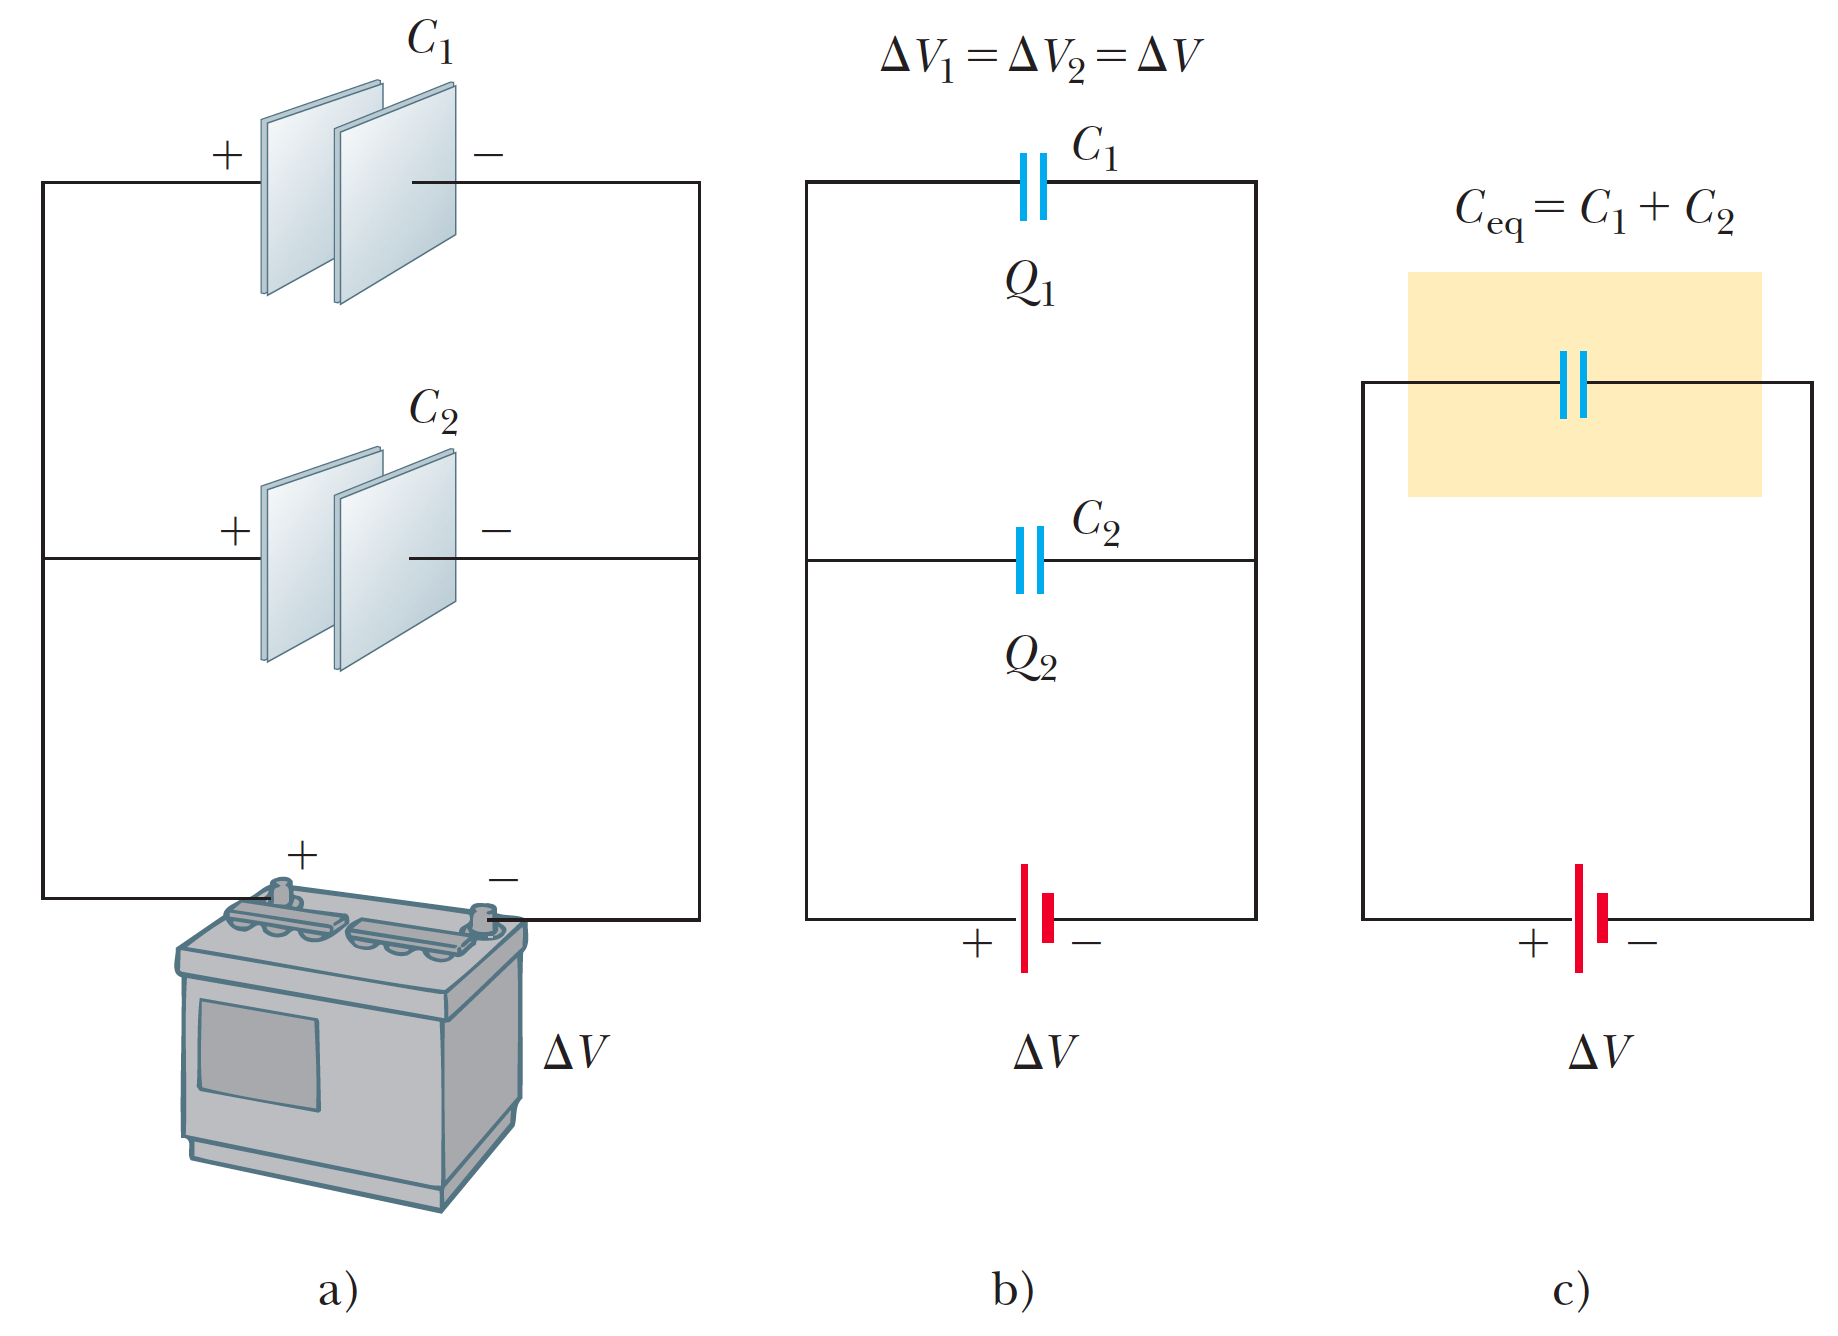
\includegraphics[width=0.55\textwidth]{4/figure_6}
        \caption{a) Una combinación en paralelo de dos capacitores en un circuito eléctrico en el cual la diferencia de
        potencial entre las terminales de la batería, es igual a V. b) Diagrama de circuito para esta combinación en
        paralelo. c) La capacitancia equivalente.}
      \end{figure}

      \PN Las diferencias de potencial individuales a través de capacitores conectados en paralelo son las mismas e
      iguales a la diferencia de potencial aplicada a través de la combinación. Es decir,
      \begin{equation*}
        \Delta V = \Delta V_{1} = \Delta V_{2}
      \end{equation*}

      \PN donde $\Delta V$ es el voltaje de terminal de la batería.

      \VS
      \PN Después de que la batería se une al circuito, los capacitores rápidamente alcanzan su carga máxima. Sean las
      cargas máximas en los dos capacitores $Q_{1}$ y $Q_{2}$. La carga total $Q_{tot}$ almacenada por los dos
      capacitores es
      \begin{equation*}
        Q_{tot} = Q_{1} + A_{2}
      \end{equation*}

      \PN Es decir, la carga total en capacitores conectados en paralelo es la suma de las cargas en los capacitores
      individuales.

      \VS
      \PN Suponga que quiere sustituir estos dos capacitores por un capacitor equivalente que tenga una capacitancia
      $C_{eq}$. El efecto que este capacitor equivalente tiene sobre el circuito debe ser exactamente el mismo que el
      efecto de la combinación de los dos capacitores individuales. Es decir: el capacitor equivalente debe almacenar
      carga $Q_{tot}$ cuando se conecte a la batería. El voltaje a través del capacitor equivalente es $\Delta V$ porque
      el capacitor equivalente se conecta directamente a través de las terminales de la batería. Por lo tanto, para el
      capacitor equivalente,
      \begin{equation*}
        Q_{tot} = C_{eq} \ \Delta V
      \end{equation*}

      \PN Luego
      \begin{eqnarray*}
        C_{eq} \ \Delta V = C_{1} \ \Delta V_{1} = C_{2} \ \Delta V_{2} \\
        C_{eq} = C_{1} + C_{2} \ \text{(combinaciones en paralelo)}
      \end{eqnarray*}

      \PN donde se cancelan los voltajes porque todos son iguales. Si este tratamiento se extiende a tres o más
      capacitores conectados en paralelo, se encuentra que la capacitancia equivalente
      \begin{equation*}
        C_{eq} = C_{1} + C_{2} + \dotsc \ \text{(combinaciones en paralelo)}
      \end{equation*}

    \subsubsection{Combinación en serie}
      \begin{figure}[H]
      \centering
        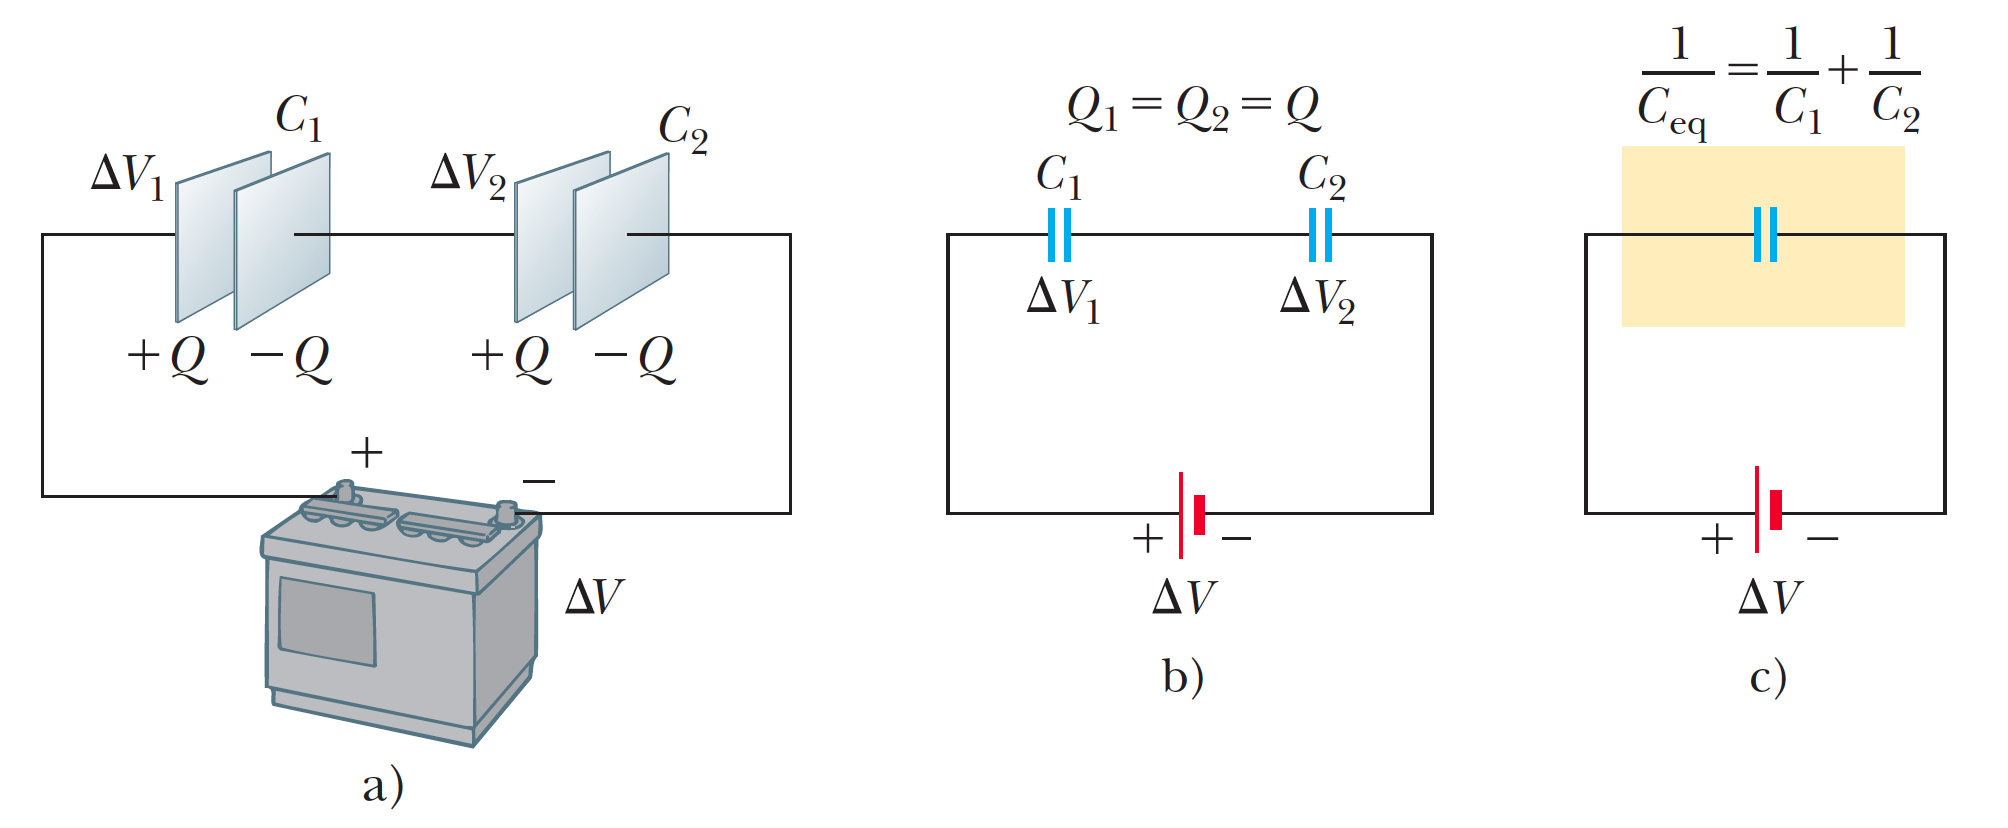
\includegraphics[width=0.7\textwidth]{4/figure_7}
        \caption{a) Combinación en serie de dos capacitores. Las cargas en ambos capacitores son iguales. b) Diagrama
        del circuito para la combinación en serie. c) La capacitancia equivalente.}
      \end{figure}

      \PN Las cargas de los capacitores conectados en serie son iguales.
      \begin{equation*}
        Q = Q_{1} = Q_{2}
      \end{equation*}

      \PN donde $Q$ es la carga que se movió entre un alambre y la placa exterior conectada de uno de los capacitores.

      \PN El voltaje total $V_{tot}$ a través de la combinación se divide entre los dos capacitores:
      \begin{equation*}
        \Delta V_{tot} = \Delta V_{1} + \Delta V_{2}
      \end{equation*}

      \PN donde $V_{1}$ y $V_{2}$ son las diferencias de potencial presentes en los capacitores $C_{1}$ y $C_{2}$,
      respectivamente. En general, la diferencia de potencial total aplicada a cualquier cantidad de capacitores
      conectados en serie es la suma de las diferencias de potencial presentes entre cada uno de los capacitores
      individuales.

      \VS
      \PN Suponga que el simple capacitor individual equivalente ejerce un efecto idéntico sobre el circuito que la
      combinación en serie cuando está conectado a la batería. Una vez que está totalmente cargado, el capacitor
      equivalente deberá tener una carga igual a $-Q$ en su placa derecha y una carga de $+Q$ en su placa izquierda. Al
      aplicar la definición de capacitancia se tiene
      \begin{eqnarray*}
        \Delta V_{tot} = \frac{Q}{C_{eq}} \\
        \frac{Q}{C_{eq}} = \frac{Q_{1}}{C_{1}} + \frac{Q_{2}}{C_{2}}
      \end{eqnarray*}

      \PN Se cancelan las cargas porque son las mismas
      \begin{equation*}
        \frac{1}{C_{eq}} = \frac{1}{C_{1}} + \frac{1}{C_{2}} \ \text{(combinaciones en serie)}
      \end{equation*}

      \PN Cuando es aplicado este análisis a una combinación de tres o más capacitores conectados en serie, la
      correspondencia para la capacitancia equivalente es
      \begin{equation*}
        \frac{1}{C_{eq}} = \frac{1}{C_{1}} + \frac{1}{C_{2}} + \dotsc \ \text{(combinaciones en serie)}
      \end{equation*}

  \subsection{Energía almacenada en un capacitor con carga}
    \PN Ya que las cargas positiva y negativa están separadas en el sistema de dos conductores en un capacitor, en el
    sistema se almacena energía potencial eléctrica.

    \VS
    \PN Suponga que $q$ es la carga del capacitor en un determinado instante durante el proceso de carga. En ese mismo
    momento, la diferencia de potencial a través del capacitor es $\Delta V = q/C$. Se sabe que el trabajo necesario
    para transferir un incremento de carga $dq$ de la placa que tiene una carga $-q$ a la placa que tiene una carga $+q$
    es
    \begin{equation*}
      dW = \Delta V \ dq = \frac{q}{C} \ dq
    \end{equation*}

    \PN El trabajo total requerido para cargar el capacitor desde $q = 0$ hasta una carga final $q = Q$ es
    \begin{equation*}
      W = \int_{0}^{Q} \frac{q}{C} \ dq = \frac{1}{C} \int_{0}^{Q} q \ dq = \frac{Q^{2}}{2C}
    \end{equation*}

    \PN El trabajo invertido al cargar el capacitor se presenta como una energía potencial eléctrica $U$ almacenada en
    el mismo. Es posible expresar la energía potencial almacenada en el capacitor con carga como:
    \begin{equation*}
      U = \frac{Q^{2}}{2C} = \frac{1}{2} Q \ \Delta V = \frac{1}{2} C (\Delta V)^{2}
    \end{equation*}

    \PN Este resultado es aplicable a cualquier capacitor, sea cual fuere su geometría. Para una capacitancia
    determinada, la energía almacenada aumenta al incrementarse la carga y la diferencia de potencial.

    \VS
    \PN Considere la energía almacenada en un capacitor como si estuviera almacenada en el campo eléctrico producido
    entre las placas al cargar el capacitor. En el caso de un capacitor de placas paralelas, la diferencia de potencial
    está relacionada con el campo eléctrico mediante la correspondencia $\Delta V = Ed$. Además, su capacitancia es
    $C = \epsilon_{0} A/d$. Si sustituyen estas expresiones, se obtiene
    \begin{equation*}
      U = \frac{1}{2} \frac{\epsilon_{0}A}{d} (E^{2}d^{2}) = \frac{1}{2} (\epsilon_{0}Ad) E^{2}
    \end{equation*}

    \PN En vista de que el volumen ocupado por el campo eléctrico es $Ad$, la energía por cada unidad de volumen
    $u_{E} = U/Ad$, conocida como \textit{densidad de energía}, es
    \begin{equation*}
      u_{E} = \frac{1}{2} \epsilon_{0} E^{2}
    \end{equation*}

    \PN Esta expresión es válida de manera general, independientemente de la fuente del campo eléctrico. Es decir, la
    densidad de energía en cualquier campo eléctrico en un punto dado es proporcional al cuadrado de la magnitud del
    campo eléctrico.

  \subsection{Capacitores con material dieléctrico}
    \PN Un \textbf{dieléctrico} es un material no conductor. Consideremos un capacitor de placas paralelas que, sin
    dieléctrico, tiene una carga $Q_{0}$ y una capacitancia $C_{0}$. La diferencia de potencial en las terminales del
    capacitor es $V_{0} = Q_{0}/C_{0}$. Si ahora se inserta un material dieléctrico entre las placas, el voltímetro
    indica que el voltaje entre las placas disminuye un valor $\Delta V$. Los voltajes con y sin dieléctrico están
    relacionados mediante el factor $k$ como sigue:
    \begin{equation*}
      \Delta V = \frac{\Delta V_{0}}{k}
    \end{equation*}

    \PN Ya que $\Delta V < \Delta V_{0}$, se ve que $k > 1$. El factor adimensional $k$ se llama constante dieléctrica
    del material, la cual varía de un material a otro.

    \VS
    \PN Ya que la carga $Q_{0}$ en el capacitor no cambia, la capacitancia debe cambiar al valor
    \begin{equation*}
      C = \frac{Q_{0}}{\Delta V} = \frac{Q_{0}}{\Delta V_{0} k} = k \ \frac{Q_{0}}{\Delta V_{0}} = k C_{0}
    \end{equation*}

    \PN Es decir, la capacitancia aumenta en un factor $k$ cuando el material dieléctrico llena por completo la región
    entre placas. En el caso de un capacitor de placas paralelas, donde $C_{0} = \epsilon_{0}A/d$, se expresa la
    capacitancia cuando el capacitor está lleno de material dieléctrico como sigue:
    \begin{equation*}
      C = k \ \frac{\epsilon_{0}A}{d}
    \end{equation*}

		\section{Corriente y resistencia}
  \subsection{Corriente eléctrica}
    \PN La cantidad de flujo de las cargas eléctricas depende del material a través del cual pasan las cargas y de la
    diferencia de potencial que existe de un extremo al otro del material. Siempre que hay un flujo neto de carga a
    través de alguna región, se dice que existe una corriente eléctrica.

    \PN Para definir la corriente con mayor precisión, suponga que las cargas tienen un movimiento perpendicular a una
    superficie A. La corriente es la proporción a la cual circula la carga a través de esta superficie. Si $Q$ es la
    cantidad de carga que pasa a través de esta superficie en un intervalo de tiempo $t$, la corriente promedio
    $I_{prom}$ es igual a la carga que pasa a través de A por unidad de tiempo:
    \begin{equation*}
      I_{prom} = \frac{\Delta Q}{\Delta t}
    \end{equation*}

    \PN Si la proporción a la que circula la carga varía en el tiempo, entonces, la corriente también varía en el
    tiempo; se define de la corriente instantánea $I$ como el límite diferencial de la corriente promedio:
    \begin{equation*}
      I \equiv \frac{dQ}{dt}
    \end{equation*}

    \PN La unidad del SI para la corriente es el \textbf{ampere} (A):
    \begin{equation*}
      1 \ \text{A} = 1 \ \frac{\text{C}}{\text{s}}
    \end{equation*}

    \PN Las partículas con carga que pasan a través de la superficie pueden ser positivas, negativas, o ambas. Es una
    regla convencional asignar a la corriente la misma dirección que la del flujo de la carga positiva. En los
    conductores eléctricos, como cobre o aluminio, la corriente está ocasionada por el movimiento de electrones con
    carga negativa. Por lo tanto, en cualquier conductor, la dirección de la corriente es la opuesta a la dirección del
    flujo de los electrones.

    \PN Es común referirse a una carga en movimiento (positiva o negativa) como un portador de carga móvil.

  \subsection{Resistencia}
    \PN Piense en un conductor de área de sección transversal A que transporta una corriente $I$. La densidad de
    corriente $J$ en el conductor se define como la corriente por unidad de área. La densidad de corriente es igual a
    \begin{equation*}
      J \equiv \frac{I}{A}
    \end{equation*}

    \PN donde $J$ tiene unidades en el SI de amperes por cada metro cuadrado. Esta expresión es válida sólo si la
    densidad de corriente es uniforme y sólo si la superficie del área de sección transversal A es perpendicular a la
    dirección de la corriente.

    \PN Tan pronto como se mantiene una diferencia de potencial a través del conductor se establece una densidad de
    corriente y un campo eléctrico. En algunos materiales, la densidad de corriente es proporcional al campo eléctrico:
    \begin{equation*}
      J = \sigma E
    \end{equation*}

    \PN donde la constante de proporcionalidad $\sigma$ se conoce como conductividad del conductor.

    \PN Los materiales que obedecen la ley de Ohm y por tanto cumplen esta simple correspondencia entre $E$ y $J$, se
    conocen como materiales \textit{óhmicos}. Sin embargo, se ha encontrado experimentalmente que no todos los
    materiales tienen esta propiedad.

    \PN Si consideramos un segmento de alambre recto de área de sección transversal uniforme Ay de longitud $l$,
    obtendrá una ecuación que resulte útil en aplicaciones prácticas. De un extremo al otro del alambre se mantiene una
    diferencia de potencial $\Delta V = V_{b} - V_{a}$, lo que genera en el alambre un campo eléctrico y una corriente.
    Si supone que el campo es uniforme, la diferencia de potencial está relacionada con el campo mediante la relación
    \begin{equation*}
      \Delta V = E l
    \end{equation*}

    \PN Por lo tanto, la densidad de corriente en el alambre se expresa en la forma
    \begin{equation*}
      J = \sigma E = \sigma \frac{\Delta V}{l}
    \end{equation*}

    \PN Ya que $J = I/A$, la diferencia de potencial a través del alambre es
    \begin{equation*}
      \Delta V = \frac{l}{\sigma} \ J = \left(\frac{l}{\sigma A}\right) \ I = RI
    \end{equation*}

    \PN La cantidad $R = l/\sigma A$ se conoce como la resistencia del conductor que es definida como la relación de la
    diferencia de potencial aplicada a un conductor entre la corriente que pasa por el mismo:
    \begin{equation*}
      R \equiv \frac{\Delta V}{I}
    \end{equation*}

    \PN Al estudiar los circuitos eléctricos utilizará esta ecuación una y otra vez. Con este resultado se observa que
    la resistencia tiene unidades del SI de volts por ampere. Un volt por ampere se define como un \textbf{ohm}
    ($\ohm$):
    \begin{equation*}
      1 \ \ohm = 1 \ \frac{\text{V}}{\text{A}}
    \end{equation*}

    \PN La mayoría de los circuitos eléctricos usan elementos llamados \textbf{resistores} para controlar la corriente
    en las diferentes partes del circuito.

    \PN El recíproco de la conductividad es la \textbf{resistividad} $\rho$:
    \begin{equation*}
      \rho = \frac{1}{\sigma}
    \end{equation*}

    \PN donde $rho$ está en ohms-metros ($\ohm m$). Ya que $R = l/\sigma A$, es posible expresar la resistencia a lo
    largo de la longitud de un bloque uniforme de material de la forma
    \begin{equation*}
      R = \rho \ \frac{l}{A}
    \end{equation*}

  \subsection{Resistencia y temperatura}
    \PN En un intervalo limitado de temperatura, la resistividad de un conductor varía prácticamente de manera lineal
    con la temperatura, de acuerdo con la expresión
    \begin{equation*}
      \rho = \rho_{0} \left[1 + \alpha (T - T_{0})\right]
    \end{equation*}

    \PN donde $\rho$ es la resistividad a cierta temperatura $T$ (en grados Celsius), $\rho_{0}$ la resistividad en
    alguna temperatura de referencia $T_{0}$ (por lo general 20ºC), y $\alpha$ el \textbf{coeficiente de temperatura de
    resistividad}. El coeficiente de temperatura de resistividad se expresa como
    \begin{equation*}
      \alpha = \frac{1}{\rho_{0}} \ \frac{\Delta \rho}{\Delta T}
    \end{equation*}

    \PN donde $\Delta \rho = \rho - \rho_{0}$ es el cambio en la resistividad durante el intervalo de temperatura
    $\Delta T = T - T_{0}$.

    \PN Ya que la resistencia es proporcional a la resistividad, la variación en la resistencia de una muestra es
    \begin{equation*}
      R = R_{0} \left[1 + \alpha (T - T_{0})\right]
    \end{equation*}

    \PN donde $R_{0}$ es la resistencia a la temperatura $T_{0}$.

  \VS
  \PN \textbf{\underline{Superconductores}}
  \PN Existe una clase de metales y de compuestos cuya resistencia disminuye hasta cero cuando llegan a una cierta
  temperatura $T_{c}$, conocida como temperatura crítica. Estos materiales se conocen como \textbf{superconductores}.

  \begin{figure}[H]
  \centering
    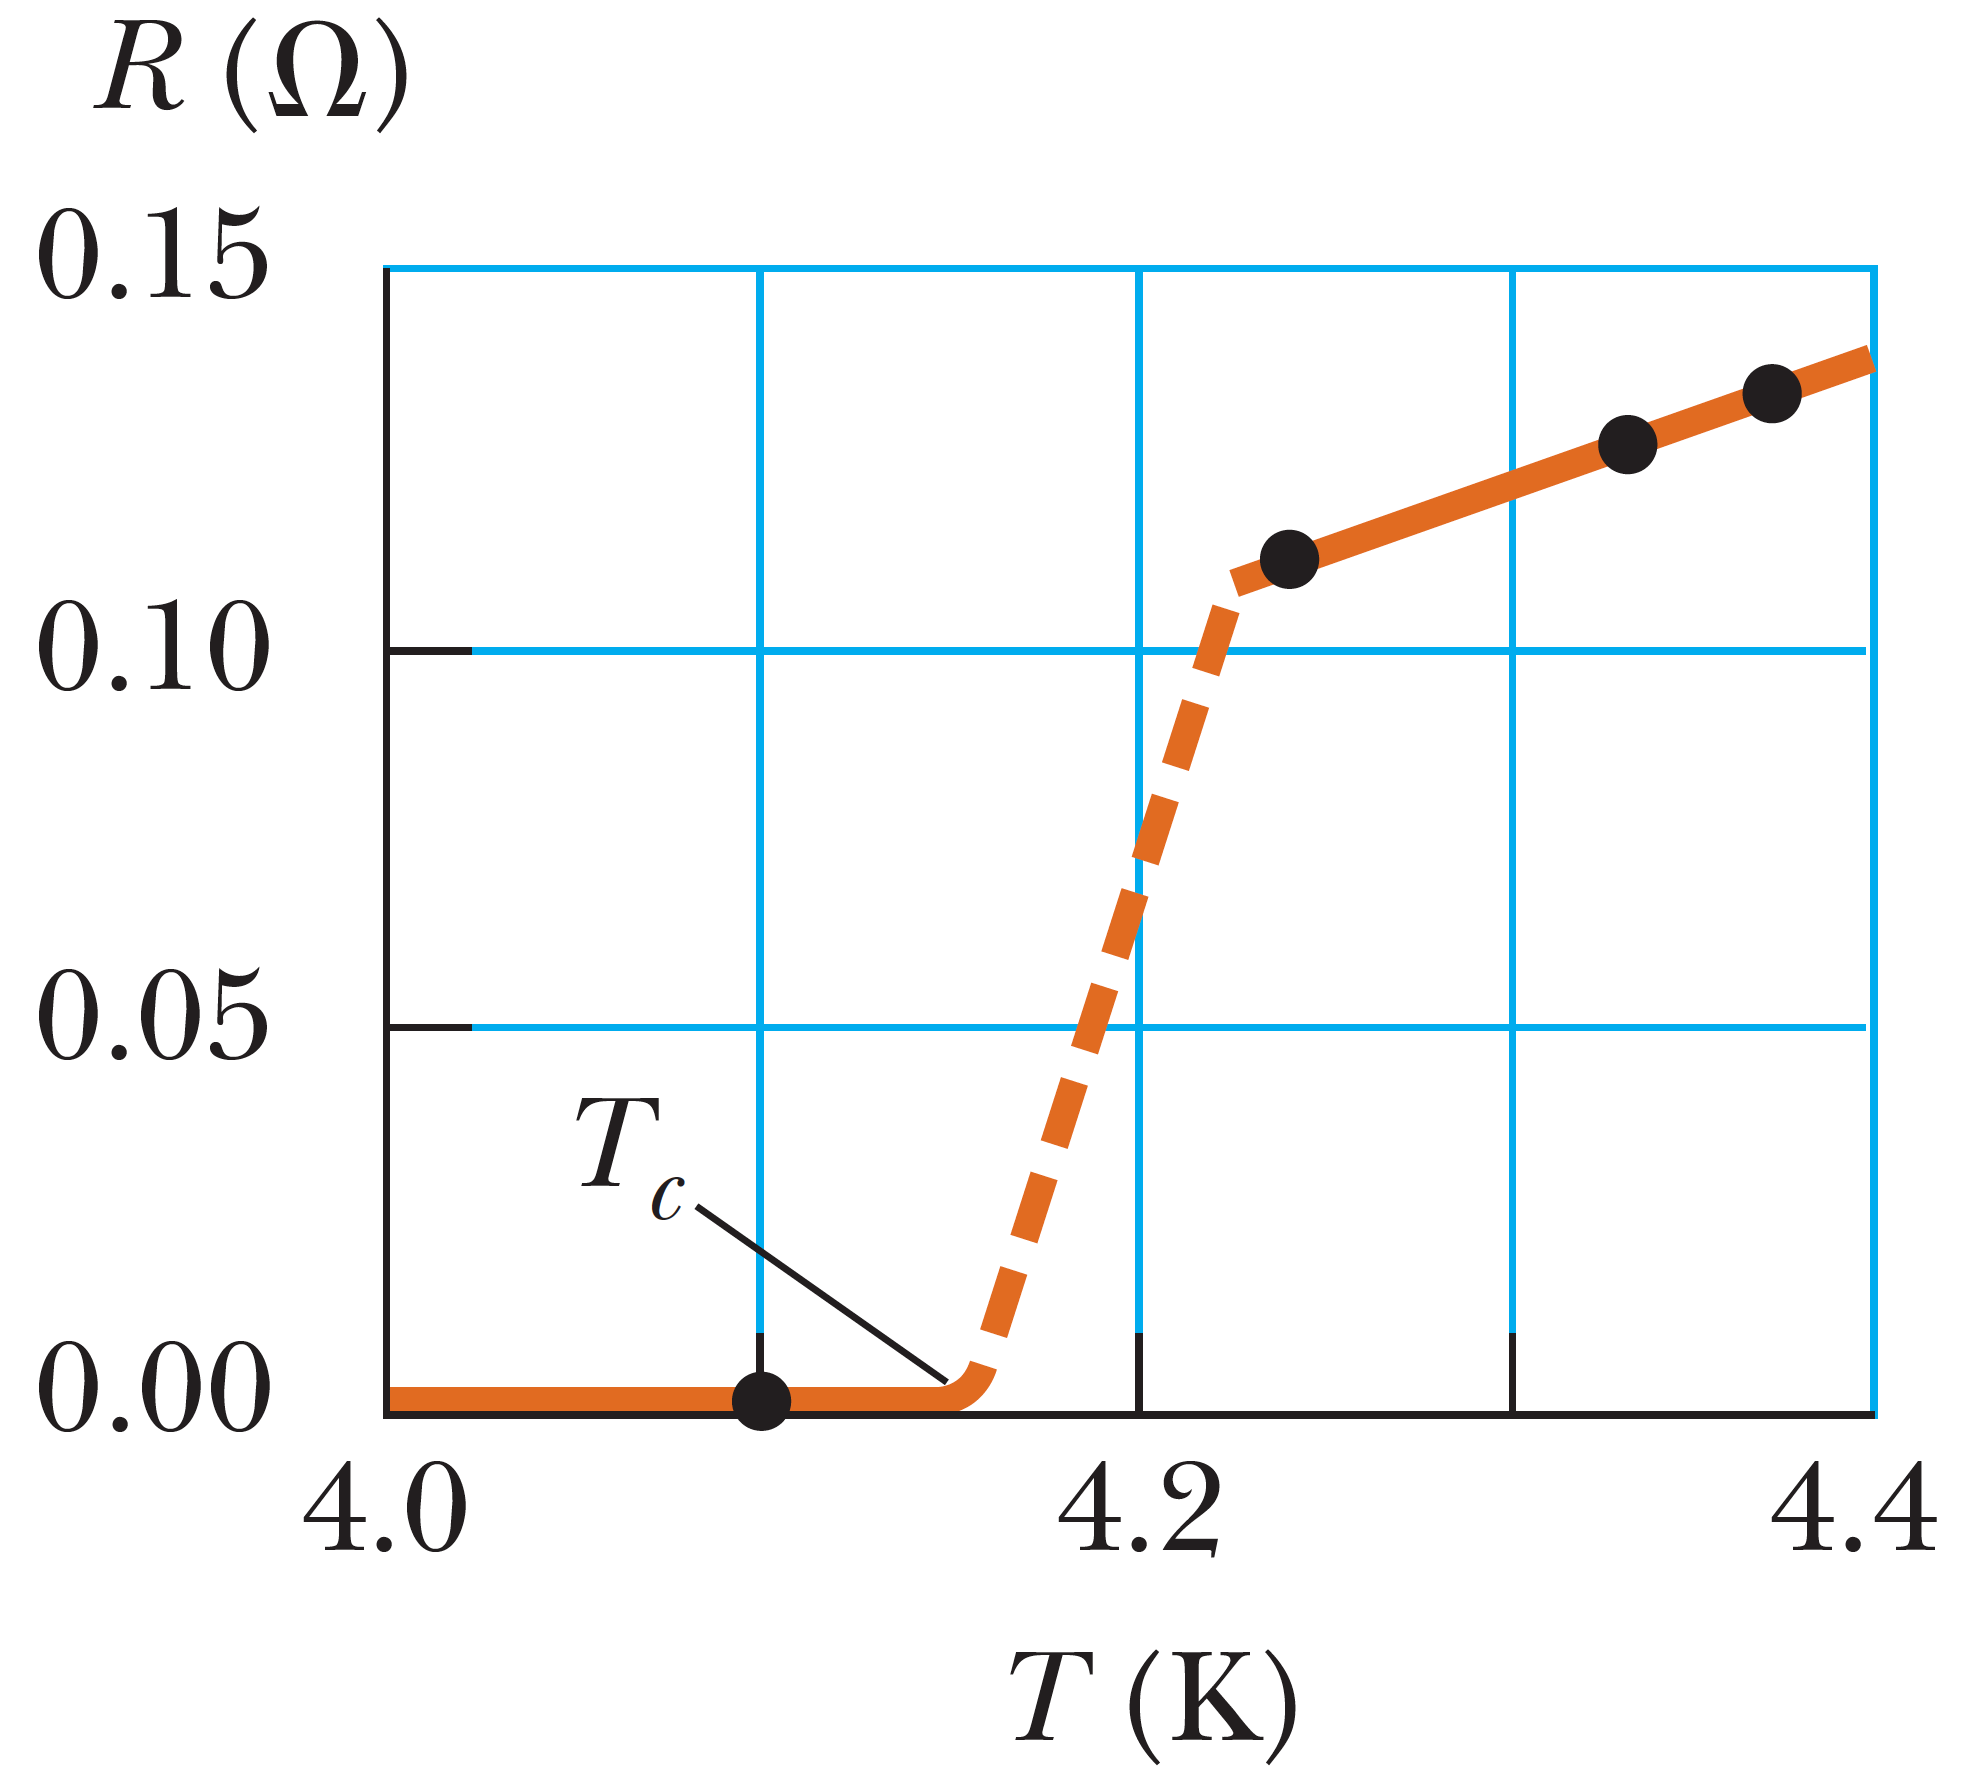
\includegraphics[width=0.35\textwidth]{4/figure_8}
    \caption{Resistencia en función de la temperatura para una muestra de mercurio (Hg).}
  \end{figure}

  \subsection{Potencia eléctrica}
    \PN En los circuitos eléctricos típicos, la energía se transfiere de una fuente, como una batería, a algún
    dispositivo, como sería una lámpara o un receptor de radio. Por ello conviene determinar una expresión que permita
    calcular la rapidez de transferencia de esta energía.

    \begin{figure}[H]
    \centering
      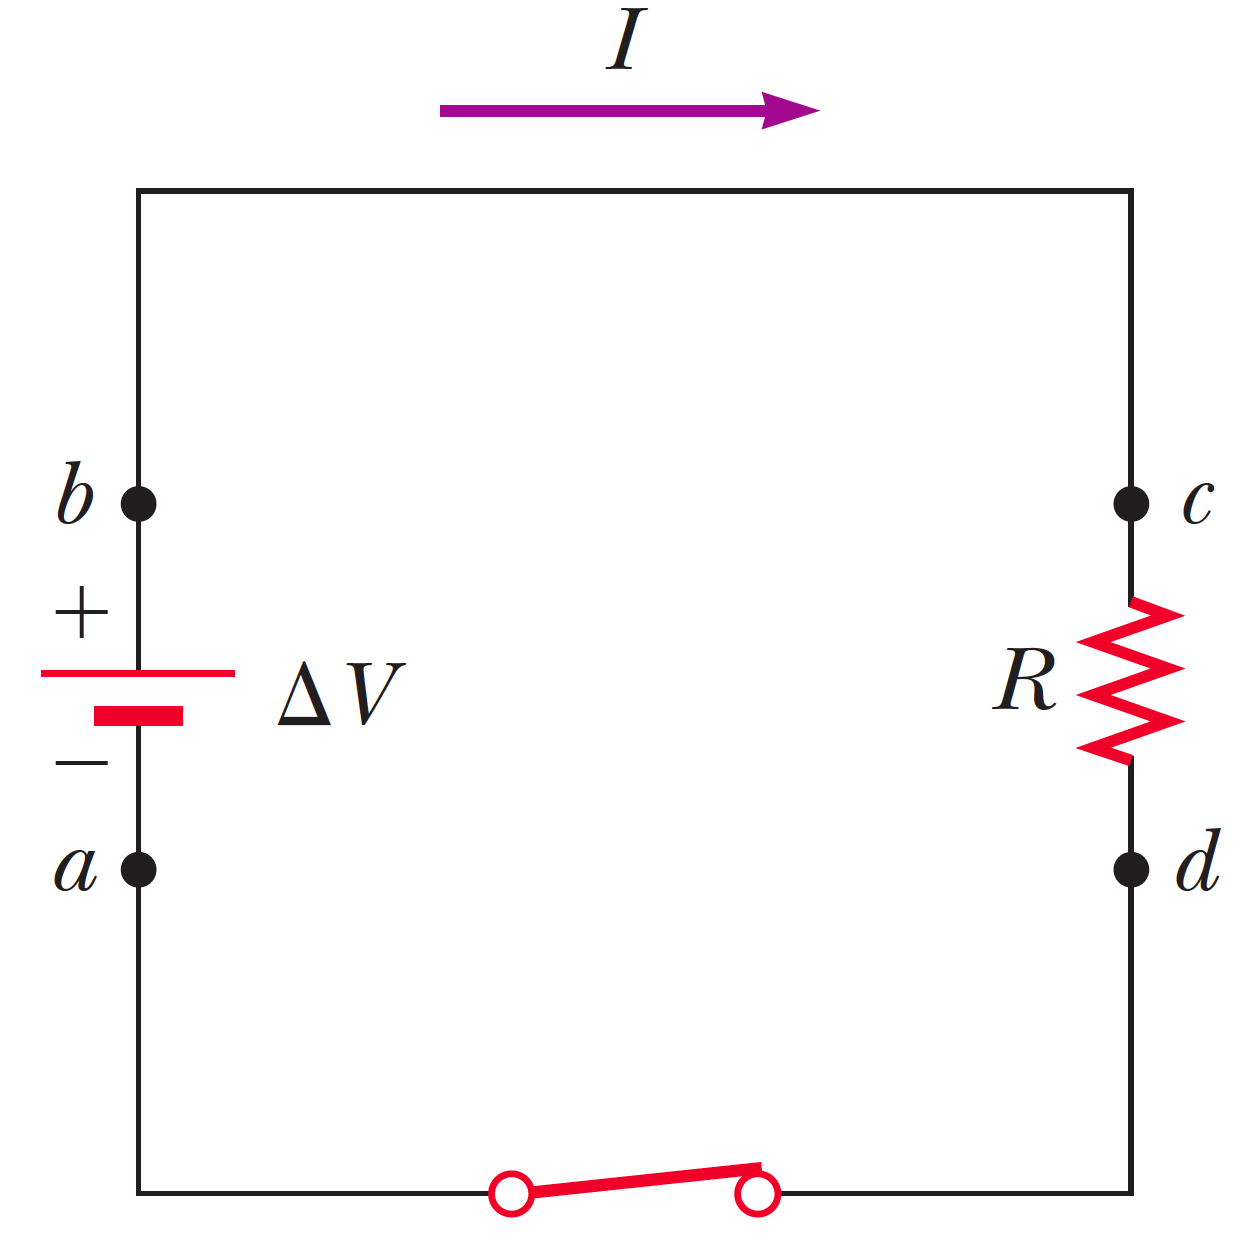
\includegraphics[width=0.25\textwidth]{4/figure_9}
      \caption{Circuito constituido por un resistor de resistencia $R$ y una batería con una diferencia de potencial
      $\Delta V$ entre sus terminales. La carga positiva fluye en dirección de las manecillas del reloj.}
    \end{figure}

    \PN Considere ahora la rapidez a la cual el sistema pierde energía potencial eléctrica conforme la carga $Q$ pasa a
    través del resistor:
    \begin{equation*}
      \frac{dU}{dt} = \frac{d}{dt} \ (Q \ \Delta V) = \frac{dQ}{dt} \ \Delta V = I \ \Delta V
    \end{equation*}

    \PN donde $I$ es la corriente en el circuito. El sistema recupera su energía potencial cuando la carga pasa a través
    de la batería, a expensas de la energía química de la misma. La rapidez a la cual el sistema pierde energía
    potencial conforme la carga pasa a través del resistor es igual a la rapidez a la cual el sistema adquiere energía
    interna en el resistor. Por lo tanto, la potencia $\mathcal{P}$ que representa la rapidez a la cual se entrega
    energía al resistor, es
    \begin{equation*}
      \mathcal{P} = I \ \Delta V
    \end{equation*}

    \PN Se deduce este resultado si considera una batería que entrega energía a un resistor. Para calcular la potencia
    entregada por una fuente de voltaje a cualquier dispositivo que tenga una corriente $I$ y esté sujeto a una
    diferencia de potencial $\Delta V$ entre sus terminales. Apartir de que un resistor $\Delta V = IR$, la potencia
    entregada al resistor tiene una expresión alterna
    \begin{equation*}
      \mathcal{P} = I^{2} R = \frac{(\Delta V)^{2}}{R}
    \end{equation*}

    \PN Cuando $I$ se expresa en amperes, $\Delta V$ en volts y $R$ en ohms, la unidad del SI para la potencia es el
    \textbf{watt}. El proceso mediante el que se pierde potencia en forma de energía interna en un conductor de
    resistencia $R$, a menudo se llama \textit{calentamiento joule}.

		\section{Circuitos de corriente directa}
  \subsection{Fuerza electromotriz}
    \PN Dado que en un circuito particular la diferencia de potencial en las terminales de la batería es constante, la
    corriente en el circuito es constante en magnitud y dirección y recibe el nombre de corriente directa. A la batería se
    le conoce como fuente de fuerza electromotriz, o más comúnmente, \textit{fuente de fem}. (Lo que se conoce como
    \textbf{fuerza electromotriz} es un desafortunado equívoco histórico, pues describe no una fuerza, sino una diferencia
    de potencial en volts.) La fem $\varepsilon$ de una batería es el voltaje máximo posible que ésta puede suministrar
    entre sus terminales.

    \begin{figure}[H]
    \centering
      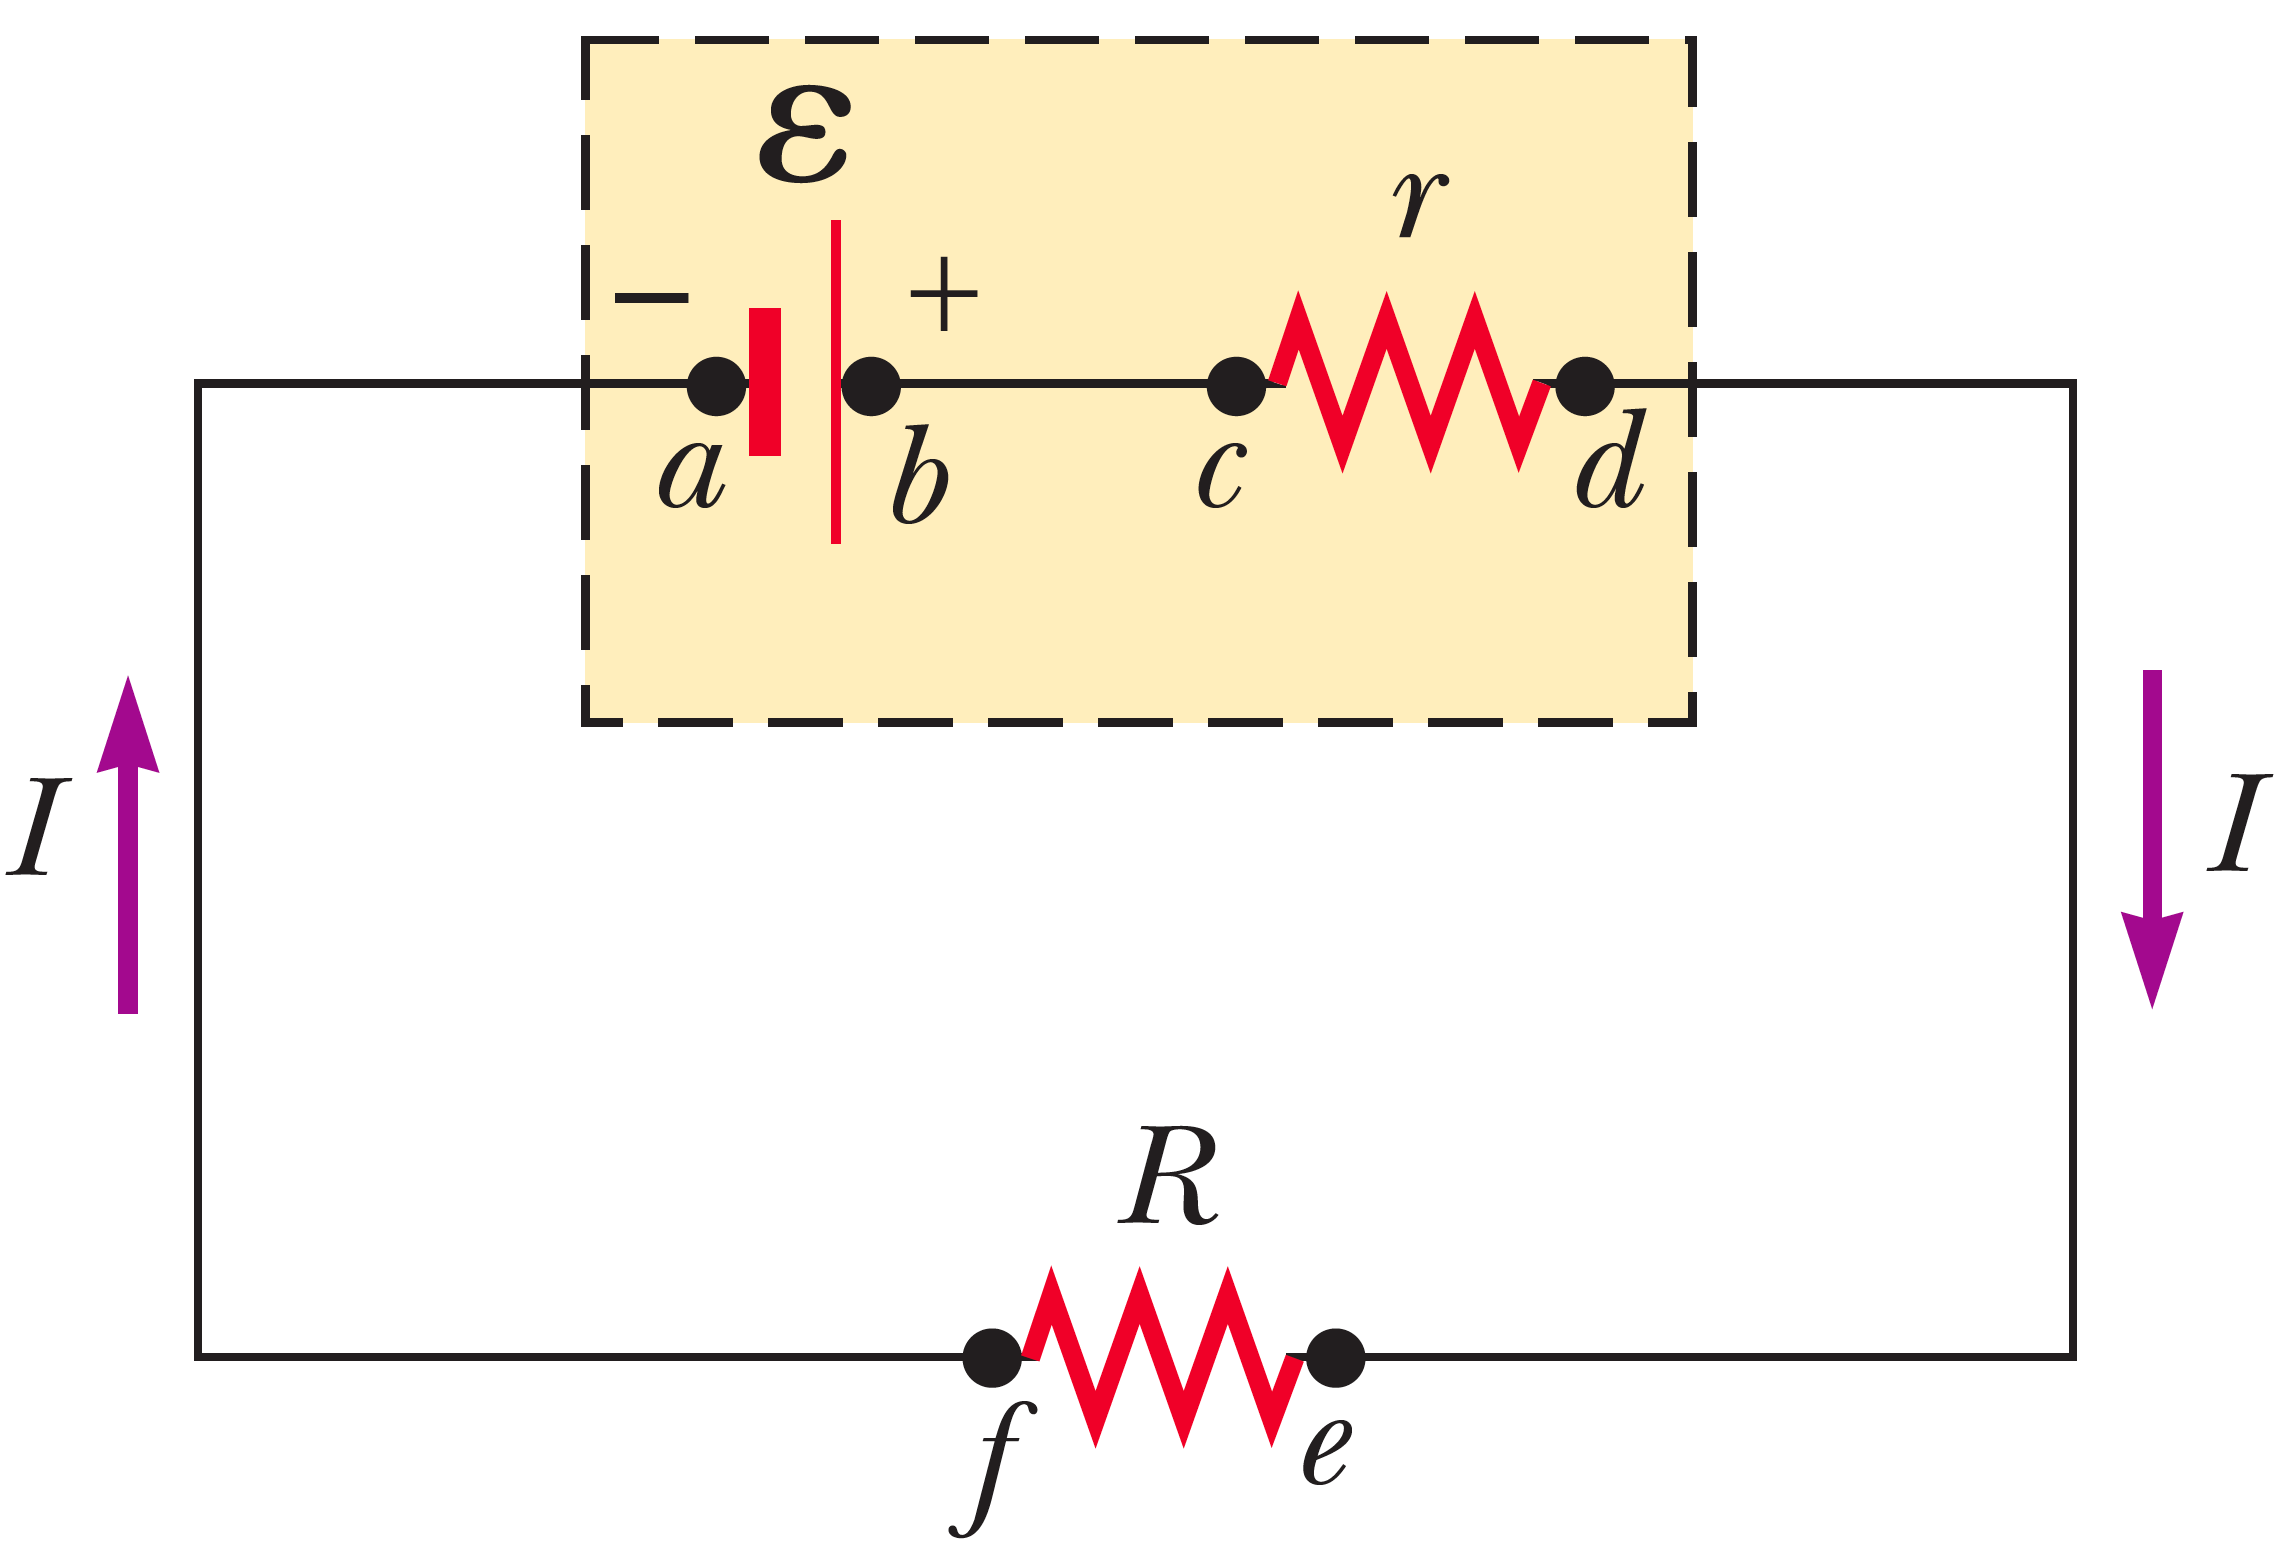
\includegraphics[width=0.35\textwidth]{4/figure_10}
      \caption{Diagrama de un circuito de una fuente de fem $\varepsilon$ (en este caso, una batería), de resistencia
      interna $r$, conectada a un resistor externo, de resistencia $R$.}
    \end{figure}

    \PN La terminal positiva de la batería se encuentra a un potencial más alto que la negativa. Puesto que una batería
    está hecha de materia, existe una resistencia al flujo de las cargas dentro de la misma. Esta resistencia recibe el
    nombre de \textbf{resistencia interna} $r$. En el caso de una batería ideal con una resistencia interna igual a cero,
    la diferencia de potencial a través de la batería (conocida como voltaje entre las terminales) es igual a su fem. El
    el voltaje entre las terminales de la batería $\Delta V = V_{d} - V_{a}$ es:
    \begin{equation*}
      \Delta V = \varepsilon - I r
    \end{equation*}

    \PN Notar que $\varepsilon$ es equivalente al \textbf{voltaje en circuito abierto}, es decir, el voltaje entre las
    terminales cuando la corriente es igual a cero. La diferencia de potencial real entre las terminales de la batería
    depende de la corriente en la misma.

    \VS
    \PN El voltaje entre las terminales $\Delta V$ debe ser igual a la diferencia de potencial de un extremo a otro de la
    resistencia externa $R$, conocida como \textbf{resistencia de carga}. El resistor representa una carga en la batería
    porque ésta debe suministrar energía para que el aparato que contiene la resistencia funcione. La diferencia de
    potencial de un extremo a otro de la resistencia de carga es $\Delta V = IR$.
    \begin{equation*}
      \varepsilon = IR + Ir
    \end{equation*}

    \PN Al resolver en función de la corriente
    \begin{equation*}
      I = \frac{\varepsilon}{R + r}
    \end{equation*}

    \PN Esta ecuación muestra que la corriente en este circuito simple depende tanto de la resistencia de carga $R$
    externa a la batería como de la resistencia interna $r$. Si $R$ es mucho mayor que $r$, como es el caso de muchos
    circuitos útiles en la vida cotidiana, ignore $r$, es decir:
    \begin{equation*}
      \varepsilon = IR
    \end{equation*}

  \subsection{Resistores en serie y en paralelo}
    \subsubsection{Resistores en serie}

      \begin{figure}[H]
      \centering
        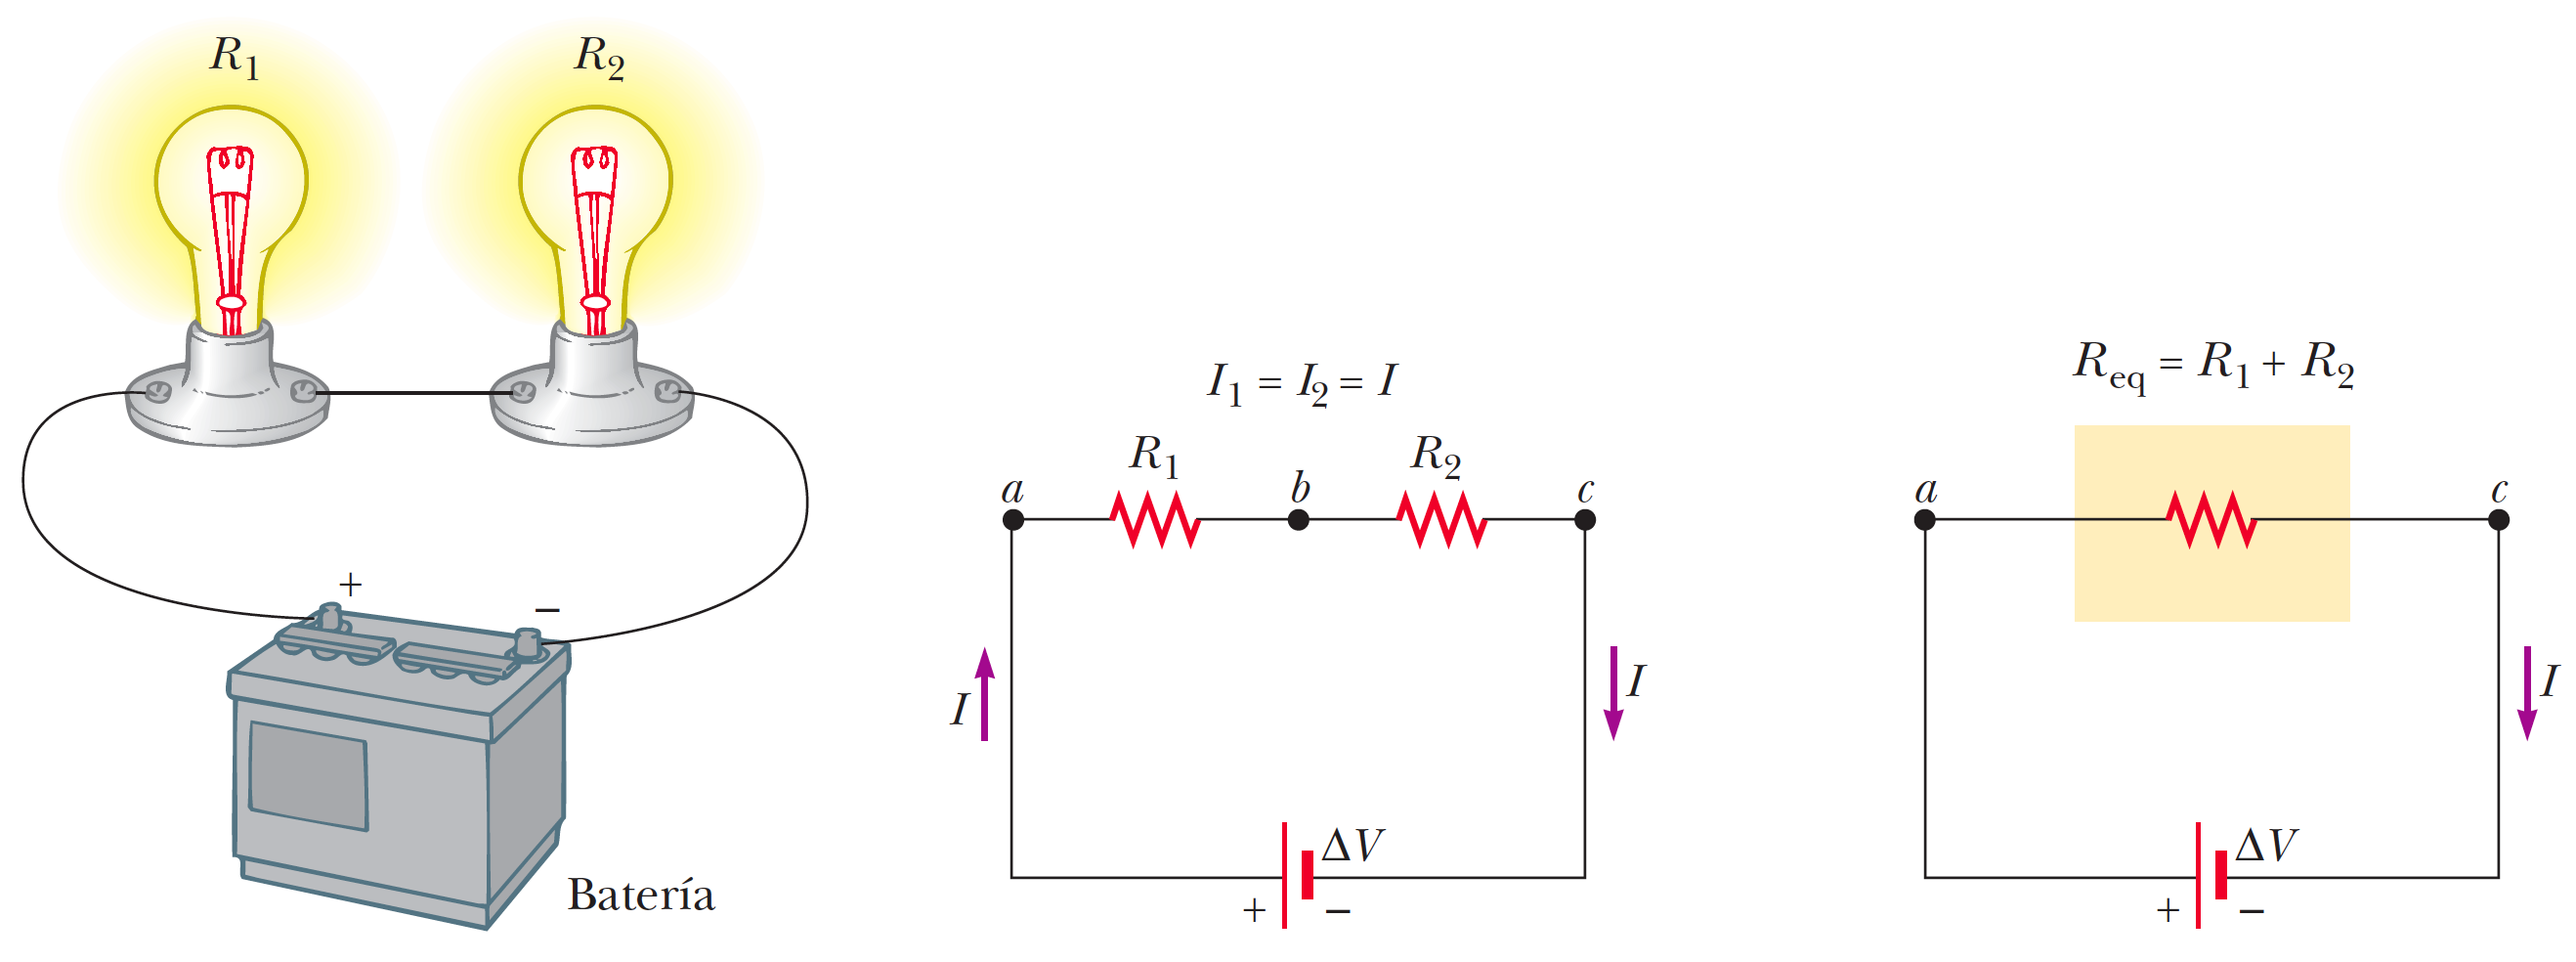
\includegraphics[width=0.7\textwidth]{4/figure_11}
        \caption{Diagrama de un circuito de una fuente de fem $\varepsilon$ (en este caso, una batería), de resistencia
        interna $r$, conectada a un resistor externo, de resistencia $R$.}
      \end{figure}

      \PN Cuando dos o más resistores están interconectados como los de la figura anterior, se dice que están en una
      \textbf{combinación en serie}. En una conexión en serie, si una cantidad de carga $Q$ sale de un resistor $R_{1}$,
      deberá también entrar en el segundo resistor $R_{2}$. Por lo tanto, en un intervalo determinado de tiempo, la
      misma cantidad de carga pasa a través de ambos resistores.
      \begin{equation*}
        I = I_{1} = I_{2}
      \end{equation*}

      \PN donde $I$ es la corriente de la batería, $I_{1}$ es la corriente en el resistor $R_{1}$ e $I_{2}$ es la
      corriente en el resistor $R_{2}$.

      \VS
      \PN La diferencia de potencial que se aplica a una combinación en serie de resistores se dividirá entre éstos. En
      la figura, ya que la caída de voltaje de $a$ a $b$ es igual a $I_{1}R_{1}$ y la caída de voltaje de $b$ a $c$ es
      \begin{equation*}
        \Delta V = I_{1}R_{1} + I_{2}R_{2}
      \end{equation*}

      \PN La diferencia de potencial entre las terminales de la batería también está aplicada a la resistencia
      equivalente $R_{eq}$:
      \begin{equation*}
        \Delta V = I R_{eq}
      \end{equation*}

      \PN donde la resistencia equivalente tiene el mismo efecto en el circuito que en la combinación en serie porque
      resulta de la misma corriente $I$ en la batería. Al combinar estas ecuaciones para $\Delta V$ se sustituyen los
      dos resistores en serie por una sola resistencia equivalente, cuyo valor es la \textit{suma} de las resistencias
      equivalentes:
      \begin{equation*}
        \Delta V = I R_{eq} = I_{1}R_{1} + I_{2}R_{2} \rightarrow R_{eq} = R_{1} + R_{2}
      \end{equation*}

      \PN La resistencia equivalente de tres o más resistores conectados en serie es
      \begin{equation*}
        R_{eq} = R_{1} + R_{2} + R_{3} + \dotsc
      \end{equation*}

      \PN Esta correspondencia indica que \textbf{la resistencia equivalente de una combinación en serie de resistores
      es la suma numérica de las resistencias individuales y siempre es mayor que cualquier resistencia individual}.

    \subsubsection{Resistores en paralelo}

      \begin{figure}[H]
      \centering
        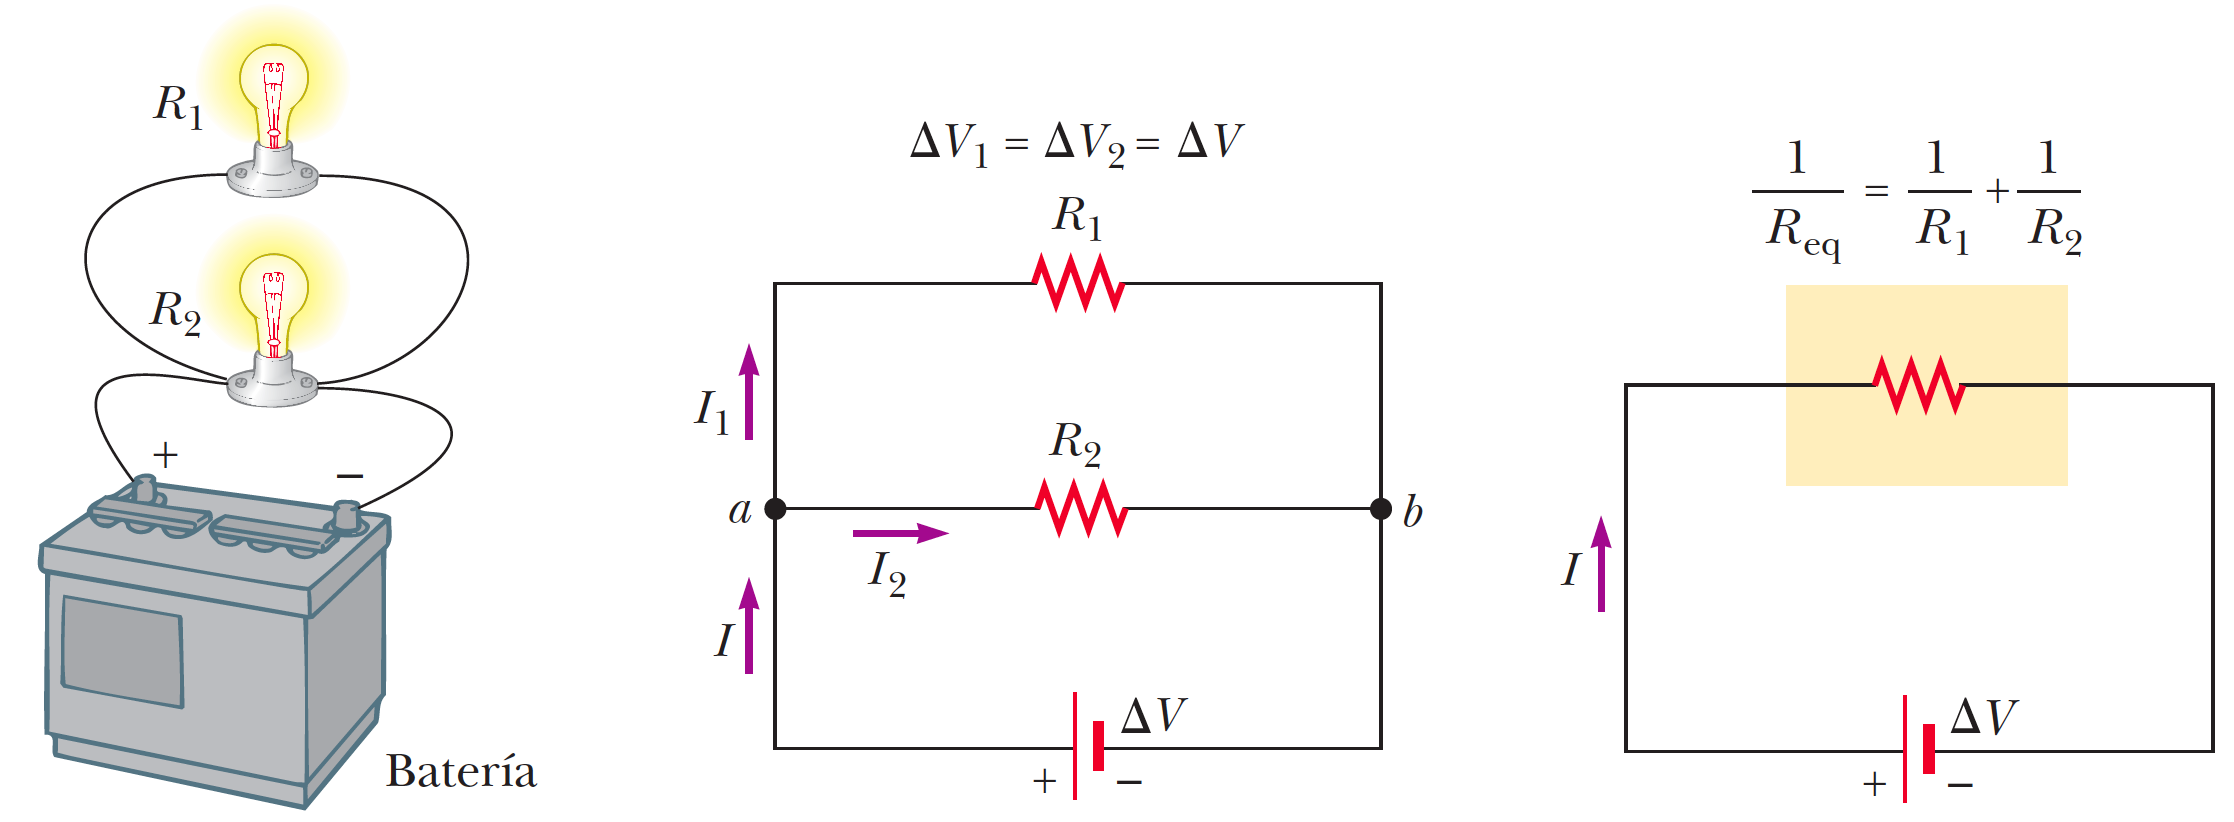
\includegraphics[width=0.7\textwidth]{4/figure_12}
        \caption{Diagrama de un circuito de una fuente de fem $\varepsilon$ (en este caso, una batería), de resistencia
        interna $r$, conectada a un resistor externo, de resistencia $R$.}
      \end{figure}

      \PN En una \textbf{combinación en paralelo}, las diferencias de potencial a través de los resistores son las
      mismas:
      \begin{equation*}
        \Delta V = \Delta V_{1} = \Delta V_{2}
      \end{equation*}

      \PN donde $\Delta V$es el voltaje entre las terminales de la batería.

      \VS
      \PN Cuando las cargas llegan al punto $a$ en la figura b), se dividen en dos; una parte pasa a través de $R_{1}$ y
      el resto a través de $R_{2}$. Una unión es cualquier punto en un circuito donde una corriente puede dividirse.
      Esta división resulta en menos corriente en cada resistor de la que sale de la batería. Debido a que la carga
      eléctrica se conserva, la corriente $I$ que entra al punto a debe ser igual a la corriente total que sale del
      mismo:
      \begin{equation*}
        I = I_{1} + I_{2}
      \end{equation*}

      \PN donde $I_{1}$ es la corriente en $R_{1}$ e $I_{2}$ es la corriente en $R_{2}$.

      \VS
      \PN La corriente en la resistencia equivalente $R_{eq}$ es
      \begin{equation*}
        I = \frac{\Delta V}{R_{eq}}
      \end{equation*}

      \PN donde la resistencia equivalente tiene el mismo efecto en el circuito que las dos resistencias en paralelo,
      por lo que la resistencia equivalente de dos resistores en paralelo se conoce por
      \begin{equation*}
        I = \frac{\Delta V}{R_{eq}} = \frac{\Delta V_{1}}{R_{1}} + \frac{\Delta V_{2}}{R_{2}} \rightarrow
        \frac{1}{R_{eq}} = \frac{1}{R_{1}} + \frac{1}{R_{2}}
      \end{equation*}

      \PN Una extensión de esta explicación a tres o más resistores en paralelo da:
      \begin{equation*}
        \frac{1}{R_{eq}} = \frac{1}{R_{1}} + \frac{1}{R_{2}} + \frac{1}{R_{3}} + \dotsc
      \end{equation*}

      \PN De esta expresión se ve que \textbf{el inverso de la resistencia equivalente de dos o más resistores
      conectados en una combinación en paralelo es igual a la suma de los inversos de las resistencias individuales.
      Además, la resistencia equivalente siempre es menor que la resistencia más pequeña en el grupo}.

    \subsection{Leyes de Kirchhoff}
      \PN Es posible simplificar y explicar combinaciones de resistores aplicando la expresión $\Delta V = IR$ y las
      reglas para las combinaciones en serie y en paralelo de los resistores. Muy a menudo, sin embargo, no es posible
      simplificar un circuito en una sola espira. El procedimiento para explicar circuitos más complejos se hace
      posible si se utilizan dos principios conocidos como leyes de Kirchhoff:

      \begin{itemize}
        \item \textbf{Ley de la unión:} En cualquier unión, la suma de las corrientes debe ser igual a cero:
        \begin{equation*}
          \sum_{union} I = 0
        \end{equation*}

        \item \textbf{Ley de la espira:} La suma de las diferencias de potencial a través de todos los elementos
        alrededor de cualquier espira de un circuito cerrado debe ser igual a cero:
        \begin{equation*}
          \sum_{espira} \ \Delta V = 0
        \end{equation*}
      \end{itemize}

      \PN La primera ley de Kirchhoff es un enunciado de la conservación de la carga eléctrica. La segunda ley de
      Kirchhoff es una consecuencia de la ley de conservación de energía.

      \VS
      \PN Las siguientes son reglas para determinar las diferencias de potencial a través de un resistor y de una
      batería, utilizando la segunda ley y bajo la supocición de que la batería no tiene resistencia interna. Cada
      elemento del circuito se recorre de $a$ hasta $b$, de izquierda a derecha.
      \begin{multicols}{2}
        \begin{itemize}
          \item las cargas se mueven del extremo de potencial alto de un resistor hacia el extremo de potencial bajo; si
          un resistor se atraviesa en la dirección de la corriente, la diferencia de potencial $\Delta V$ a través del
          resistor es $-IR$ (figura a)).
          \item si un resistor se recorre en la dirección opuesta a la corriente, la diferencia de potencial $\Delta V$ a
          través del resistor es $+IRR$ (figura b)).
          \item Si una fuente de fem (suponiendo que tenga una resistencia interna igual a cero) es recorrida en la
          dirección de la fem (de negativo a positivo), la diferencia de potencial $\Delta V$ es $+\varepsilon$
          (figura c)).
        	\item si una fuente de fem (suponiendo que tenga una resistencia interna igual a cero) es recorrida en la
          dirección opuesta a la fem (de positivo a negativo), la diferencia de potencial $\Delta V$ es $-\varepsilon$
          (figura d)).
        \end{itemize}

        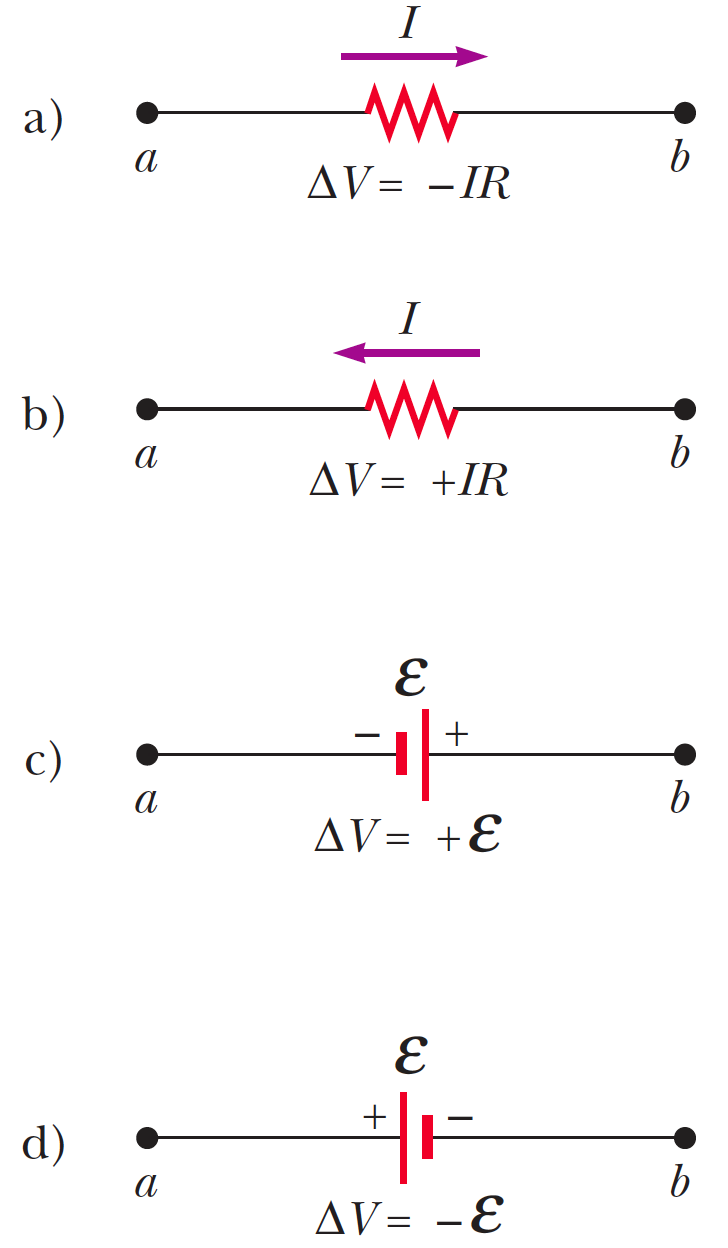
\includegraphics[width=0.4\textwidth]{4/figure_13}\par
      \end{multicols}

      \PN En general, para resolver un problema de circuito en particular, el número de ecuaciones independientes que se
      necesitan para obtener las dos leyes es igual al número de corrientes desconocidas.

\end{document}
